\section{Downstream metrics}

\subsection{Nuclei segmentation}
\subsubsection{Challenge}
\begin{figure}[H]
    \centering
    \setkeys{Gin}{width=\linewidth}
    \centering
        \begin{tabularx}{\textwidth}{YYYY}
            \textbf{Too few cells} &
            \textbf{Overexposure} &
            \textbf{Light gradient} &
            \textbf{Normal lightning} \\
            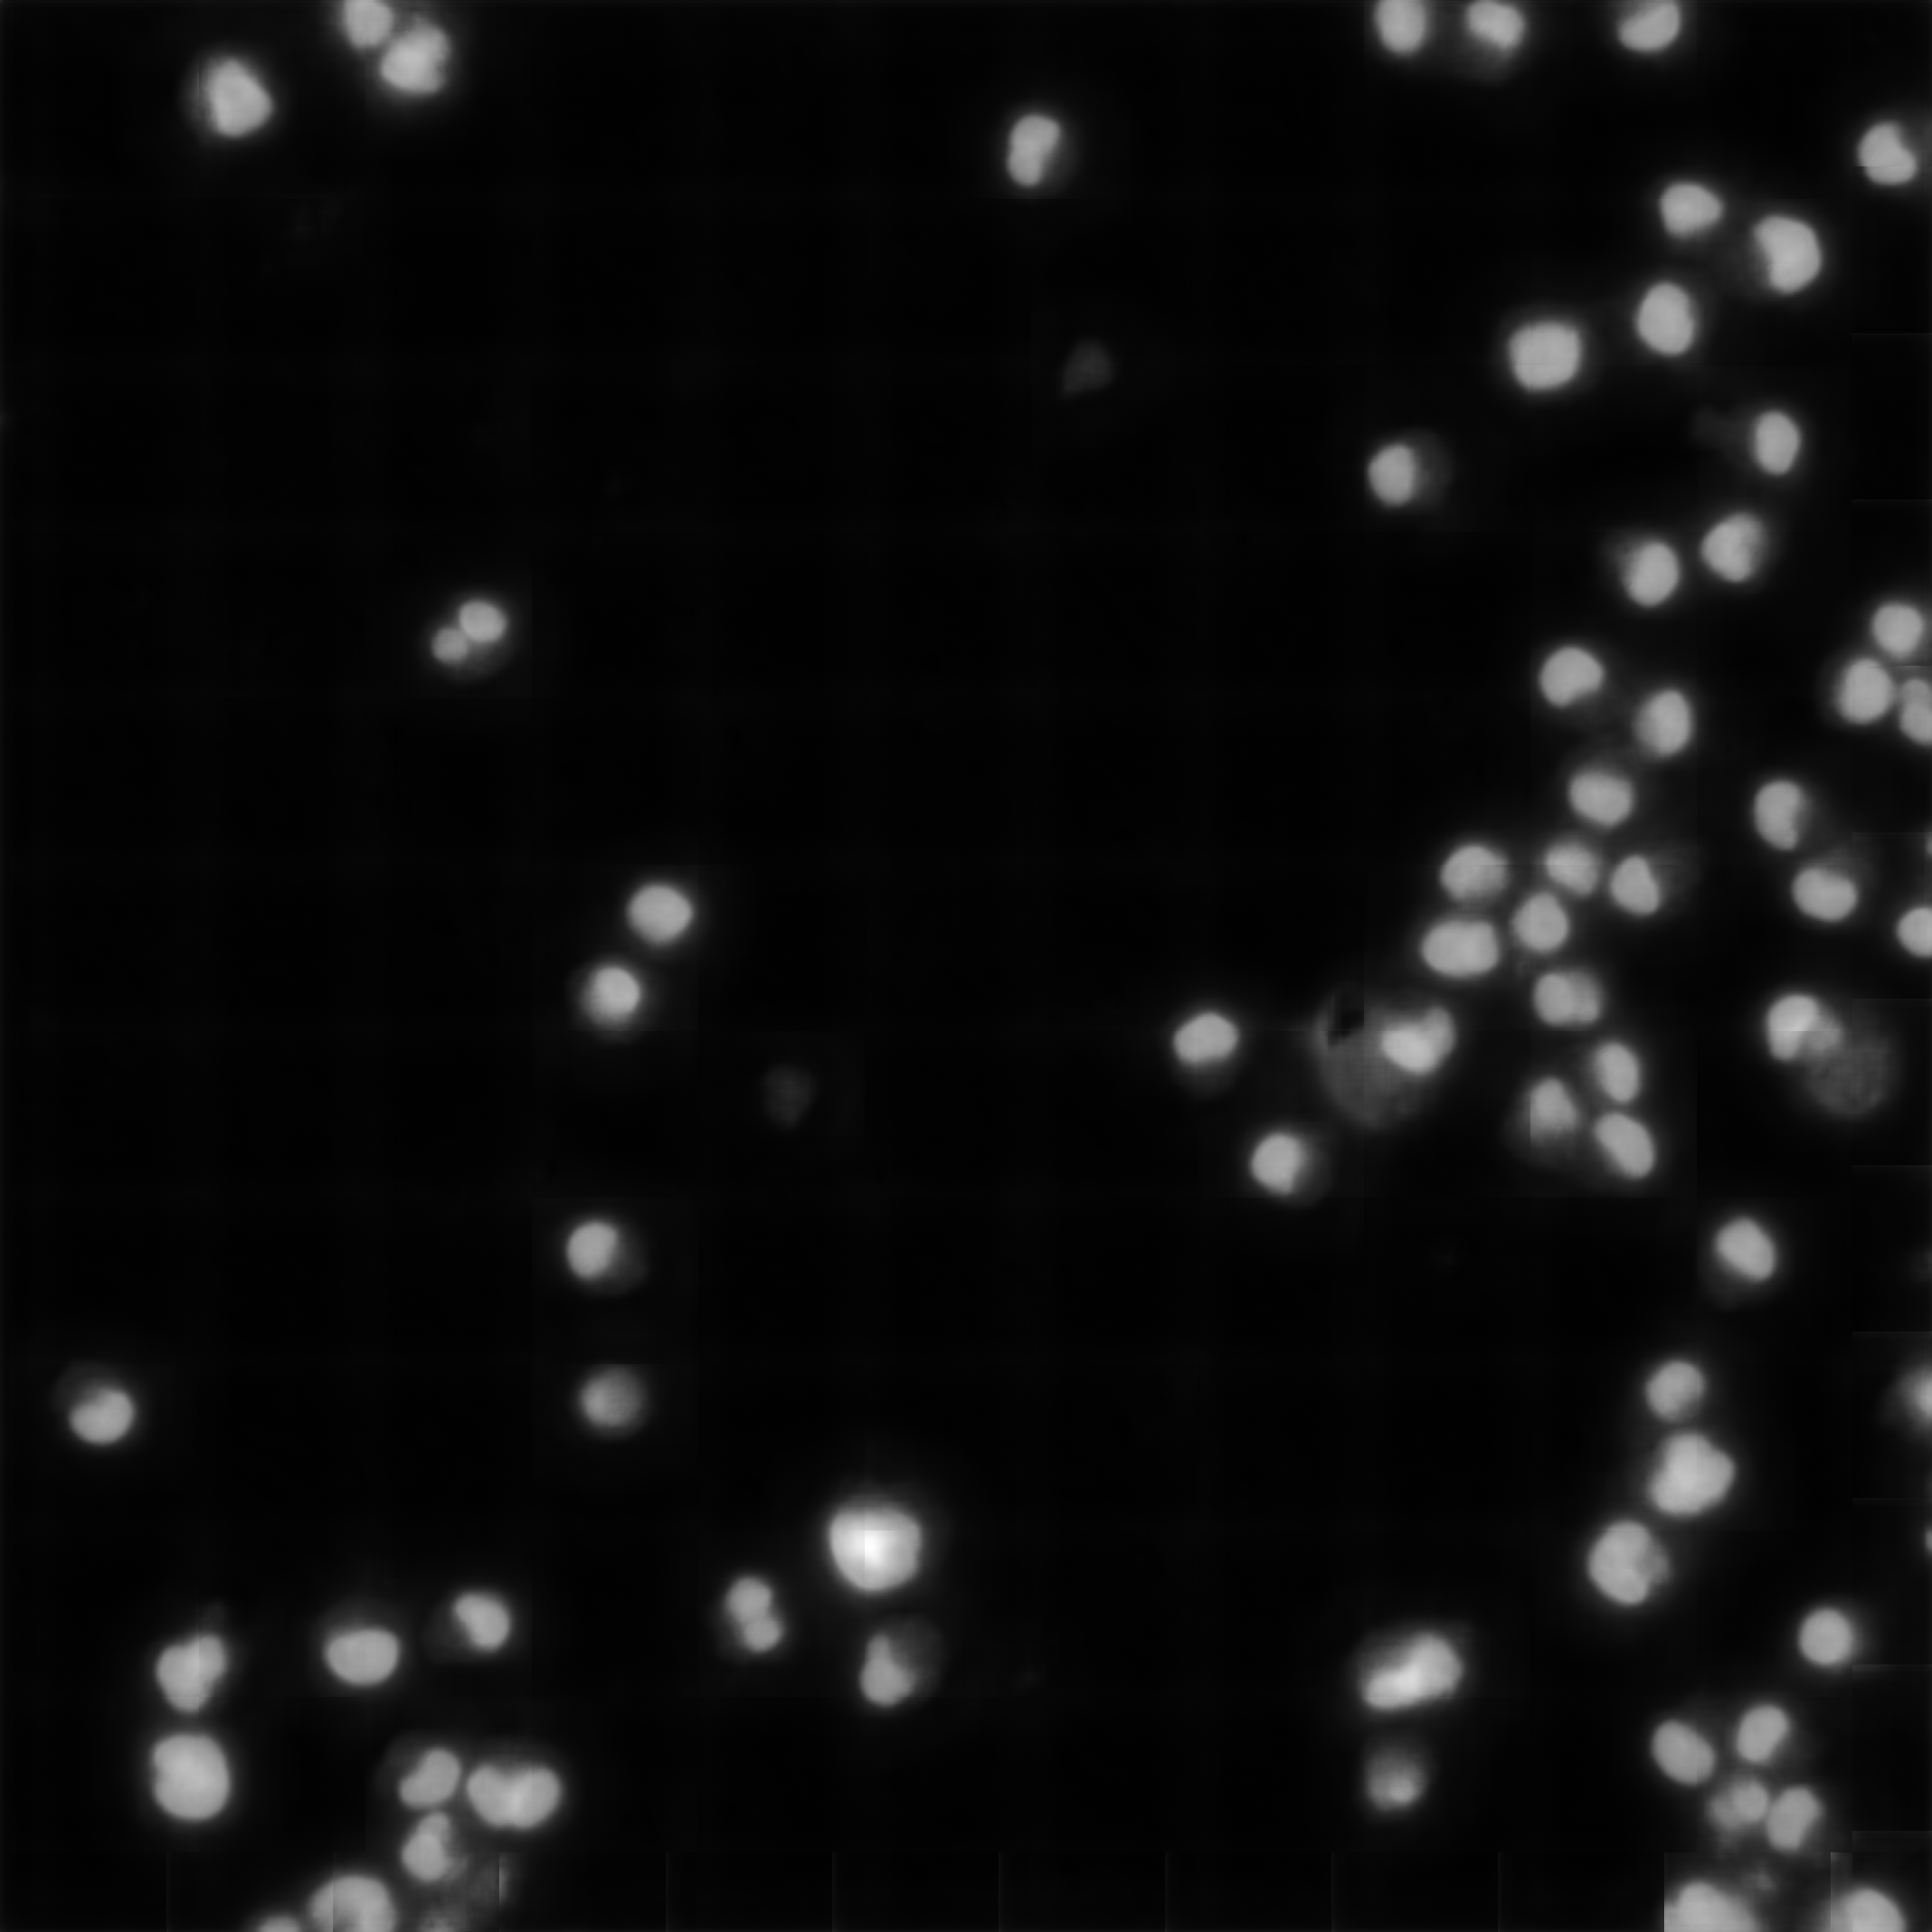
\includegraphics{bilder/lightning-conditions/lightning-1.png} & 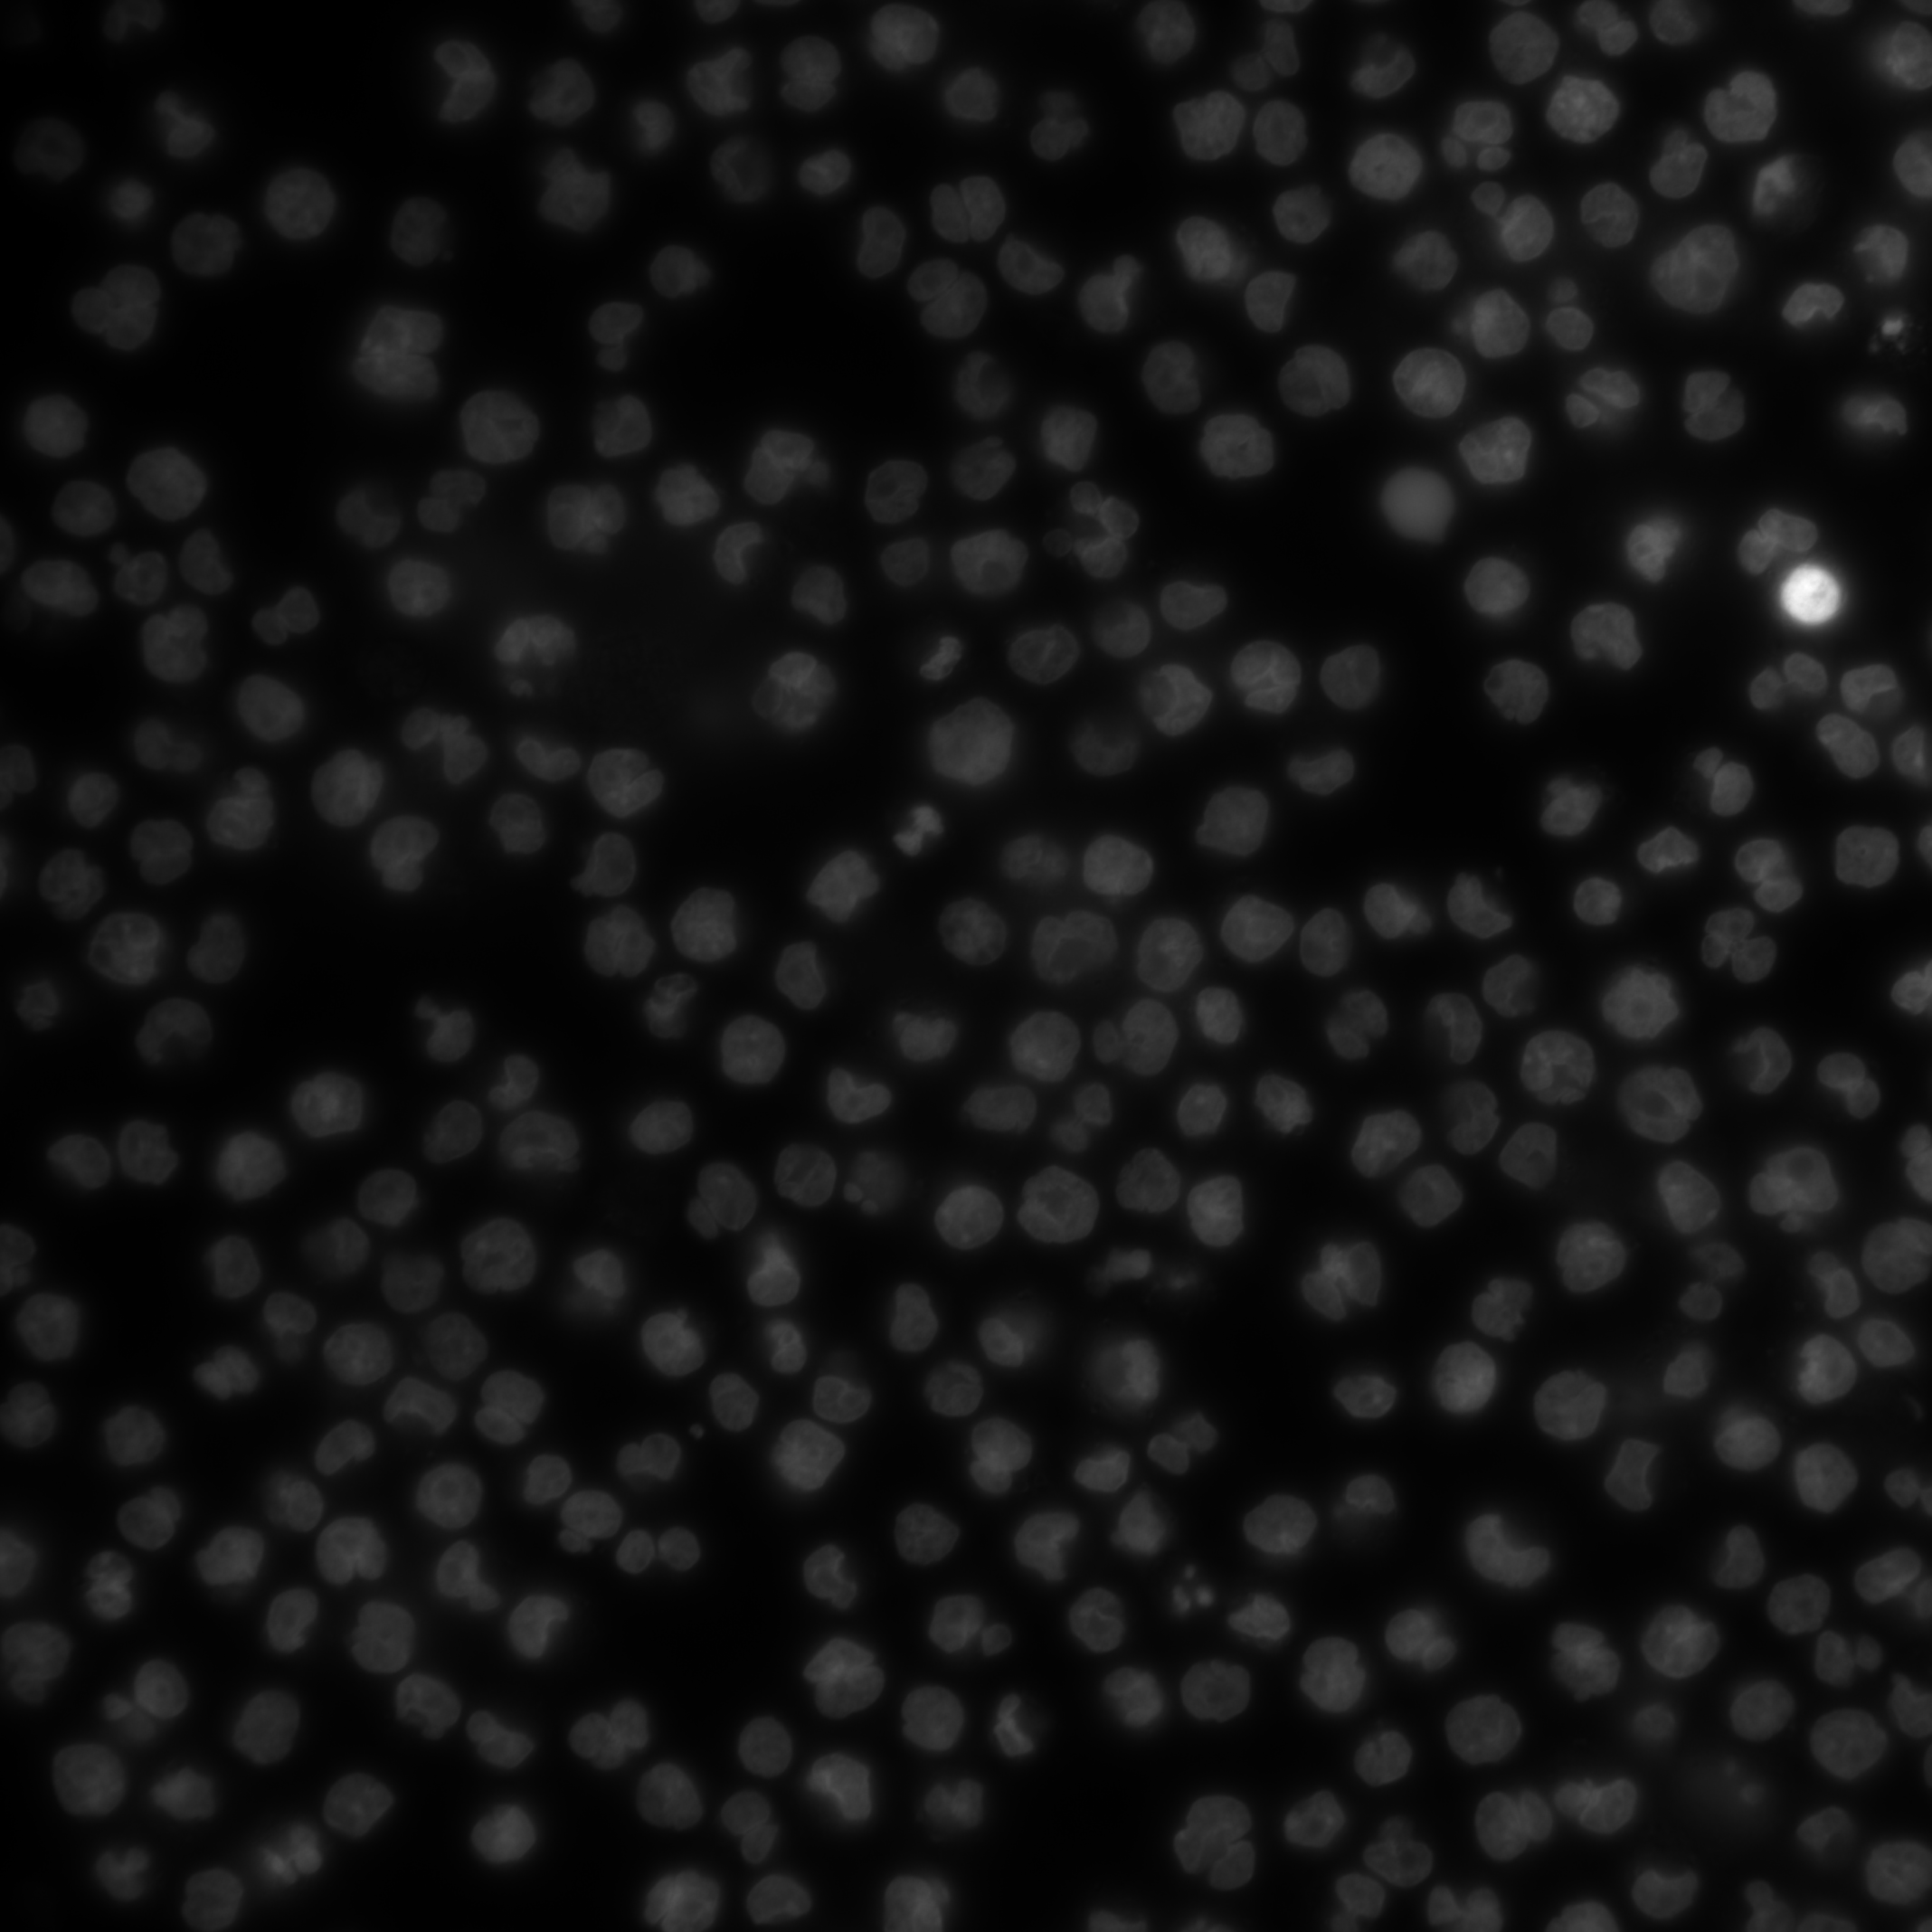
\includegraphics{bilder/lightning-conditions/lightning-2.png} &
            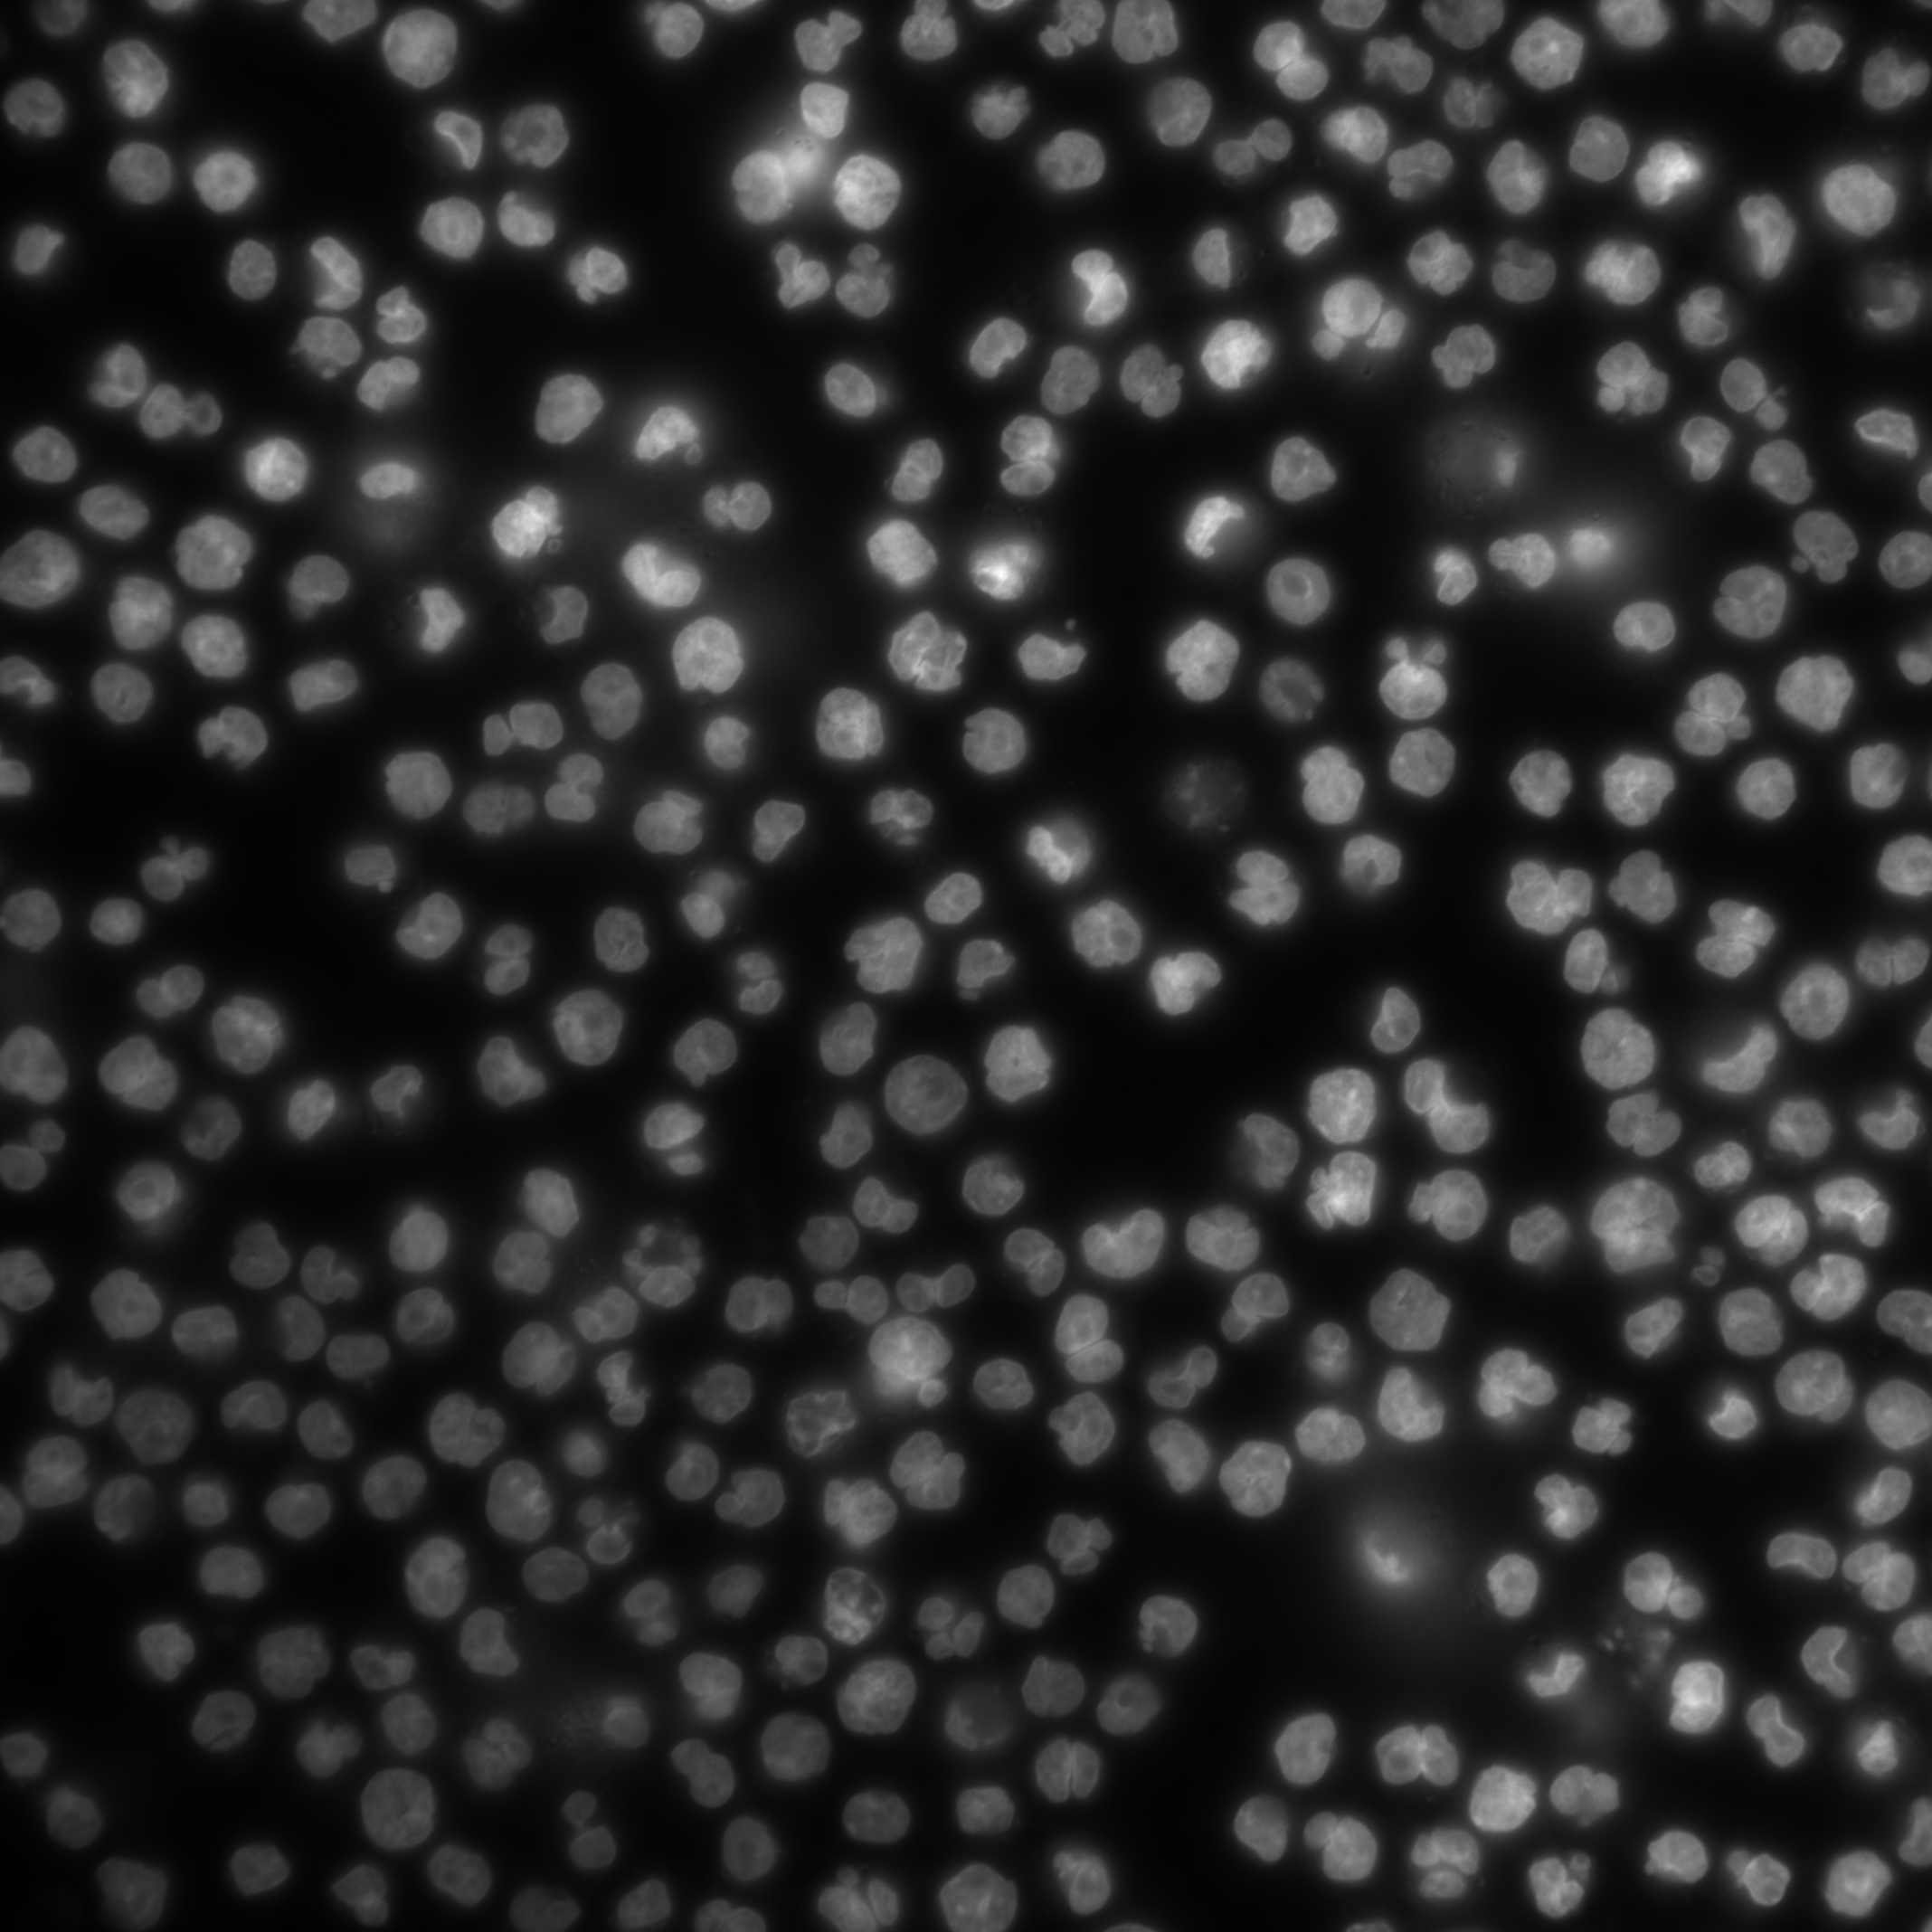
\includegraphics{bilder/lightning-conditions/lightning-3.png} & 
            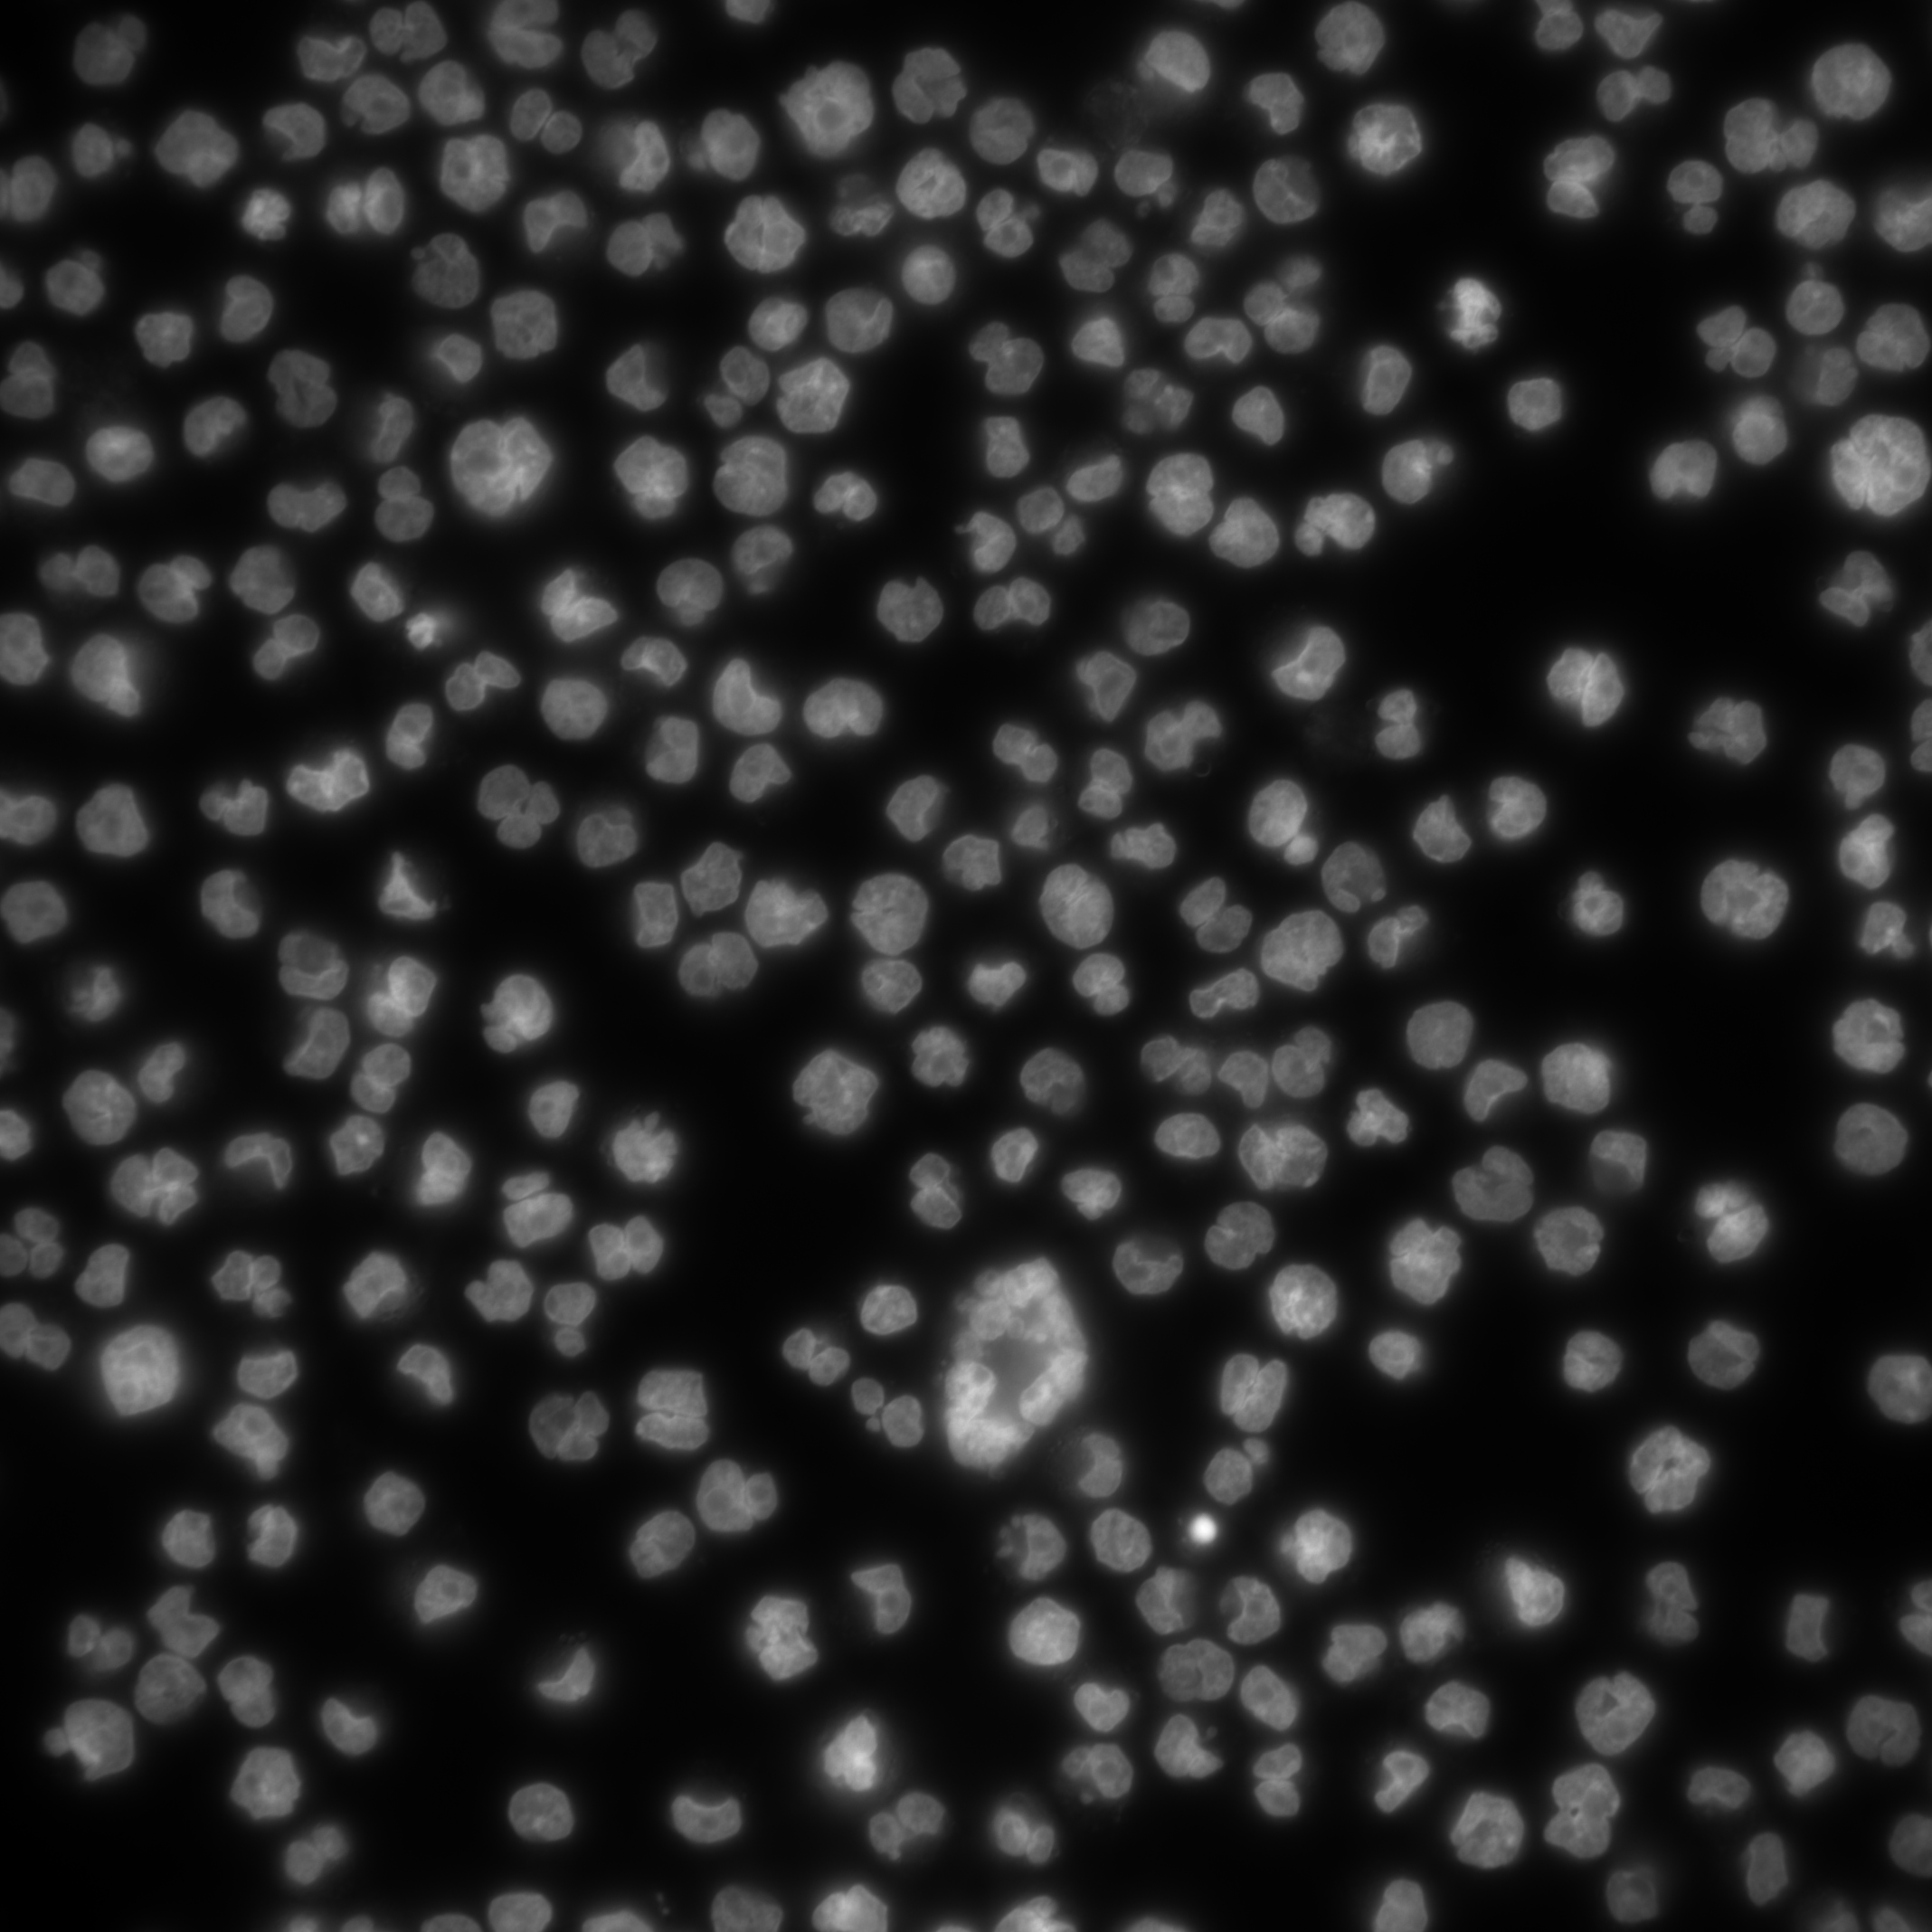
\includegraphics{bilder/lightning-conditions/lightning-4.png}
        \end{tabularx}
    \caption{Different lightning conditions}
    \label{fig:lightning_conditions}
\end{figure}

\begin{figure}[H]
    \centering
    \setkeys{Gin}{width=\linewidth}
    \centering
        \begin{tabularx}{\textwidth}{YY}
            \textbf{Original fluorescence} &
            \textbf{Segmentation} \\
            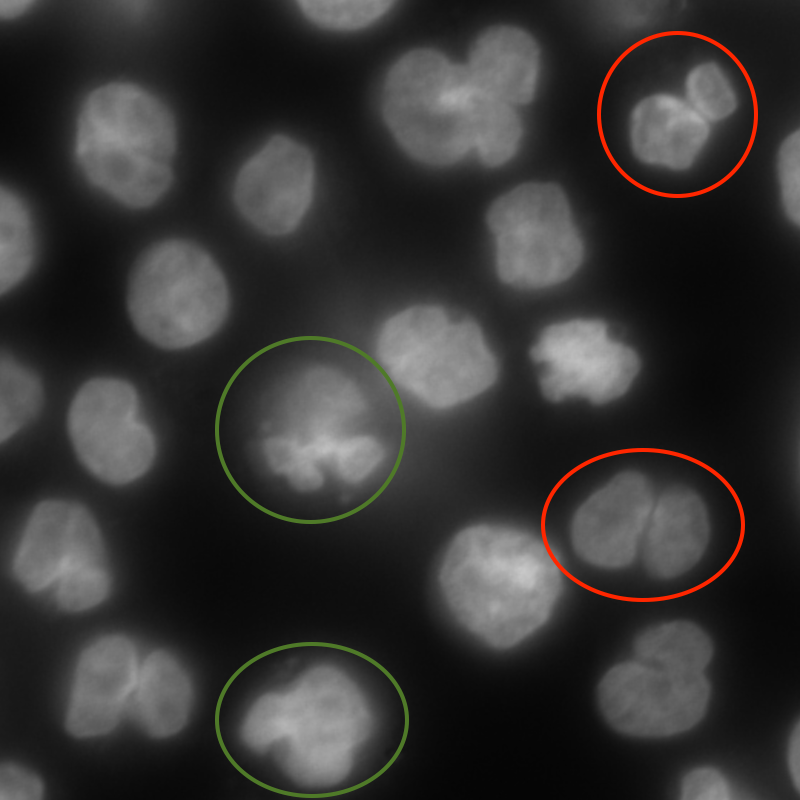
\includegraphics{bilder/close-located-cells/original.png} & 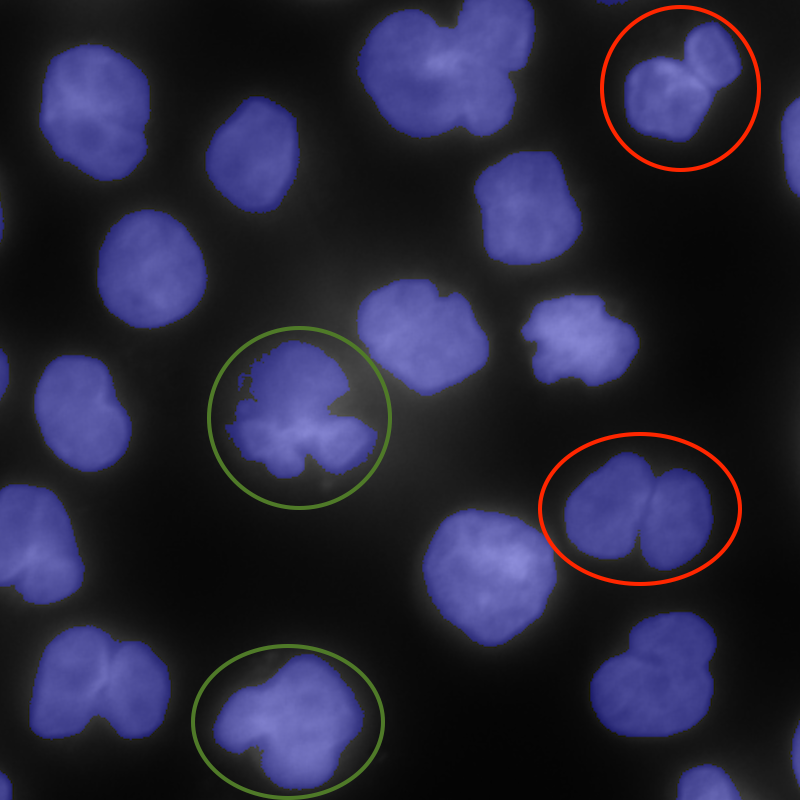
\includegraphics{bilder/close-located-cells/segmented.png}
        \end{tabularx}
    \caption{Closely located cells}
    \label{fig:closely-located-cells}
\end{figure}

\subsubsection{Thresholding}
\begin{figure}[htb]
	\begin{center}
		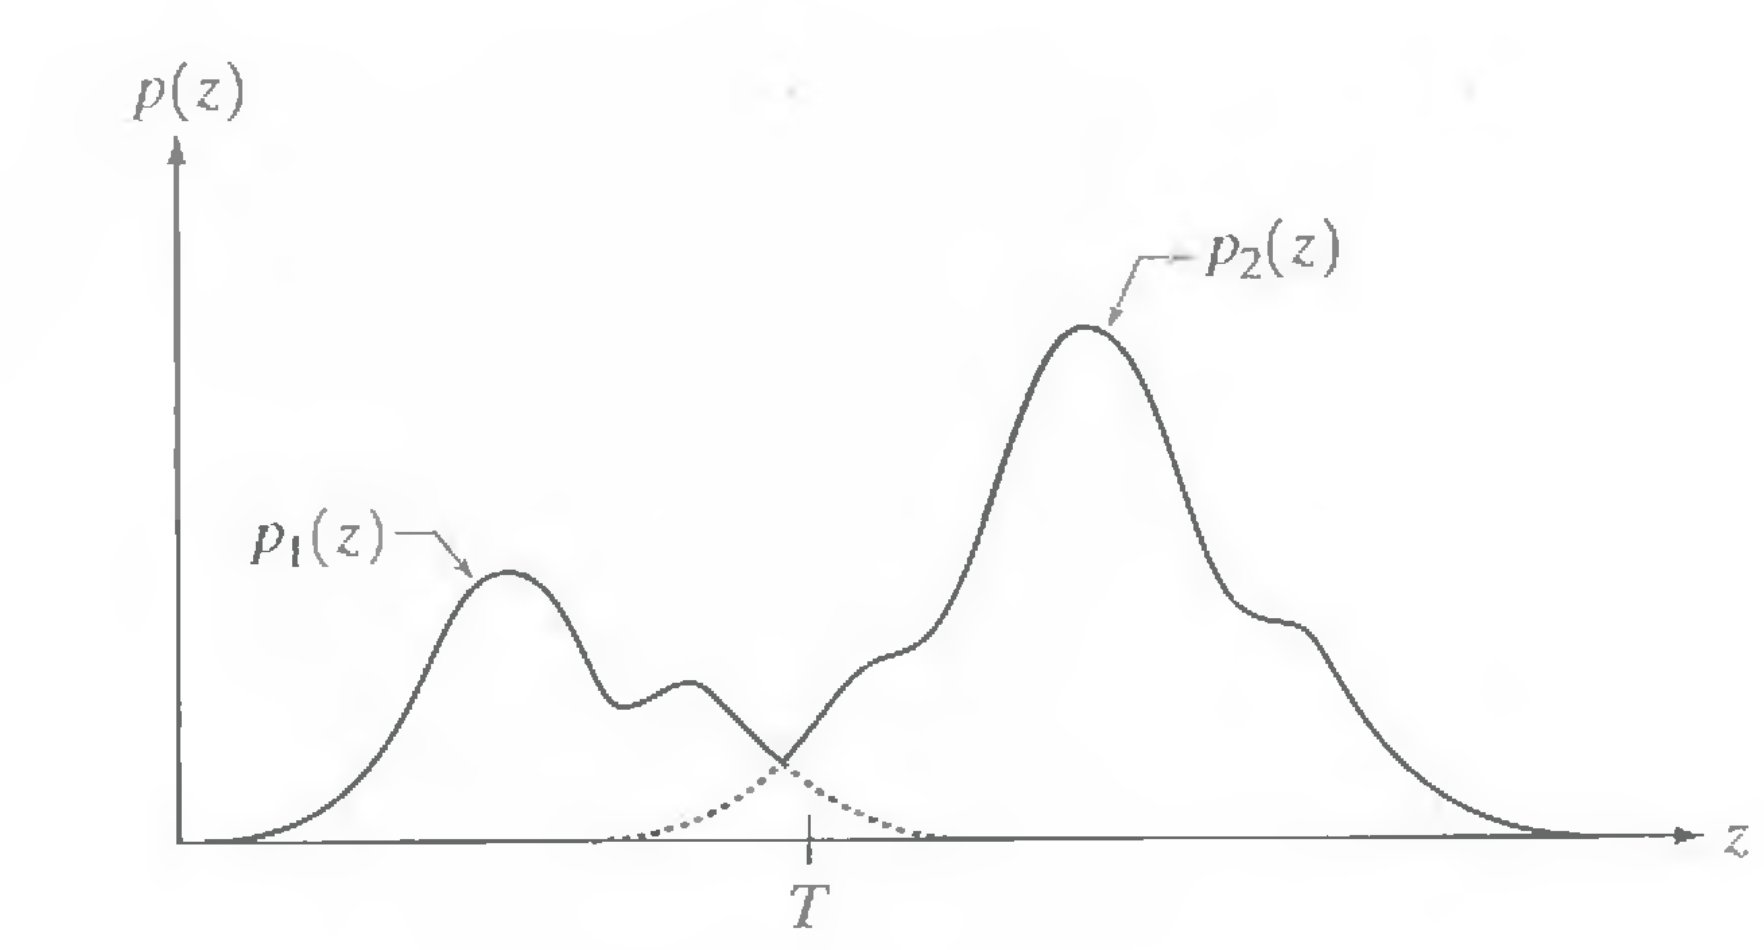
\includegraphics[width=0.8\linewidth]{bilder/Gonzalez.png}
		\caption{Histogram as a probability density function}\label{fig:gmm}
	\end{center}
\end{figure}

\begin{table}
\centering
    \begin{tabular}{||c c||} 
     \hline
     Local Threshold & Global Threshold \\ [0.5ex] 
     \hline\hline
     0.3 sec & 17 sec  \\ 
     \hline
    \end{tabular}
    \caption{Threshold timing}
    \label{tab:threshold-timing}
\end{table}

\begin{figure}[ht] 
    \begin{subfigure}[b]{0.5\linewidth}
      \centering
      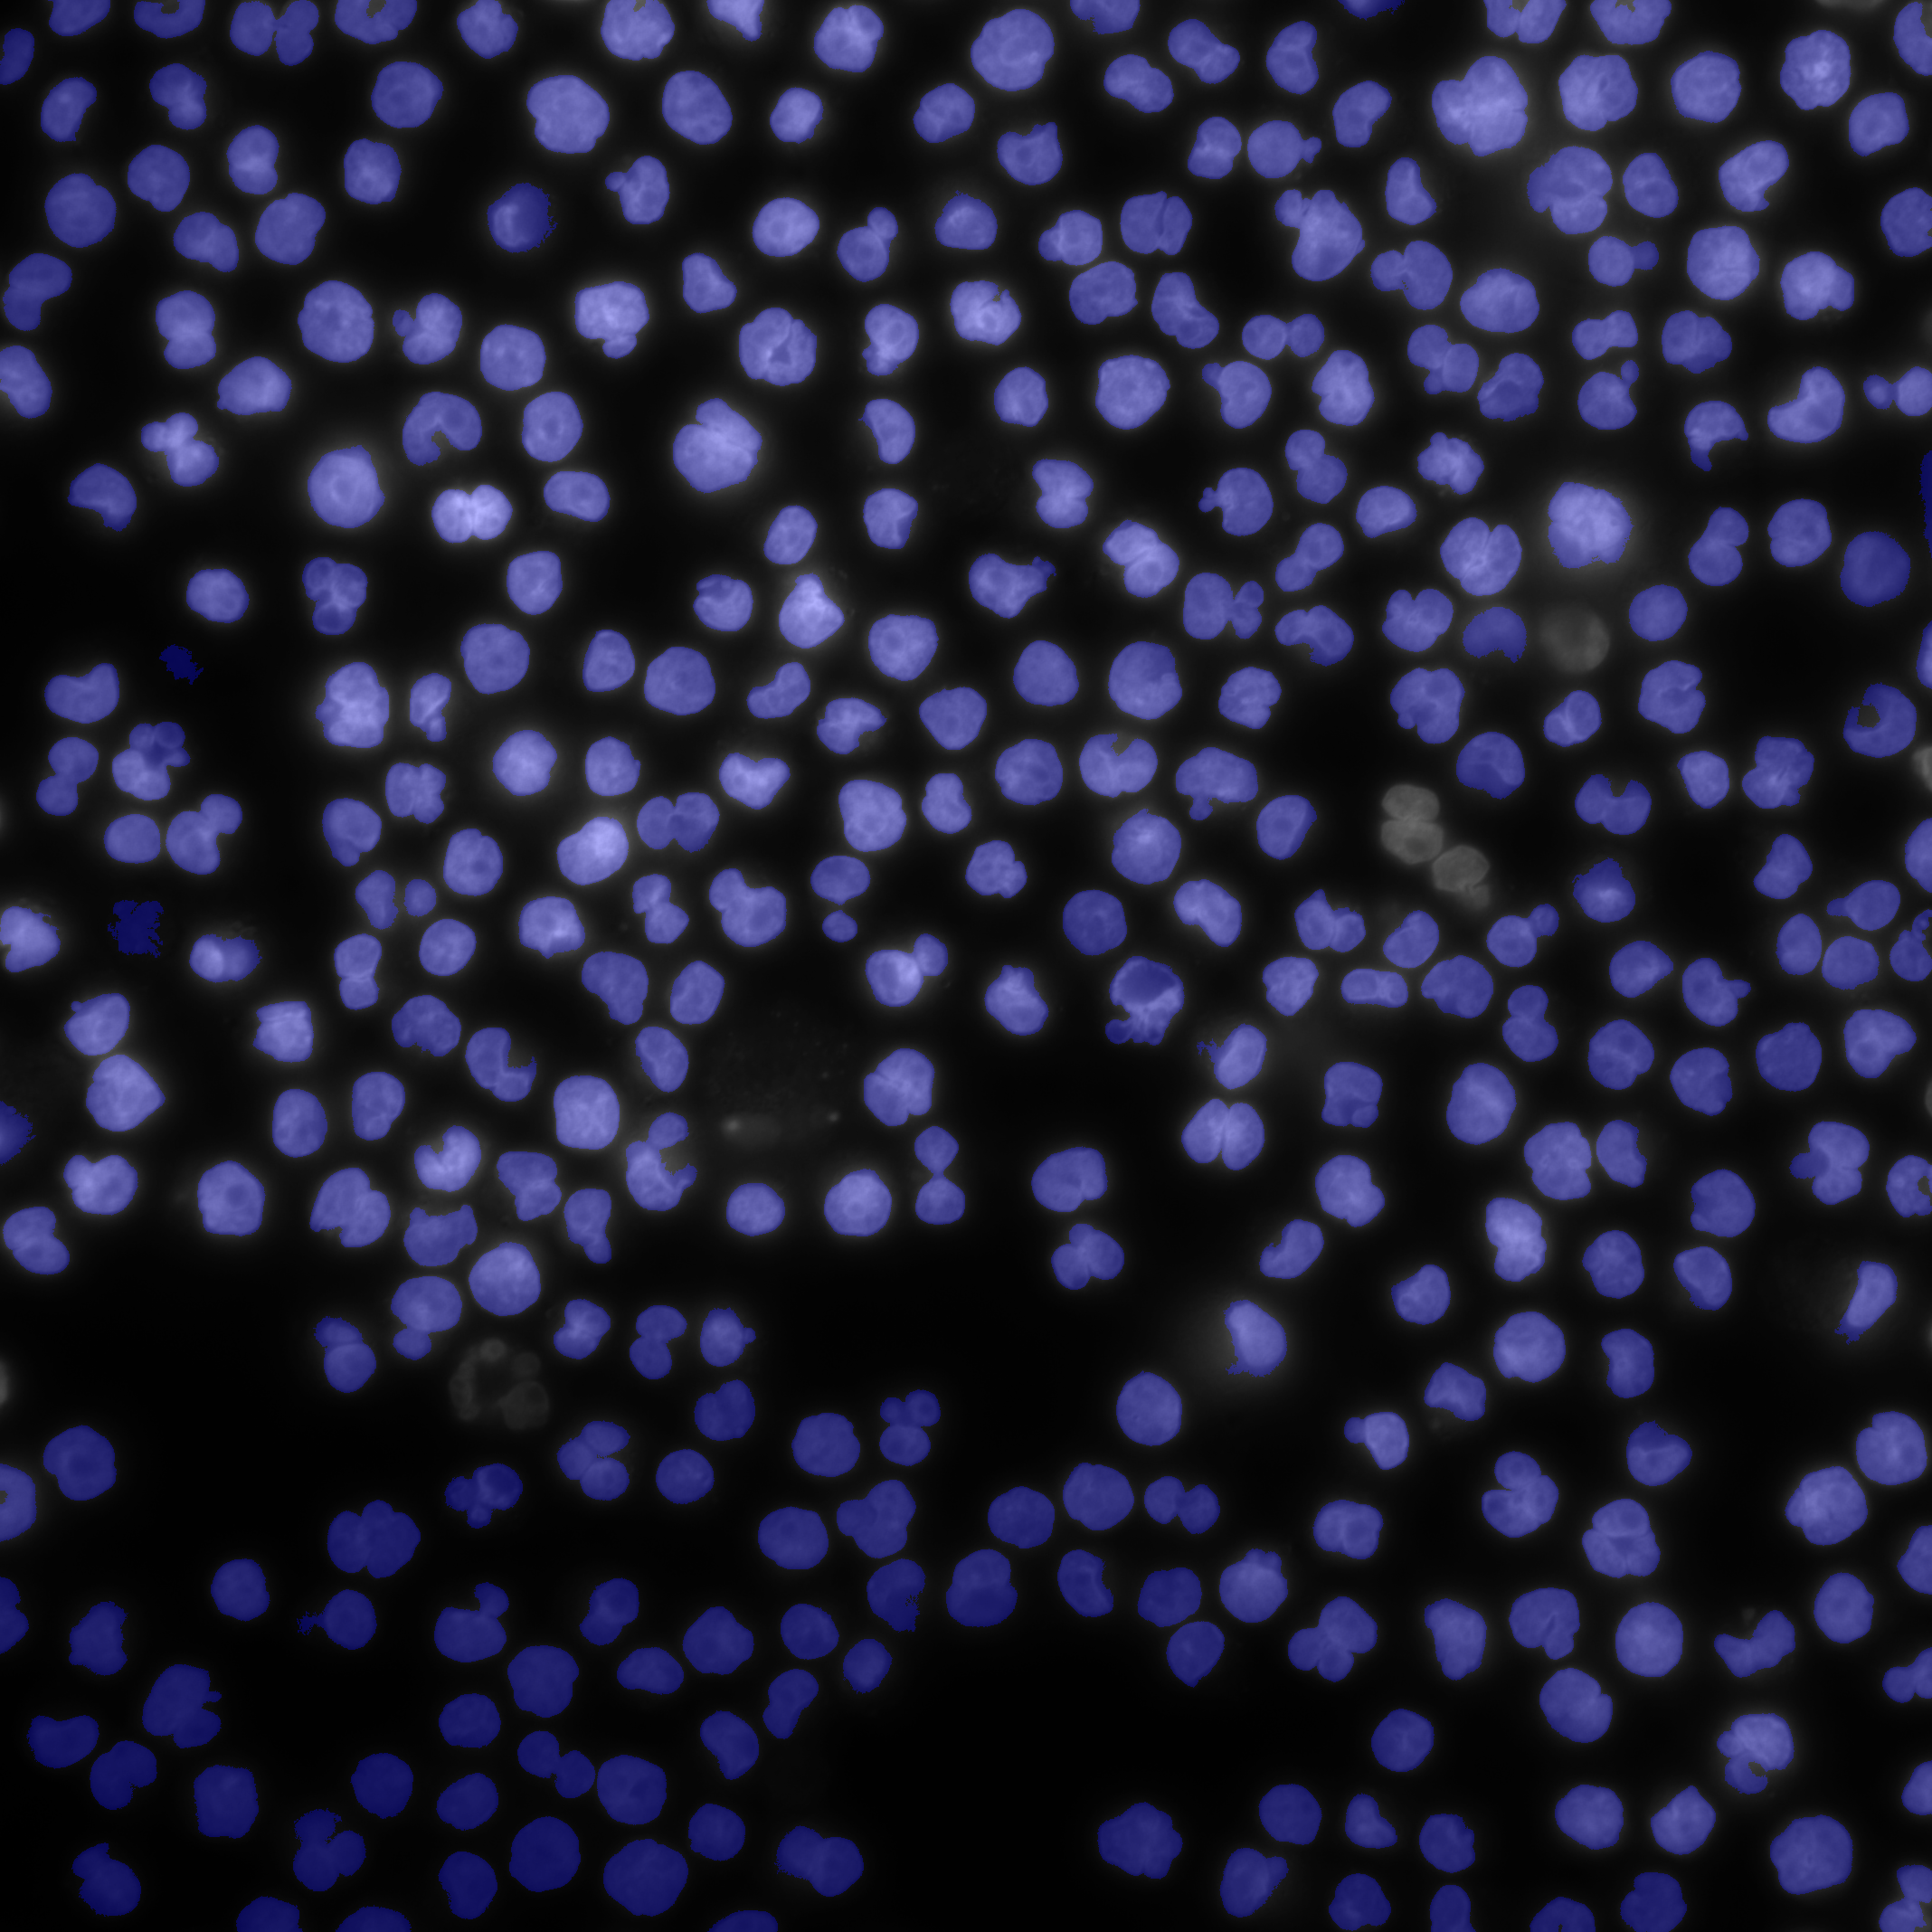
\includegraphics[width=0.75\linewidth]{bilder/difficult-lightning/gradient_local.png} 
      \caption{Local} 
      \label{fig7:a} 
      \vspace{4ex}
    \end{subfigure}%% 
    \begin{subfigure}[b]{0.5\linewidth}
      \centering
      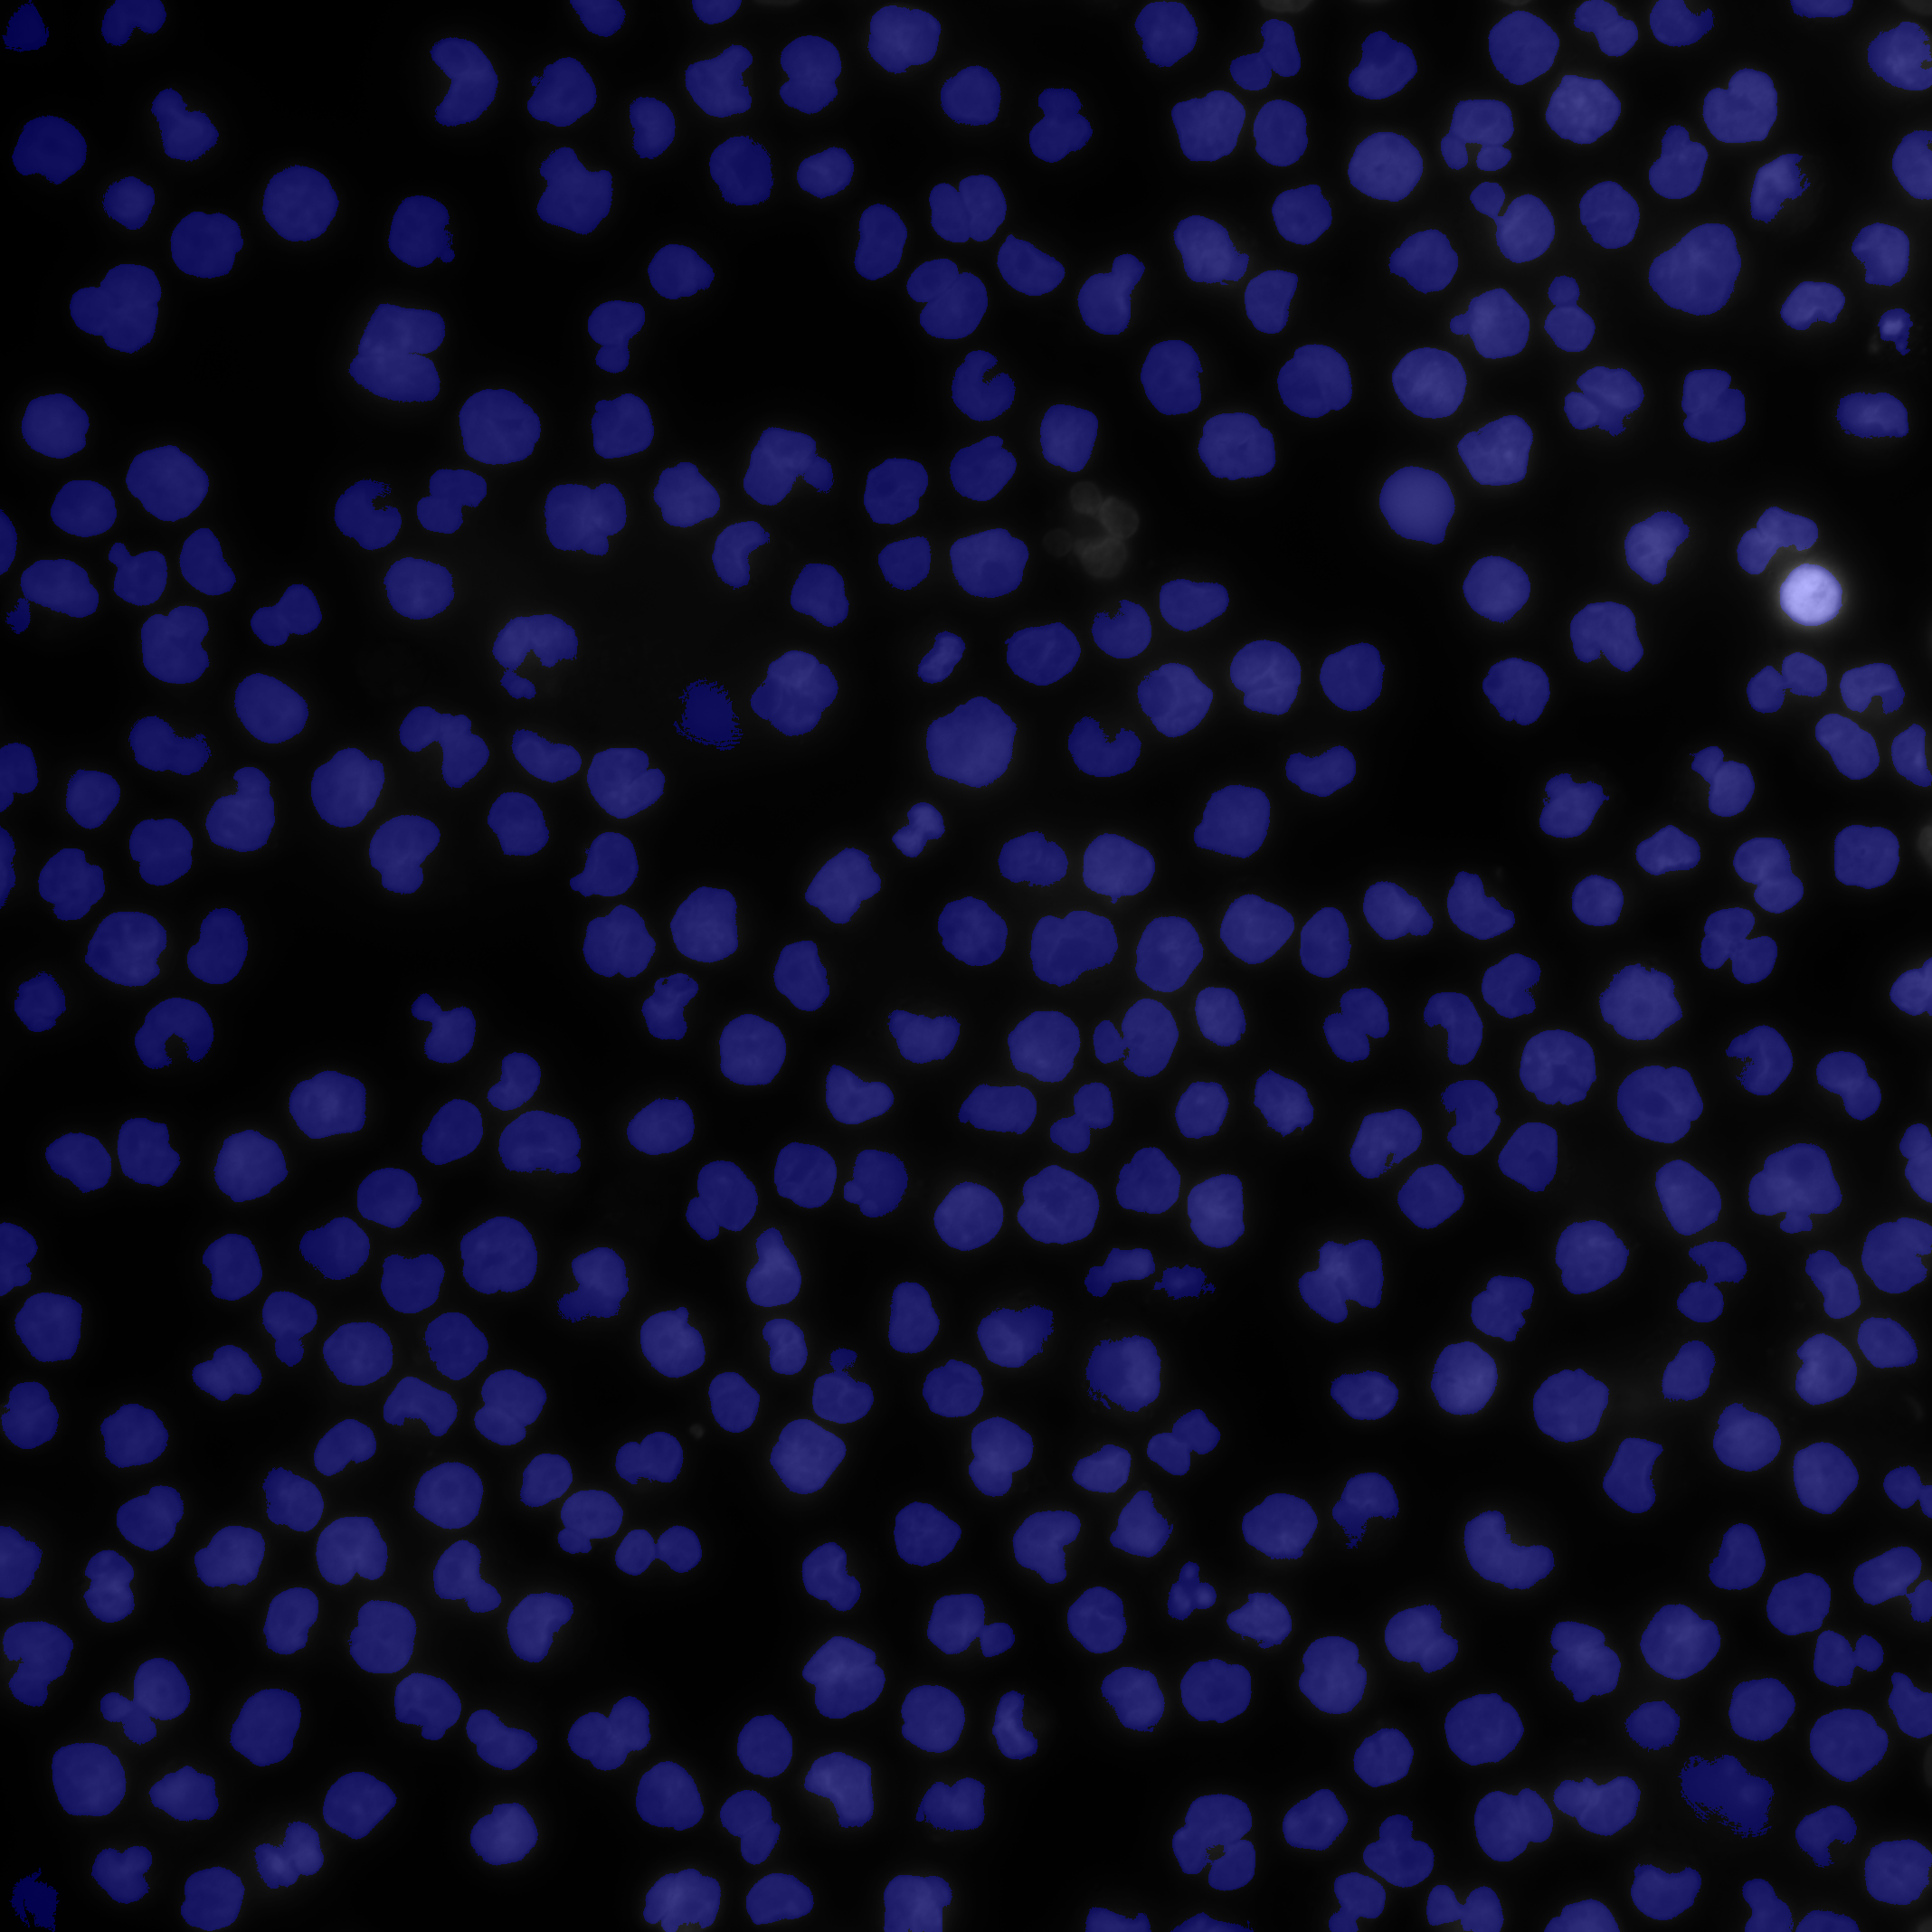
\includegraphics[width=0.75\linewidth]{bilder/difficult-lightning/point_local.png} 
      \caption{Local} 
      \label{fig7:b} 
      \vspace{4ex}
    \end{subfigure} 
    \begin{subfigure}[b]{0.5\linewidth}
      \centering
      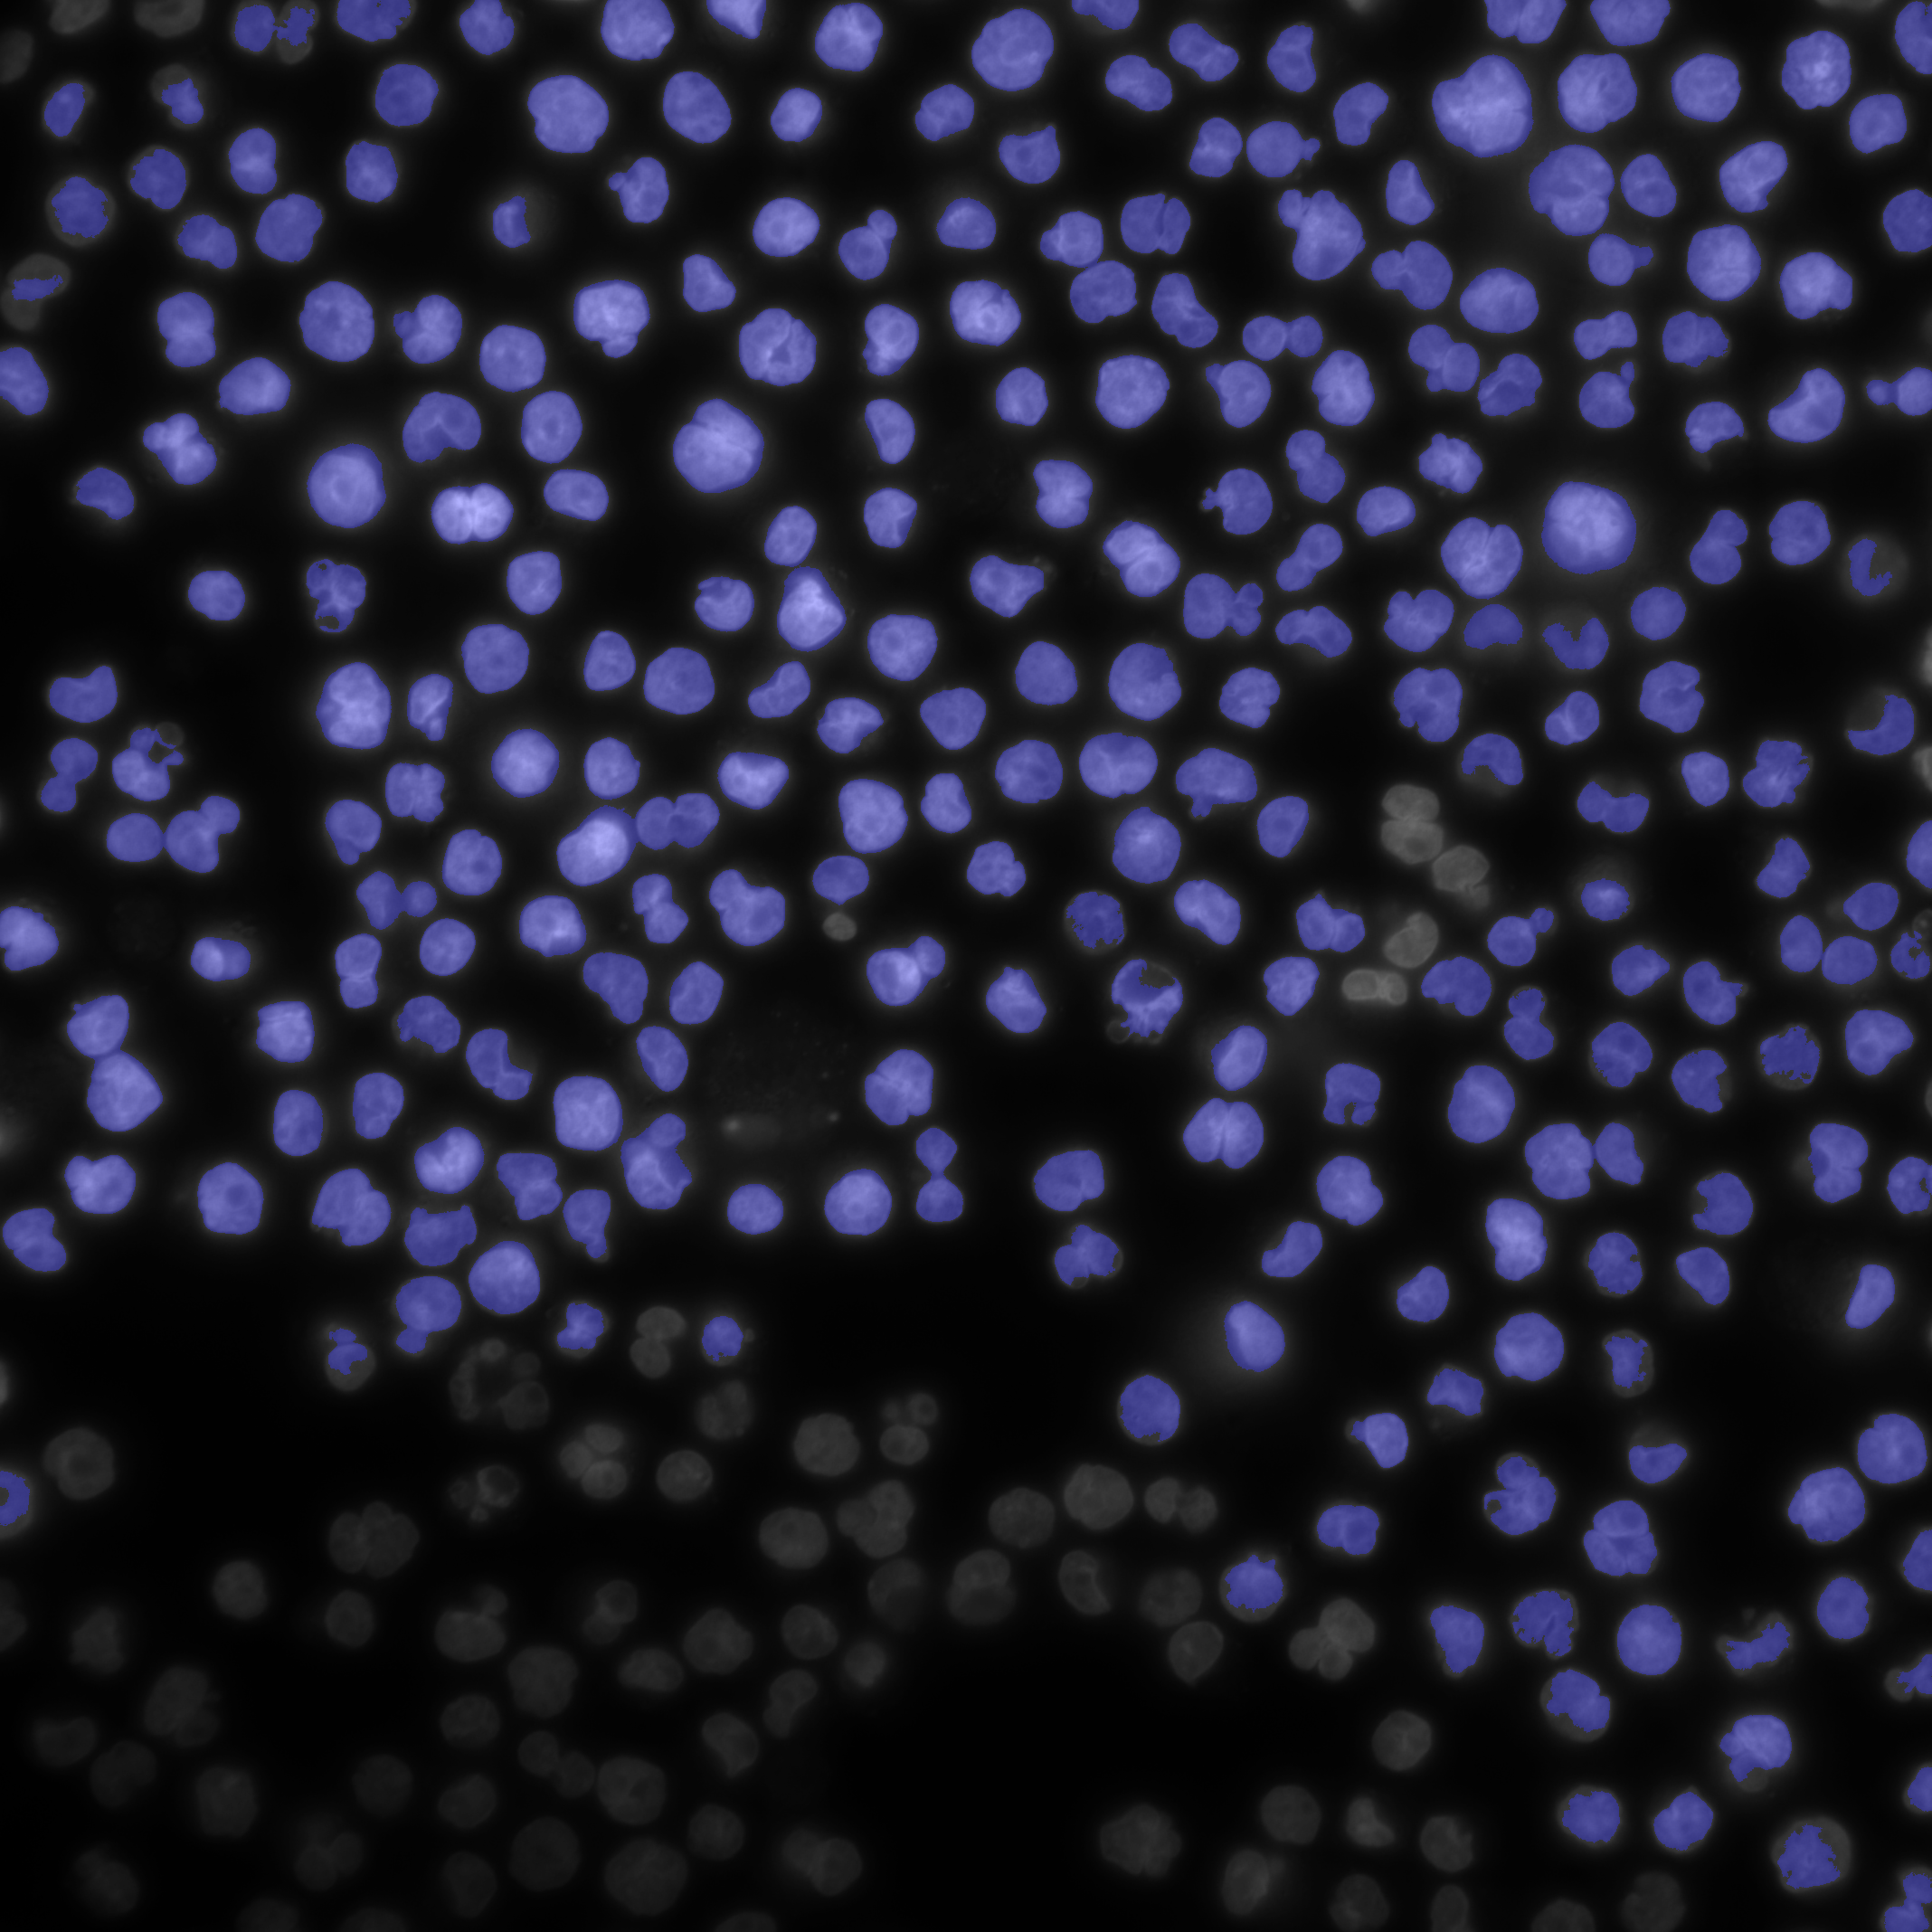
\includegraphics[width=0.75\linewidth]{bilder/difficult-lightning/gradient_min.png} 
      \caption{Global, minimum} 
      \label{fig7:c} 
    \end{subfigure}%%
    \begin{subfigure}[b]{0.5\linewidth}
      \centering
      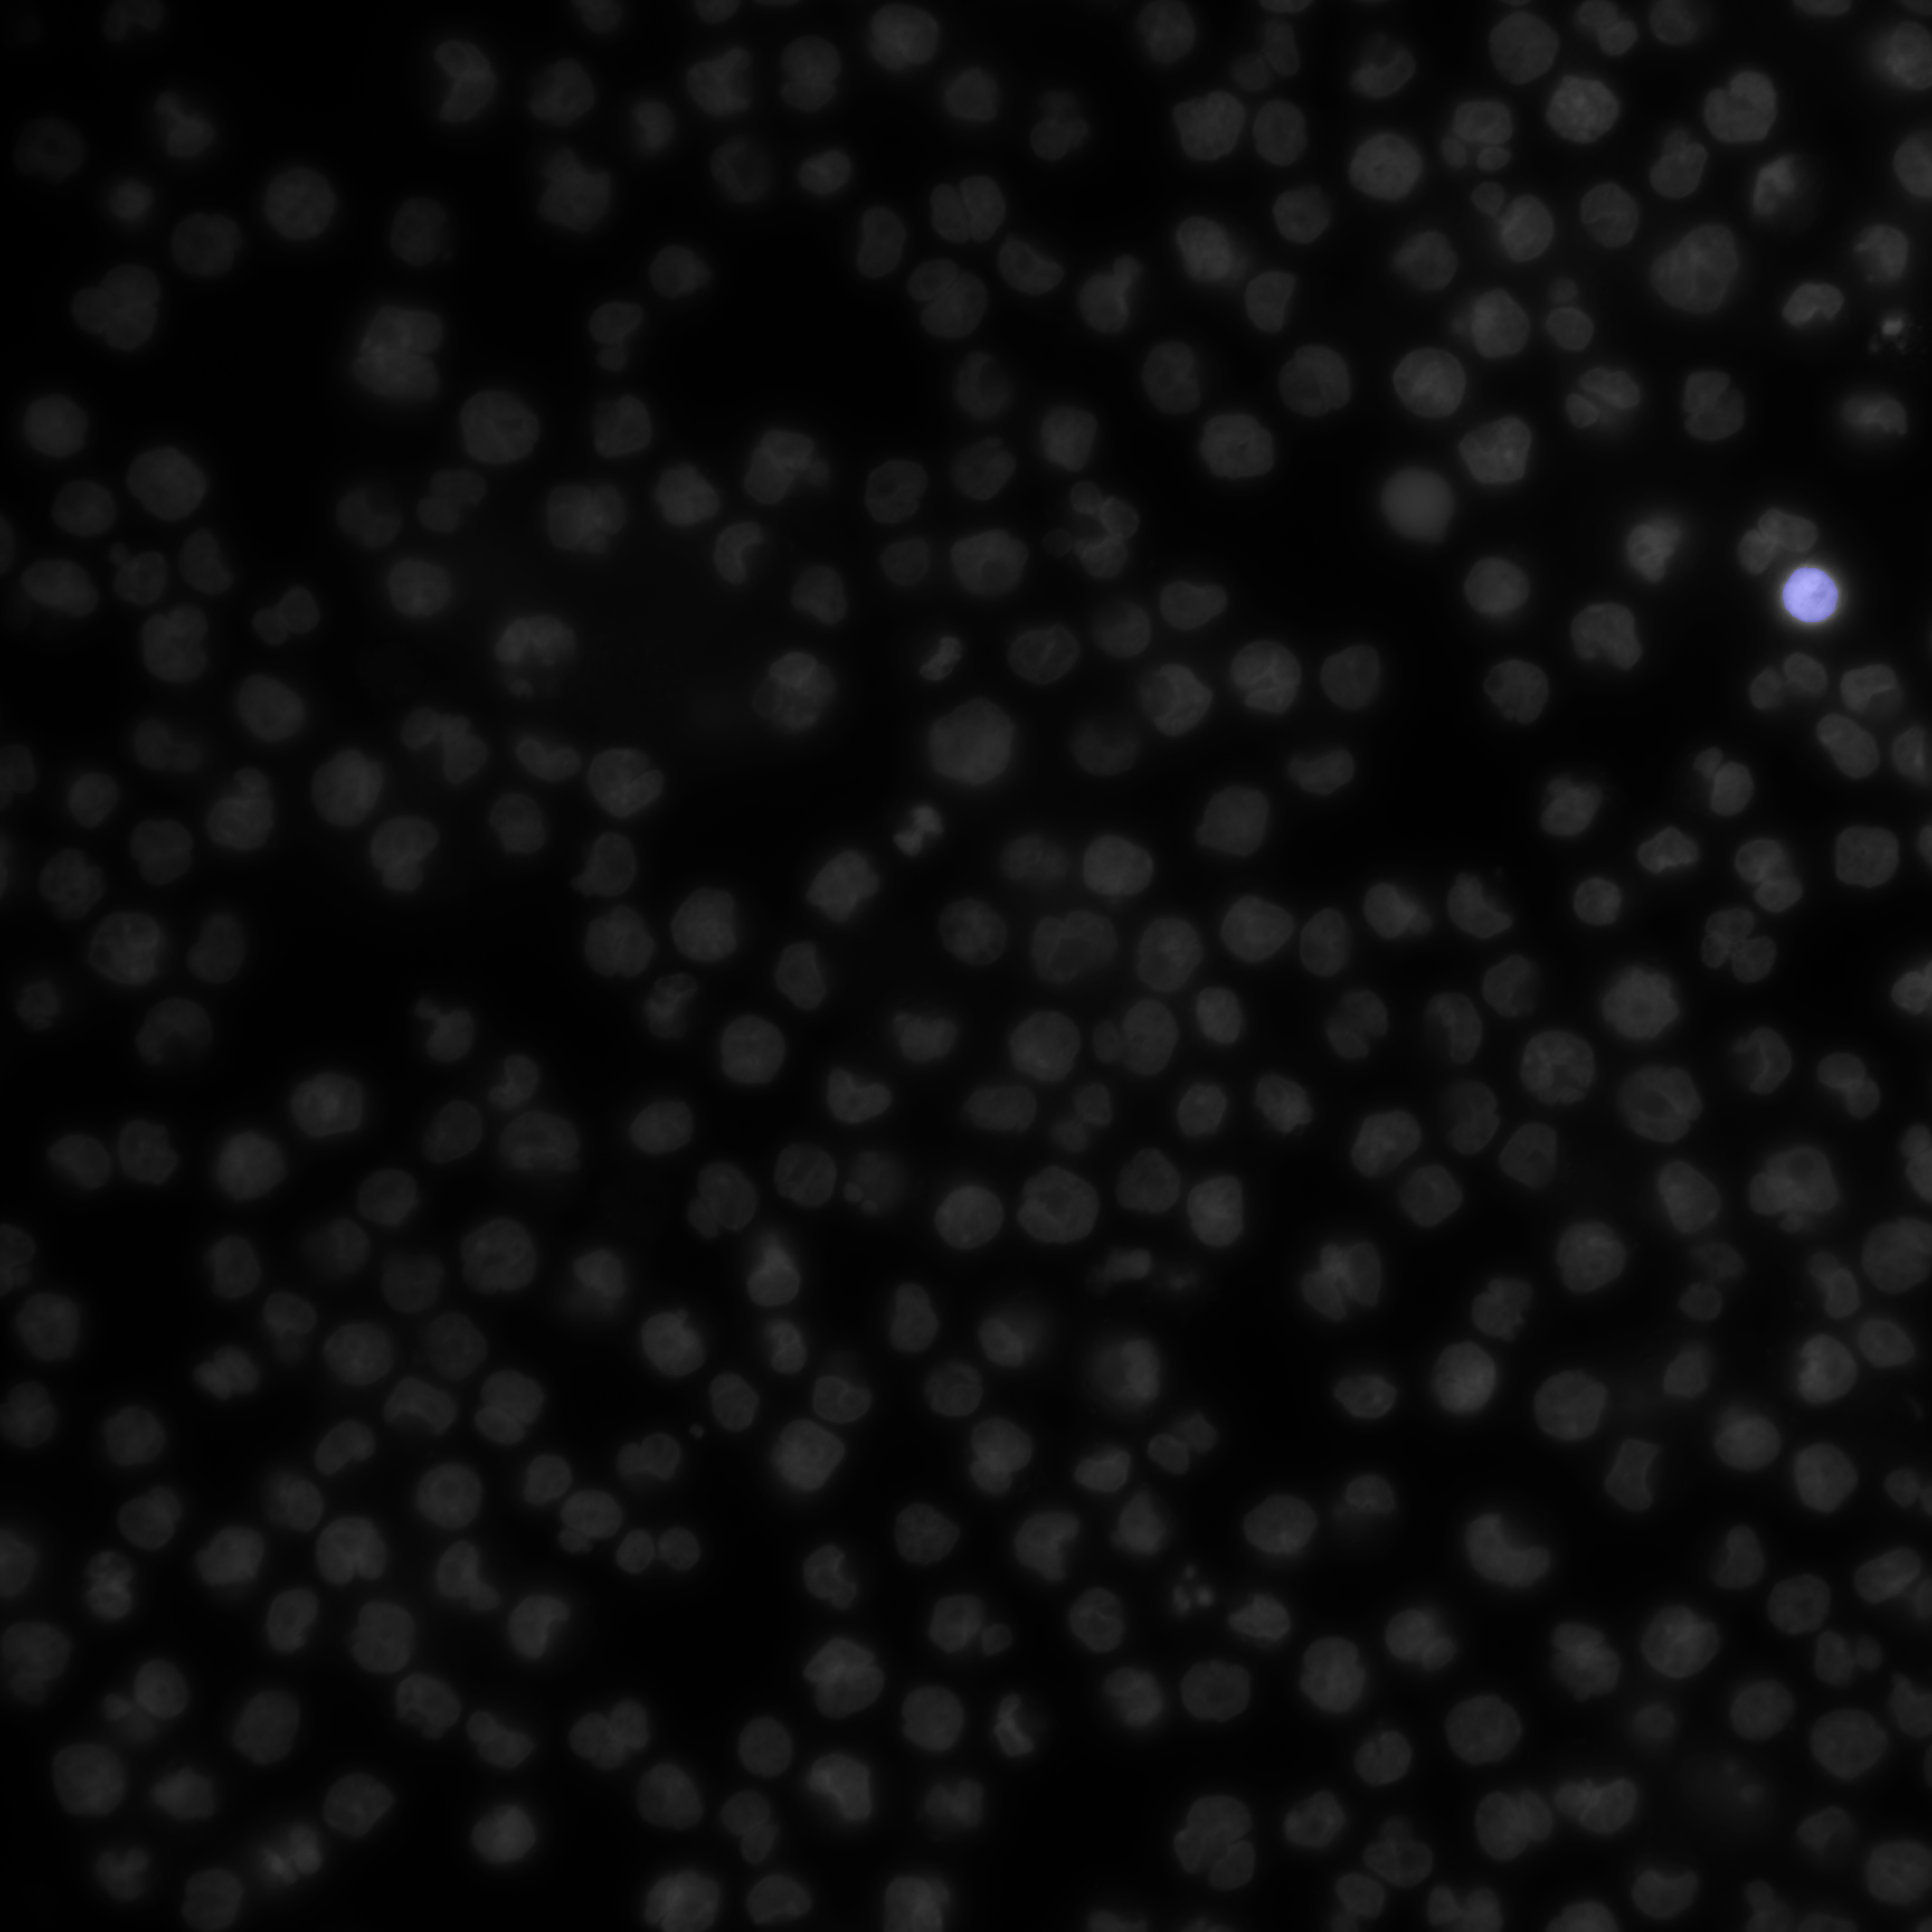
\includegraphics[width=0.75\linewidth]{bilder/difficult-lightning/point_min.png} 
      \caption{Global, minimum} 
      \label{fig7:d} 
    \end{subfigure} 
    \caption{Local vs. Global thresholding}
    \label{fig7} 
\end{figure}

\begin{figure}[H]
    \centering
    \setkeys{Gin}{width=\linewidth}
    \centering
        \begin{tabularx}{\textwidth}{YY}
            \textbf{Local thresholding} &
            \textbf{Minimum thresholding} \\
            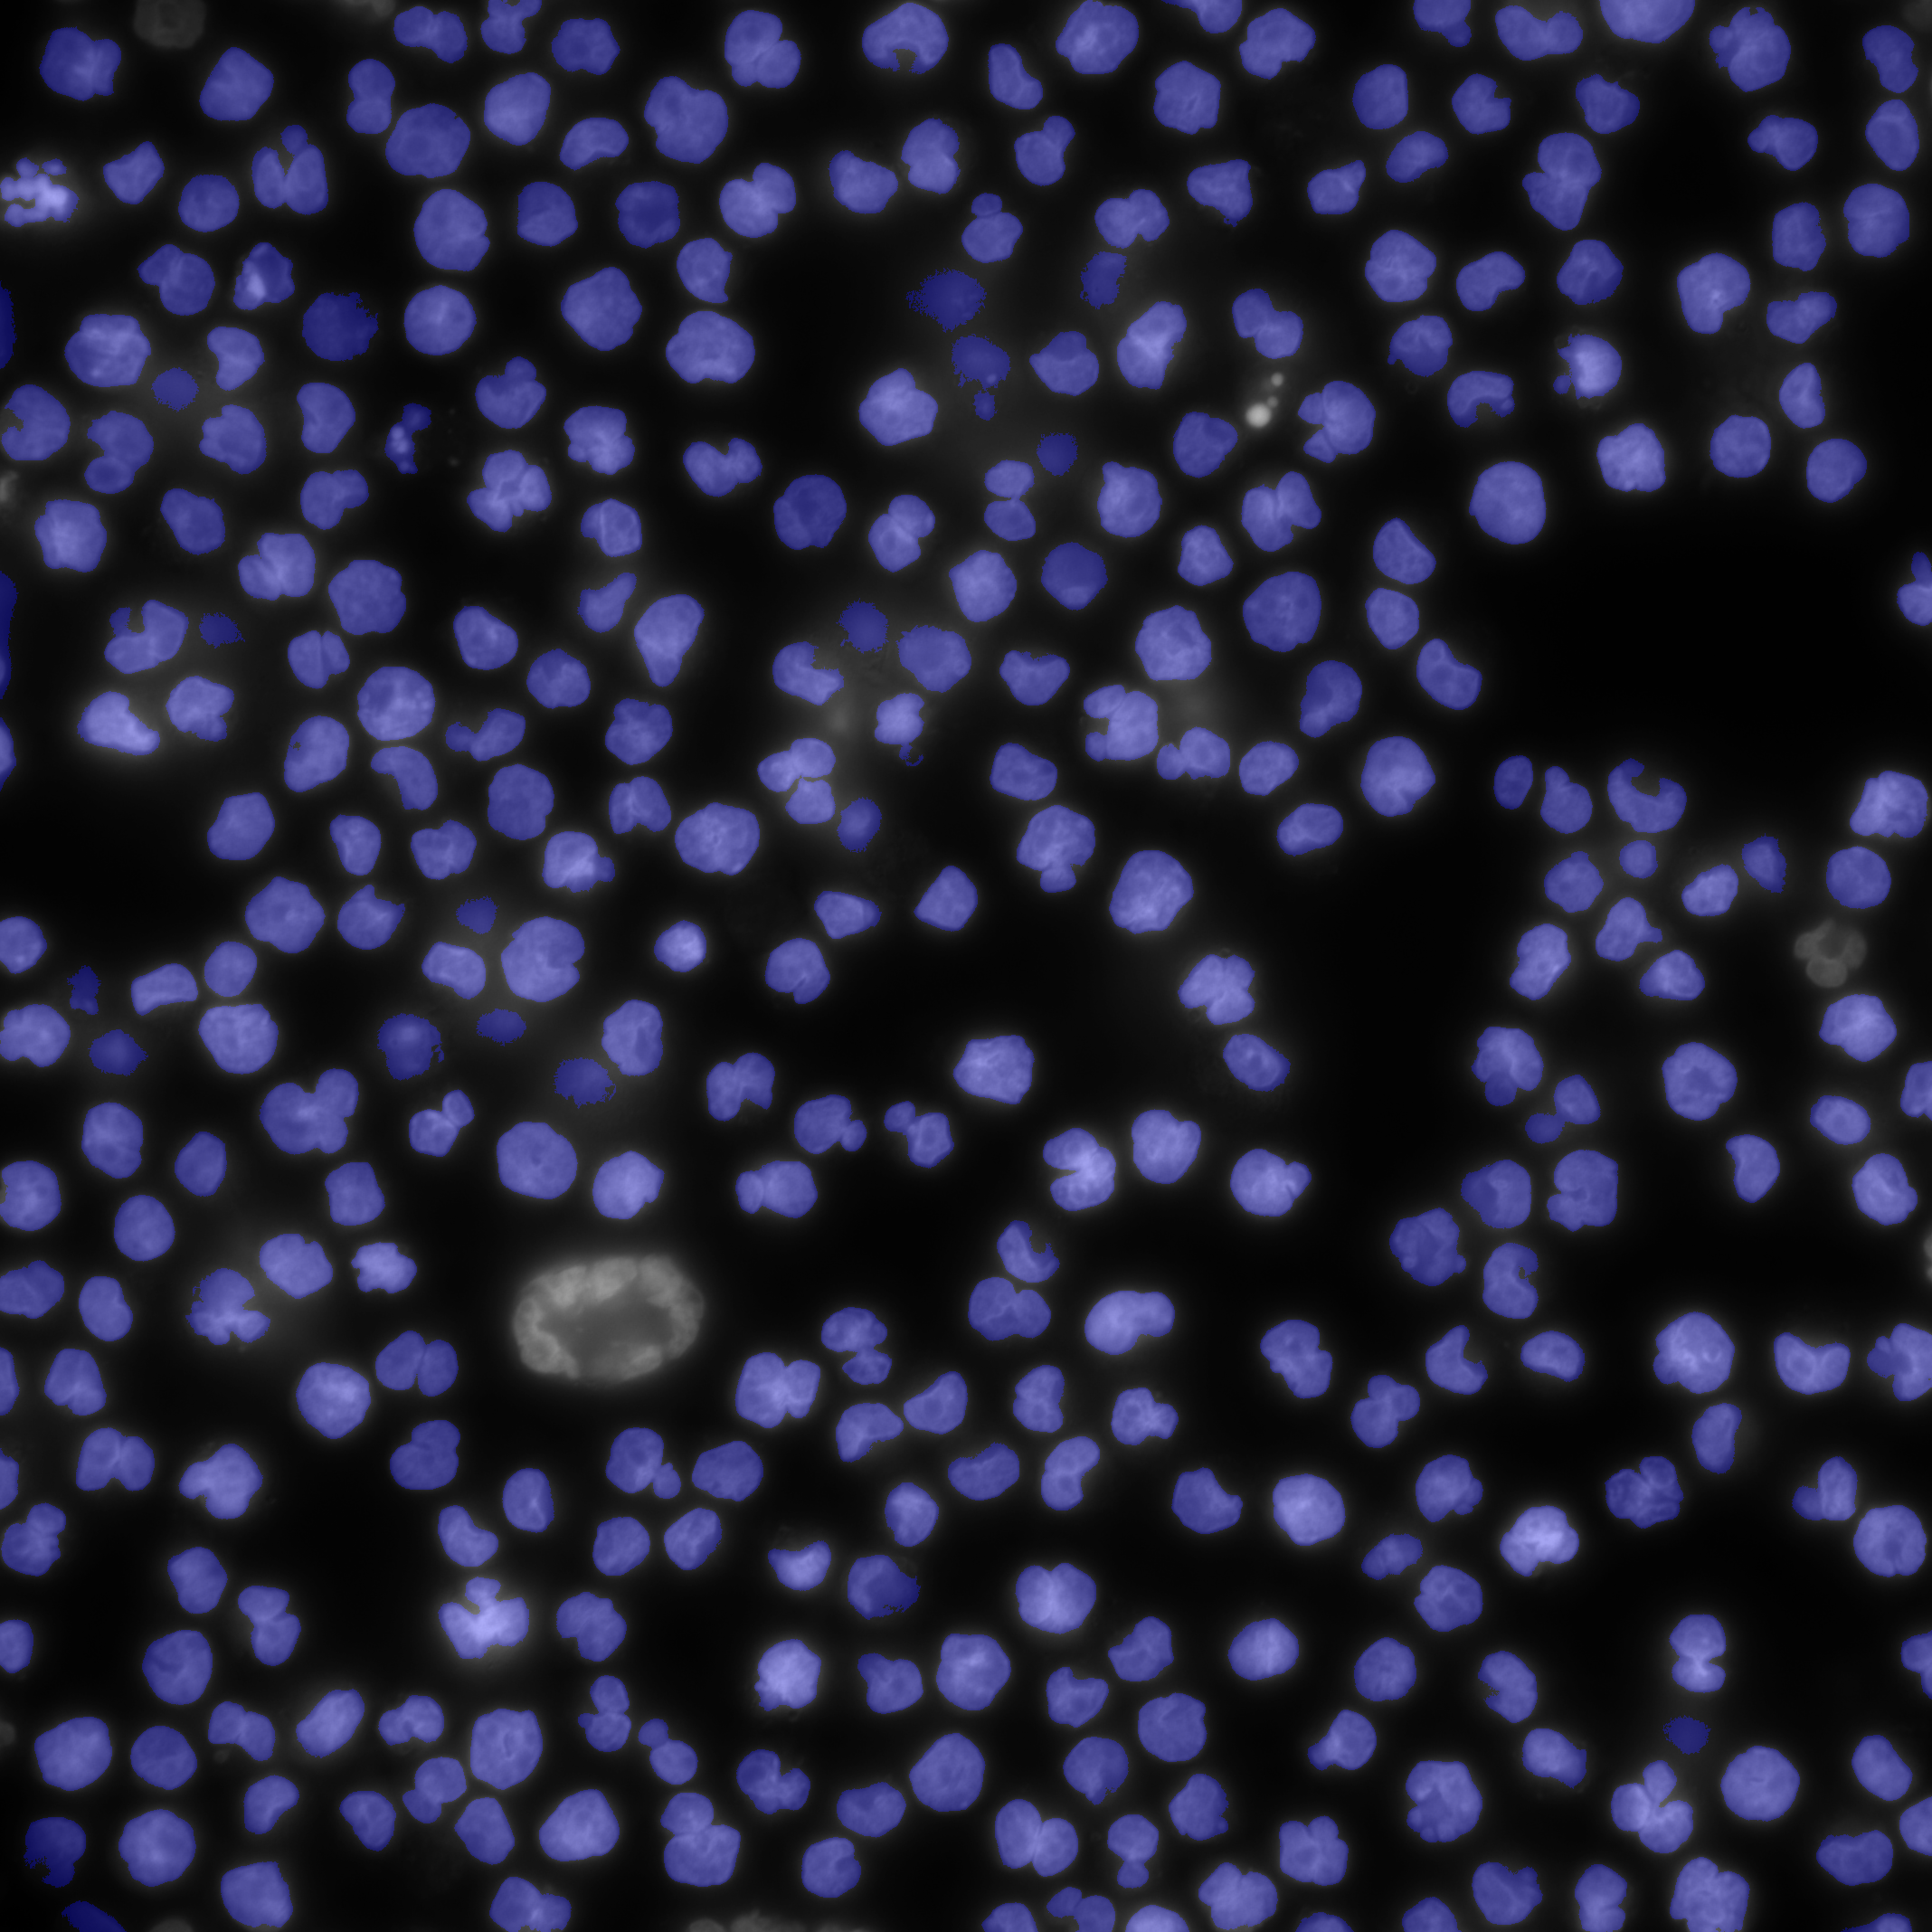
\includegraphics{bilder/difficult-lightning/normal_local.png} & 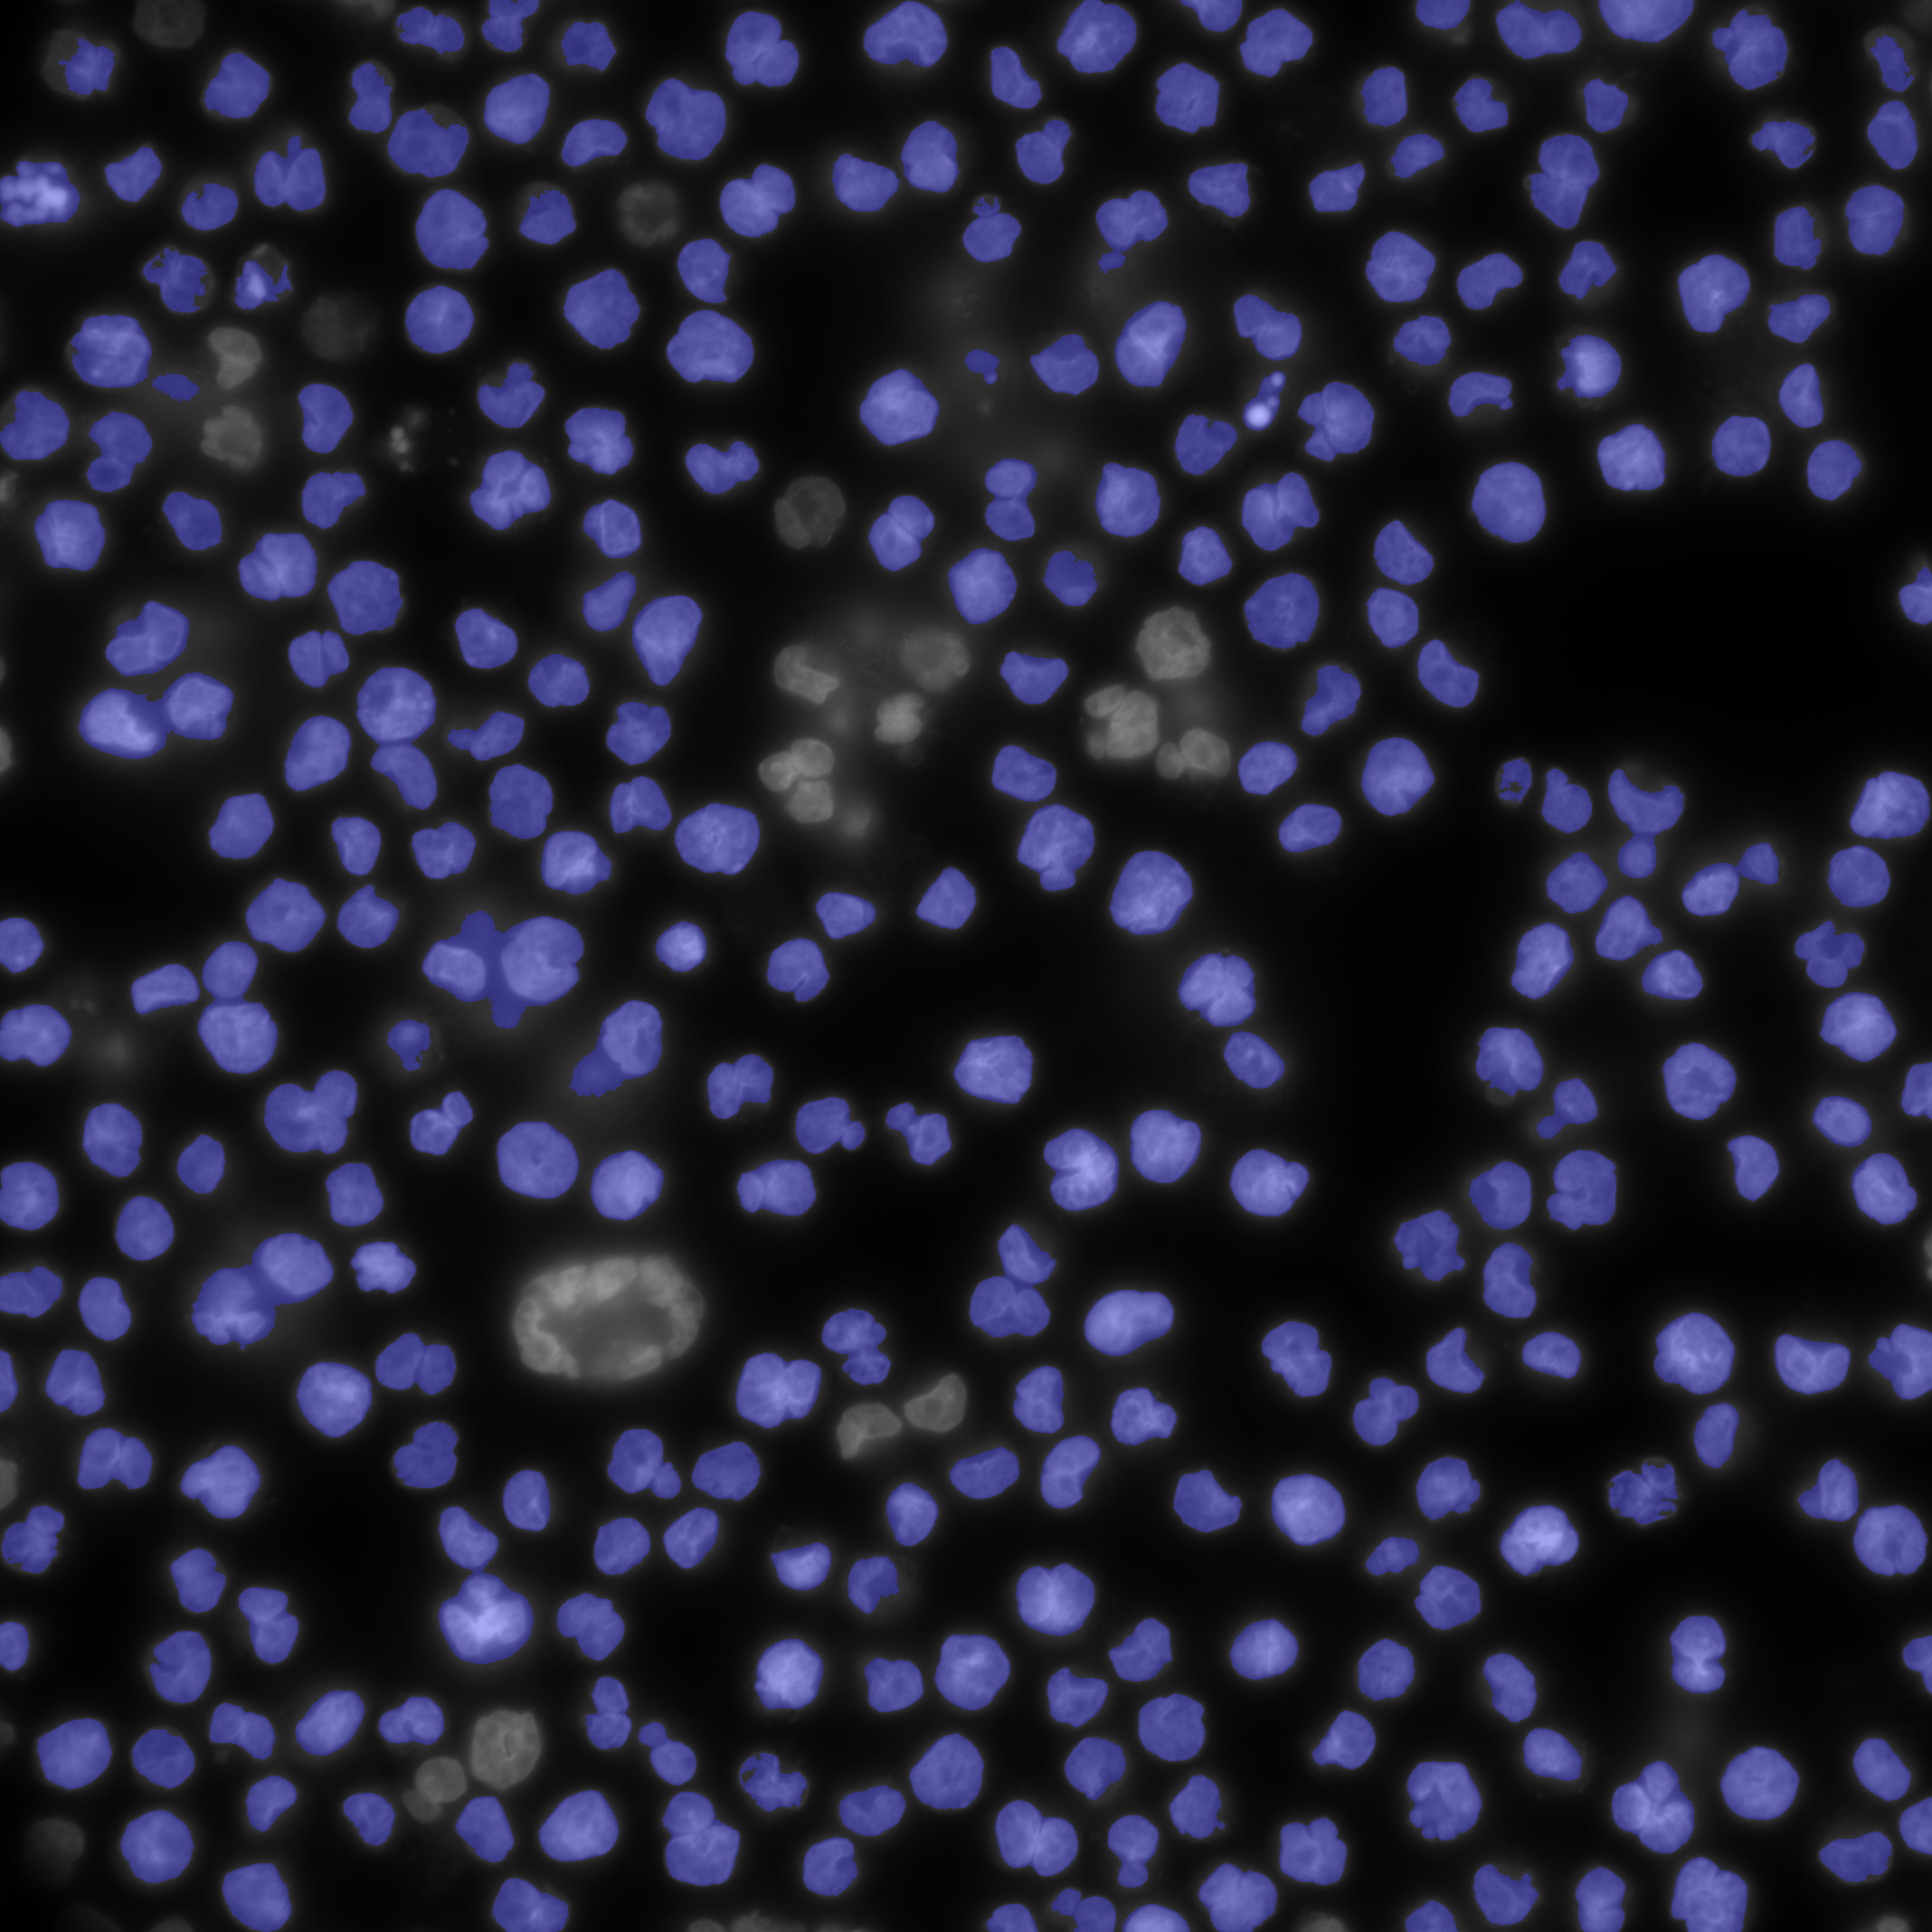
\includegraphics{bilder/difficult-lightning/normal_min.png}
        \end{tabularx}
    \caption{Local vs. Global thresholding (normal conditions)}
    \label{fig:local-vs-global-normal}
\end{figure}

\subsubsection{Overall algorithm}

\begin{figure}[H]
    \centering
    \setkeys{Gin}{width=\linewidth}
    \centering
        \begin{tabularx}{\textwidth}{YYYY}
            \textbf{Normalized input} &
            \textbf{Local threshold} &
            \textbf{Filled holes} &
            \textbf{Filtered regions} \\
            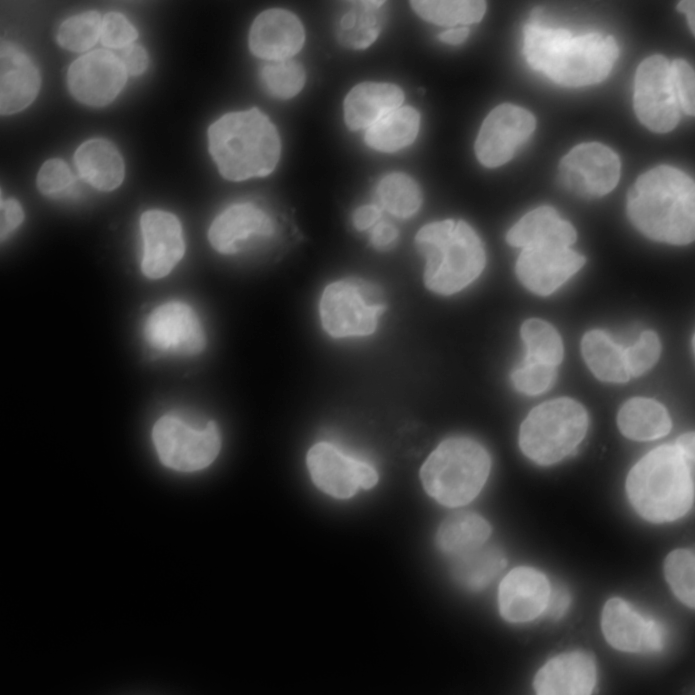
\includegraphics{bilder/segmentation/nuclei-mask/normalized.png} & 
\includegraphics{bilder/segmentation/nuclei-mask/binary_local.png} &
            
\includegraphics{bilder/segmentation/nuclei-mask/filled_holes.png} & 
            
\includegraphics{bilder/segmentation/nuclei-mask/mask.png}
        \end{tabularx}
    \caption{Fluorescence segmentation}
    \label{fig:segmentation-nuclei-steps}
\end{figure}


\subsection{ER-segmentation}

\begin{figure}[H]
    \centering
    \setkeys{Gin}{width=\linewidth}
    \centering
        \begin{tabularx}{\textwidth}{YYYY}
            \textbf{Ground truth} &
            \textbf{Prediction} &
            \textbf{Prediction + nuclei} \\
            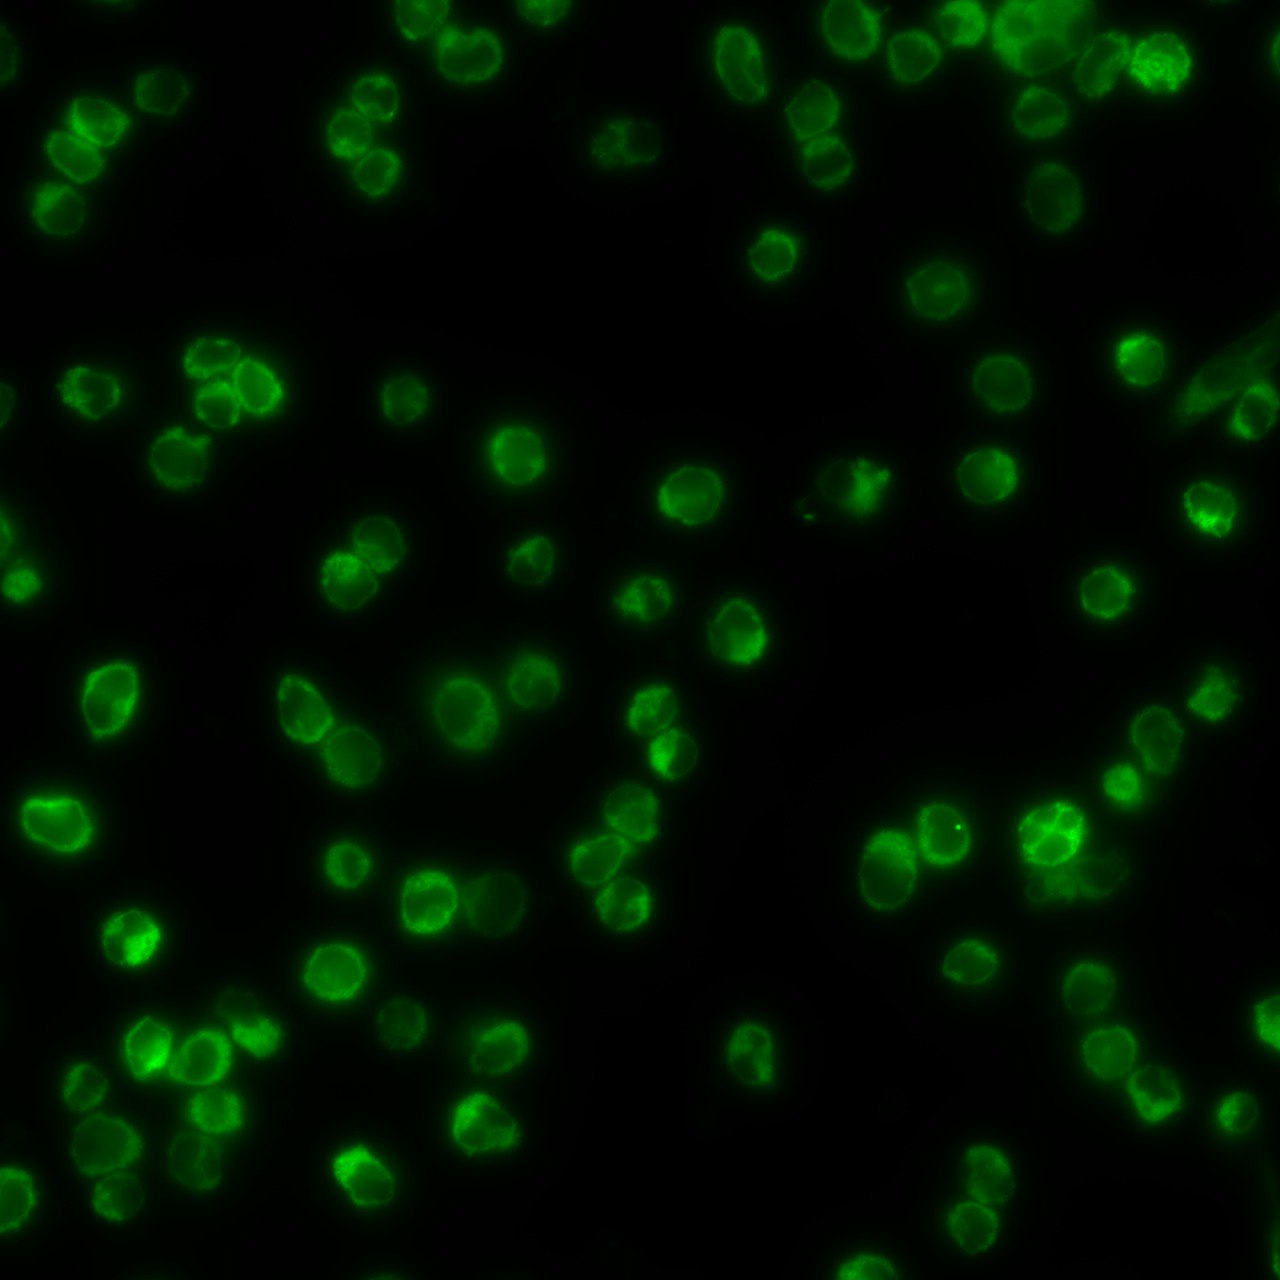
\includegraphics{bilder/ER/gt.jpg} & 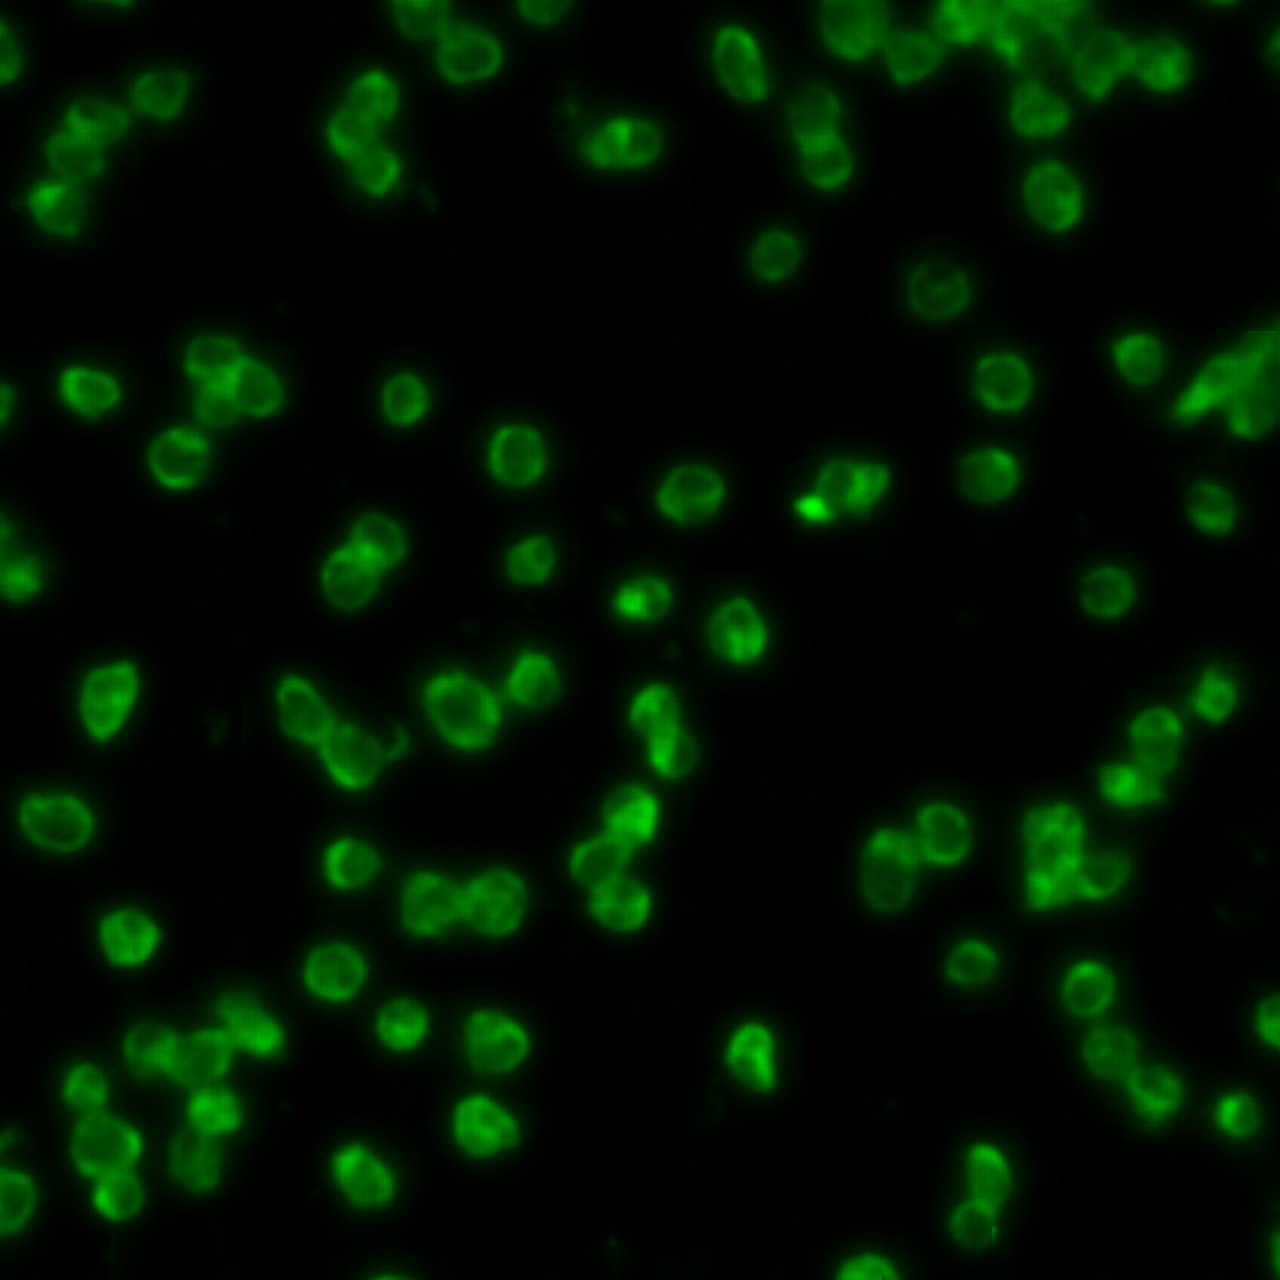
\includegraphics{bilder/ER/er.jpg} &
            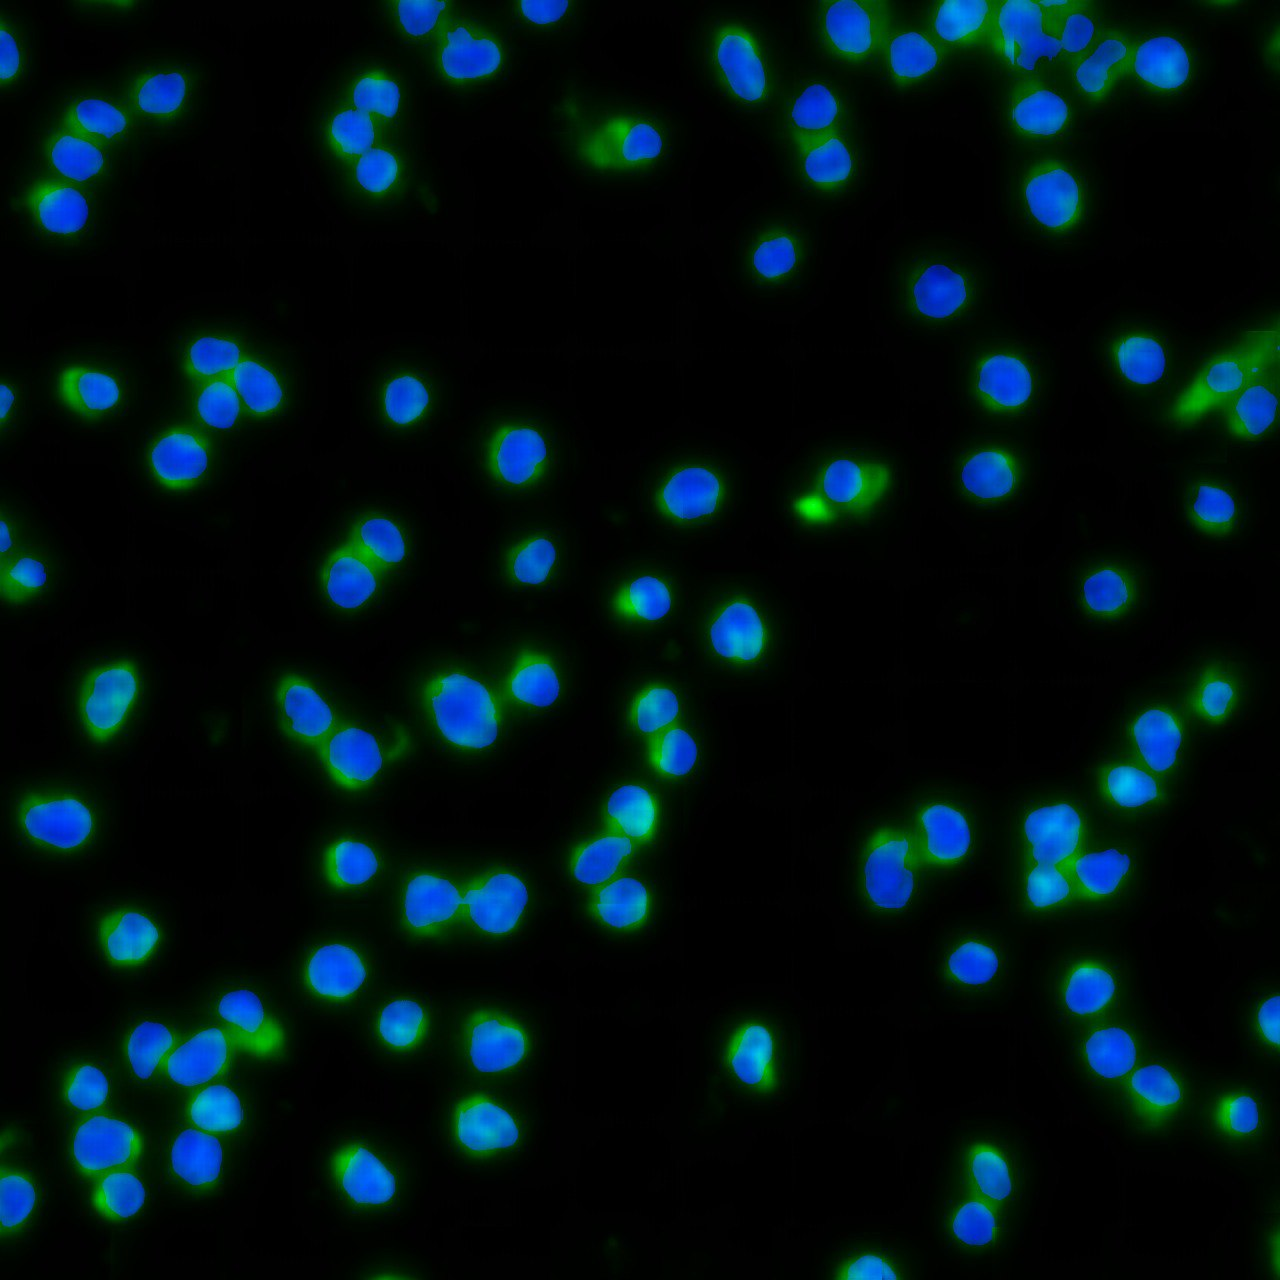
\includegraphics{bilder/ER/gt_nuclei.jpg}
        \end{tabularx}
    \caption{ER prediction}
    \label{fig:er-prediction}
\end{figure}
\begin{figure}[H]
    \centering
    \setkeys{Gin}{width=\linewidth}
    \centering
        \begin{tabularx}{\textwidth}{YYYYYYY}
            \textbf{1} &
            \textbf{2} &
            \textbf{3} &
            \textbf{4} &
            \textbf{5} &
            \textbf{6} &
            \textbf{7} \\
            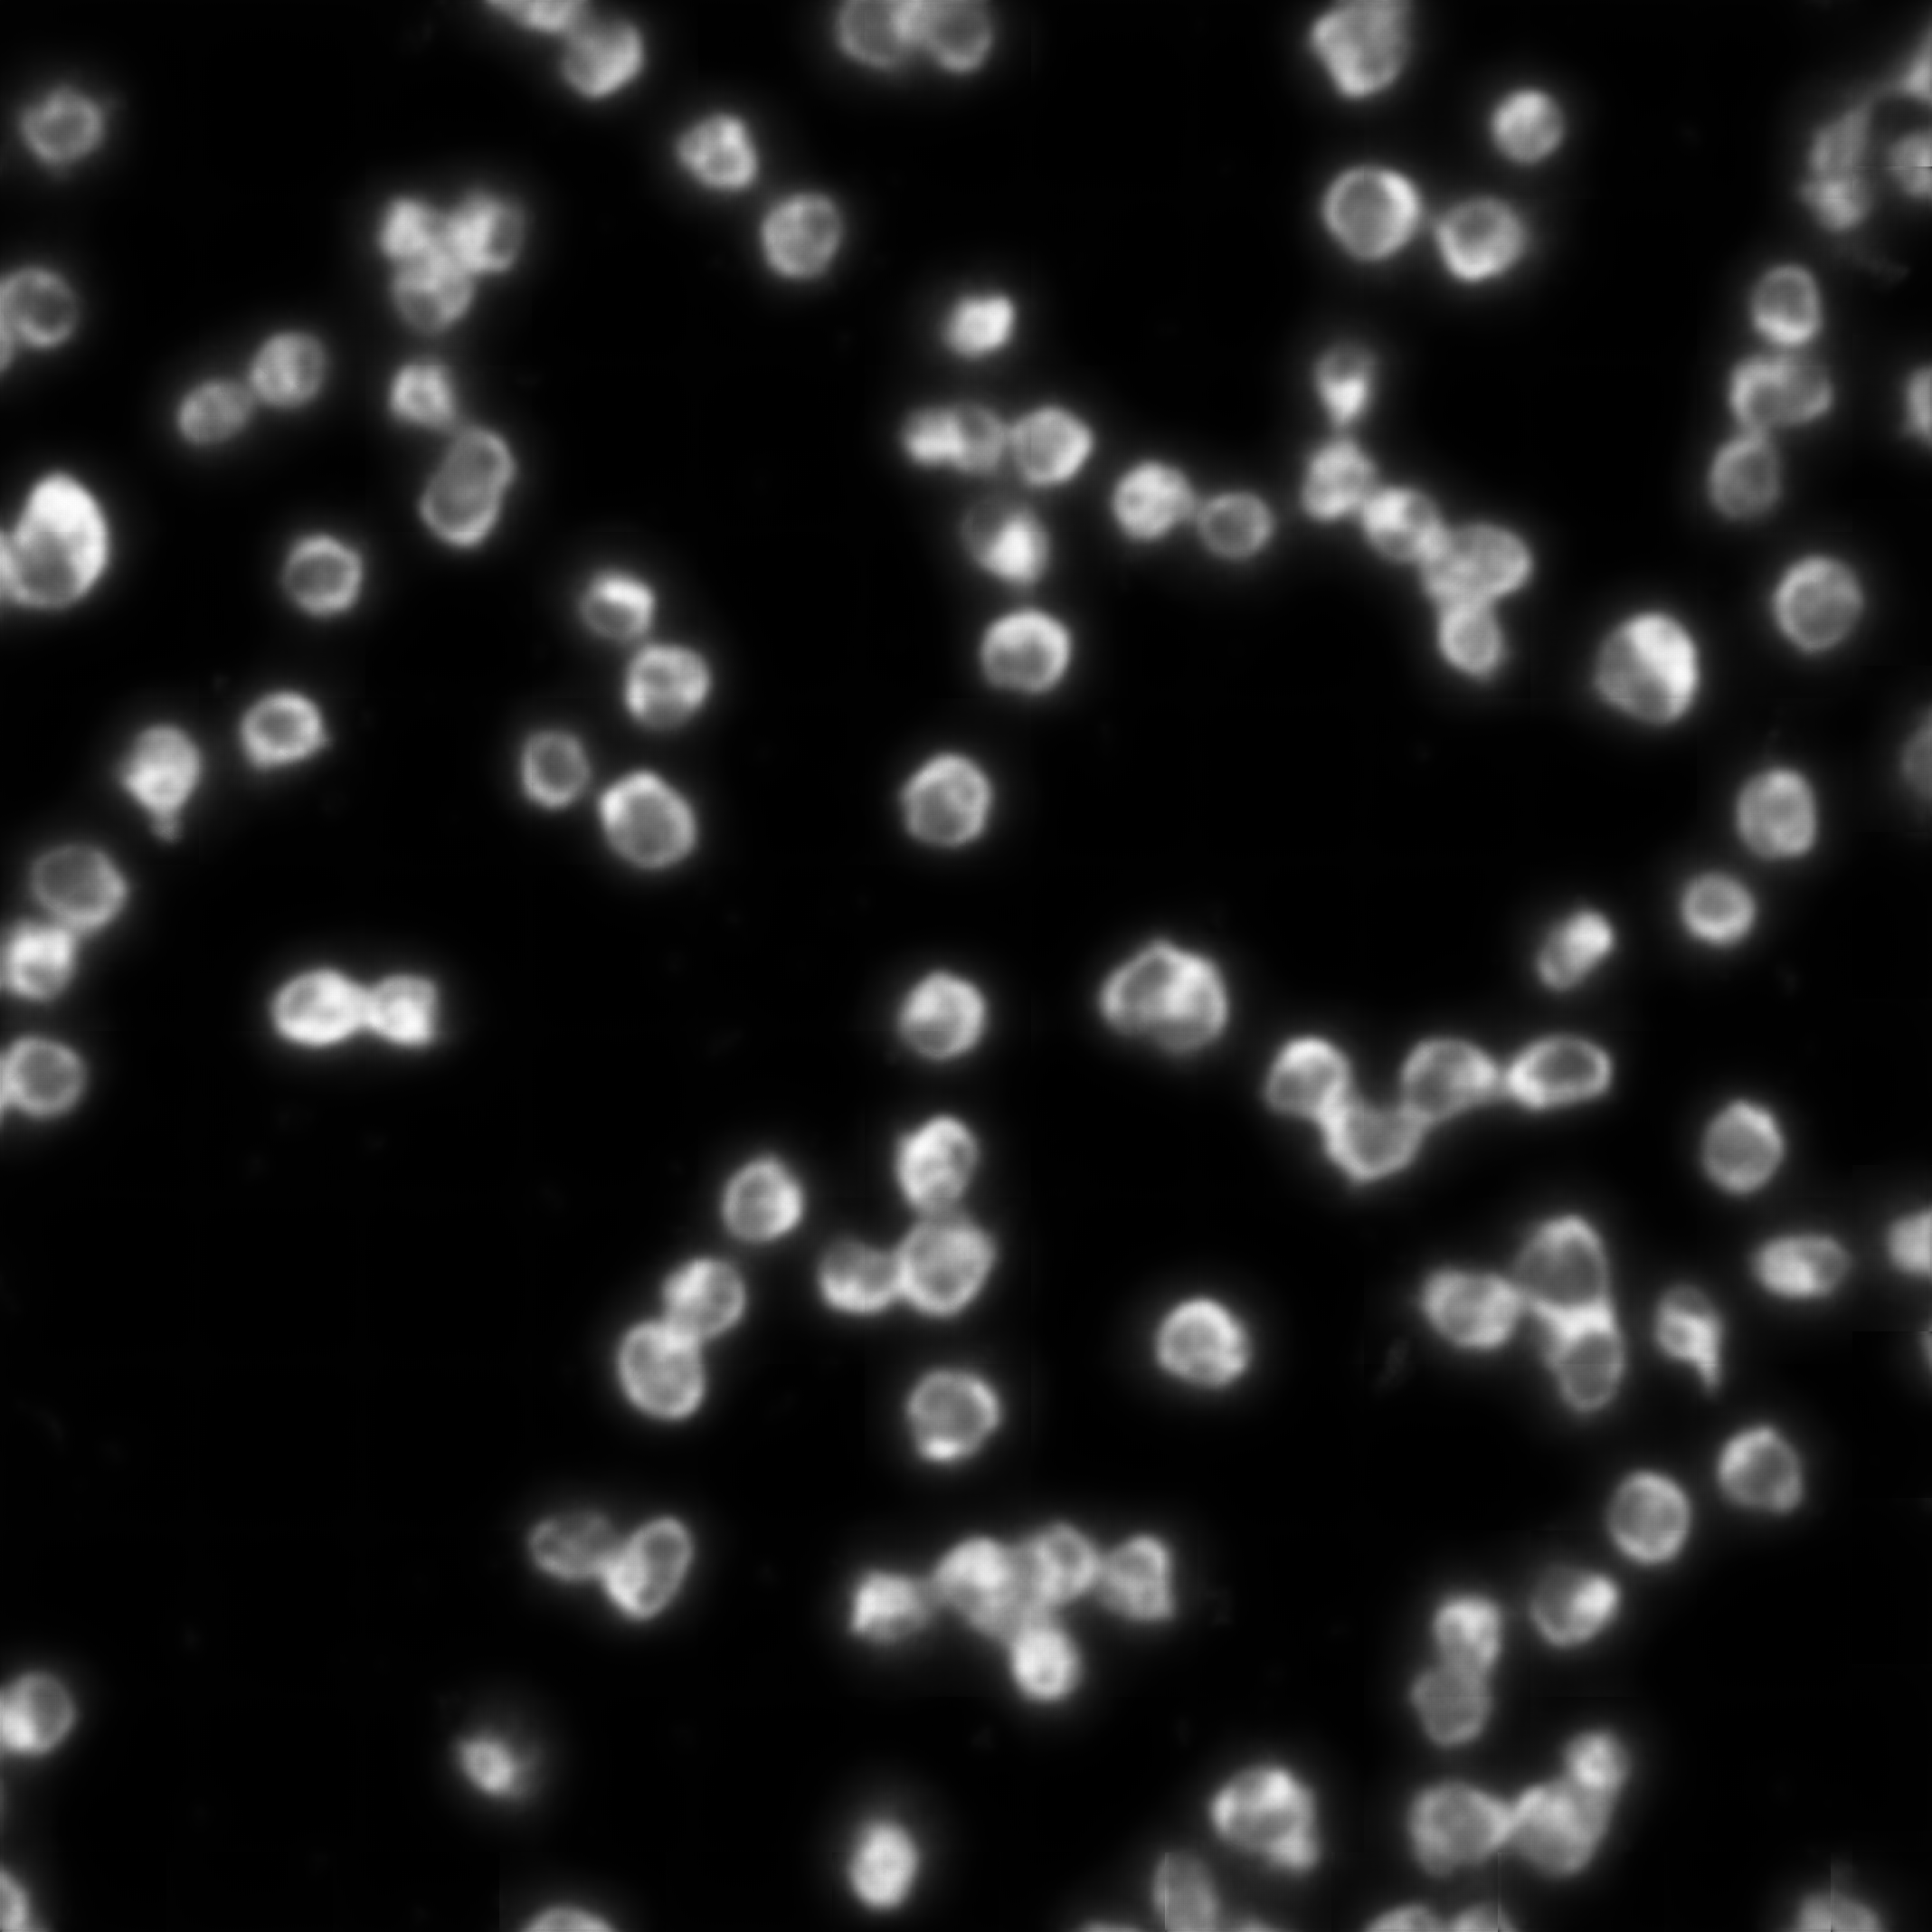
\includegraphics{bilder/ER/segmentation/pp_1.png} & 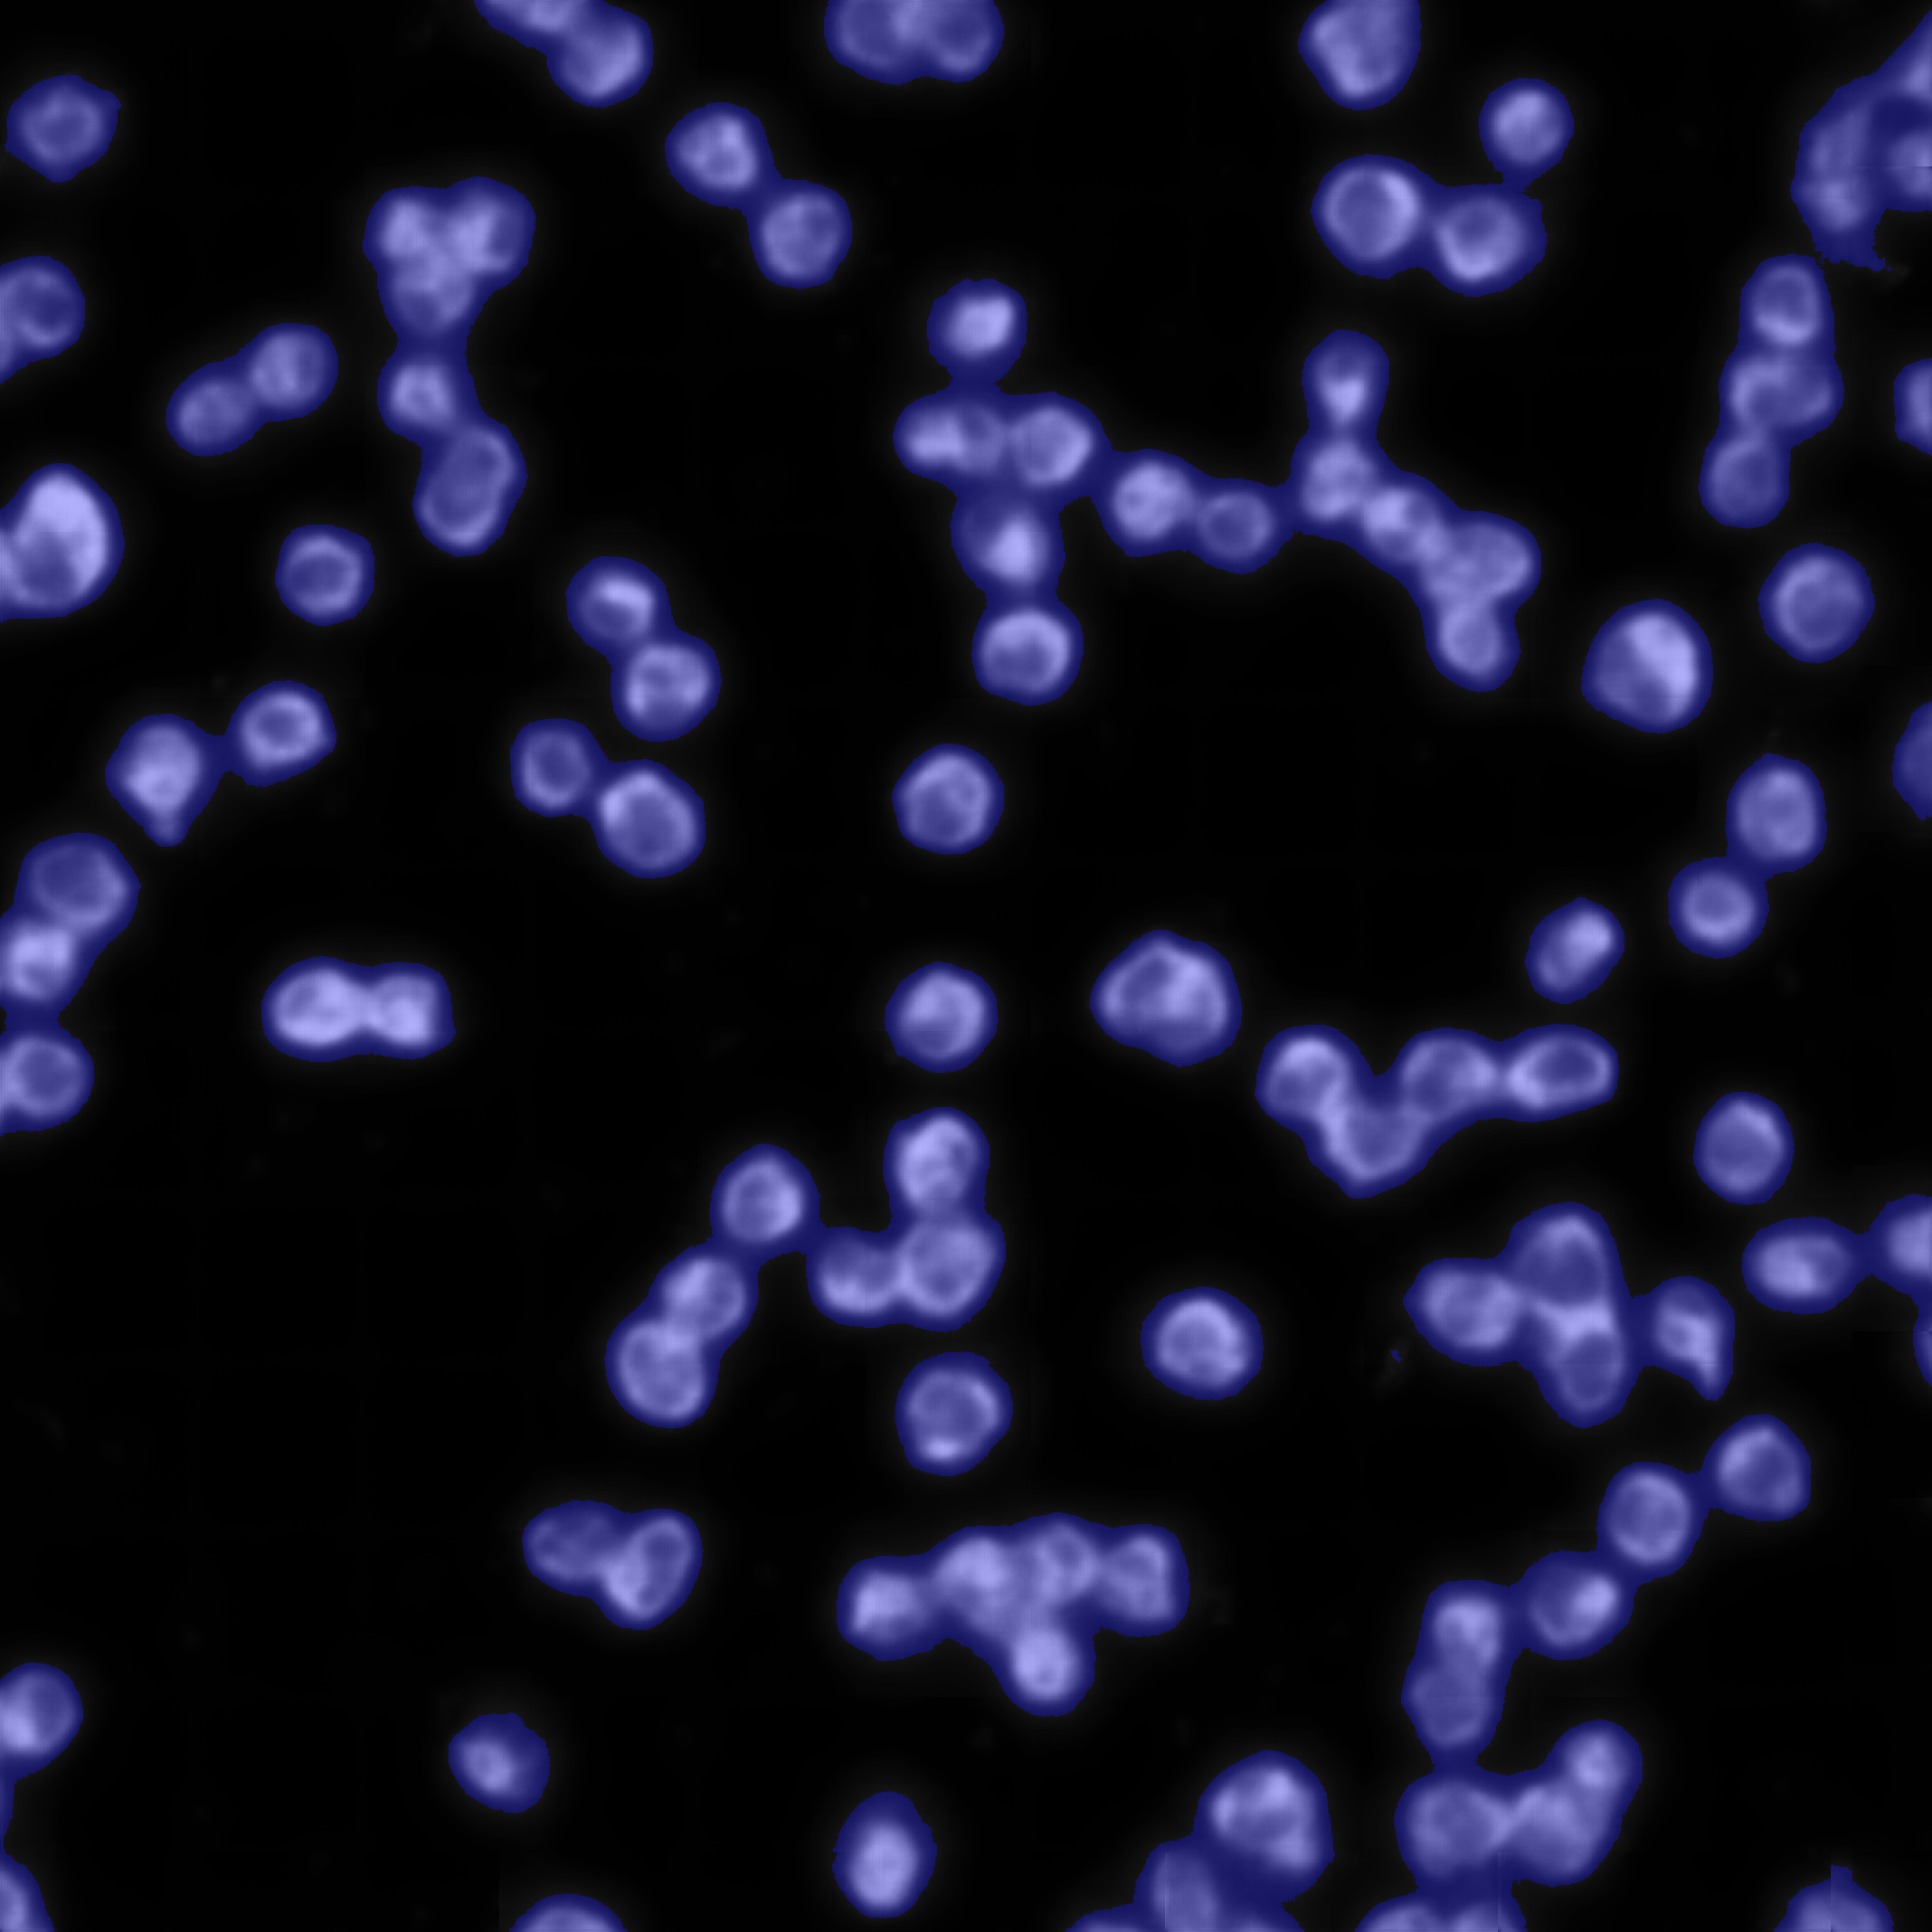
\includegraphics{bilder/ER/segmentation/pp_2.png} &
            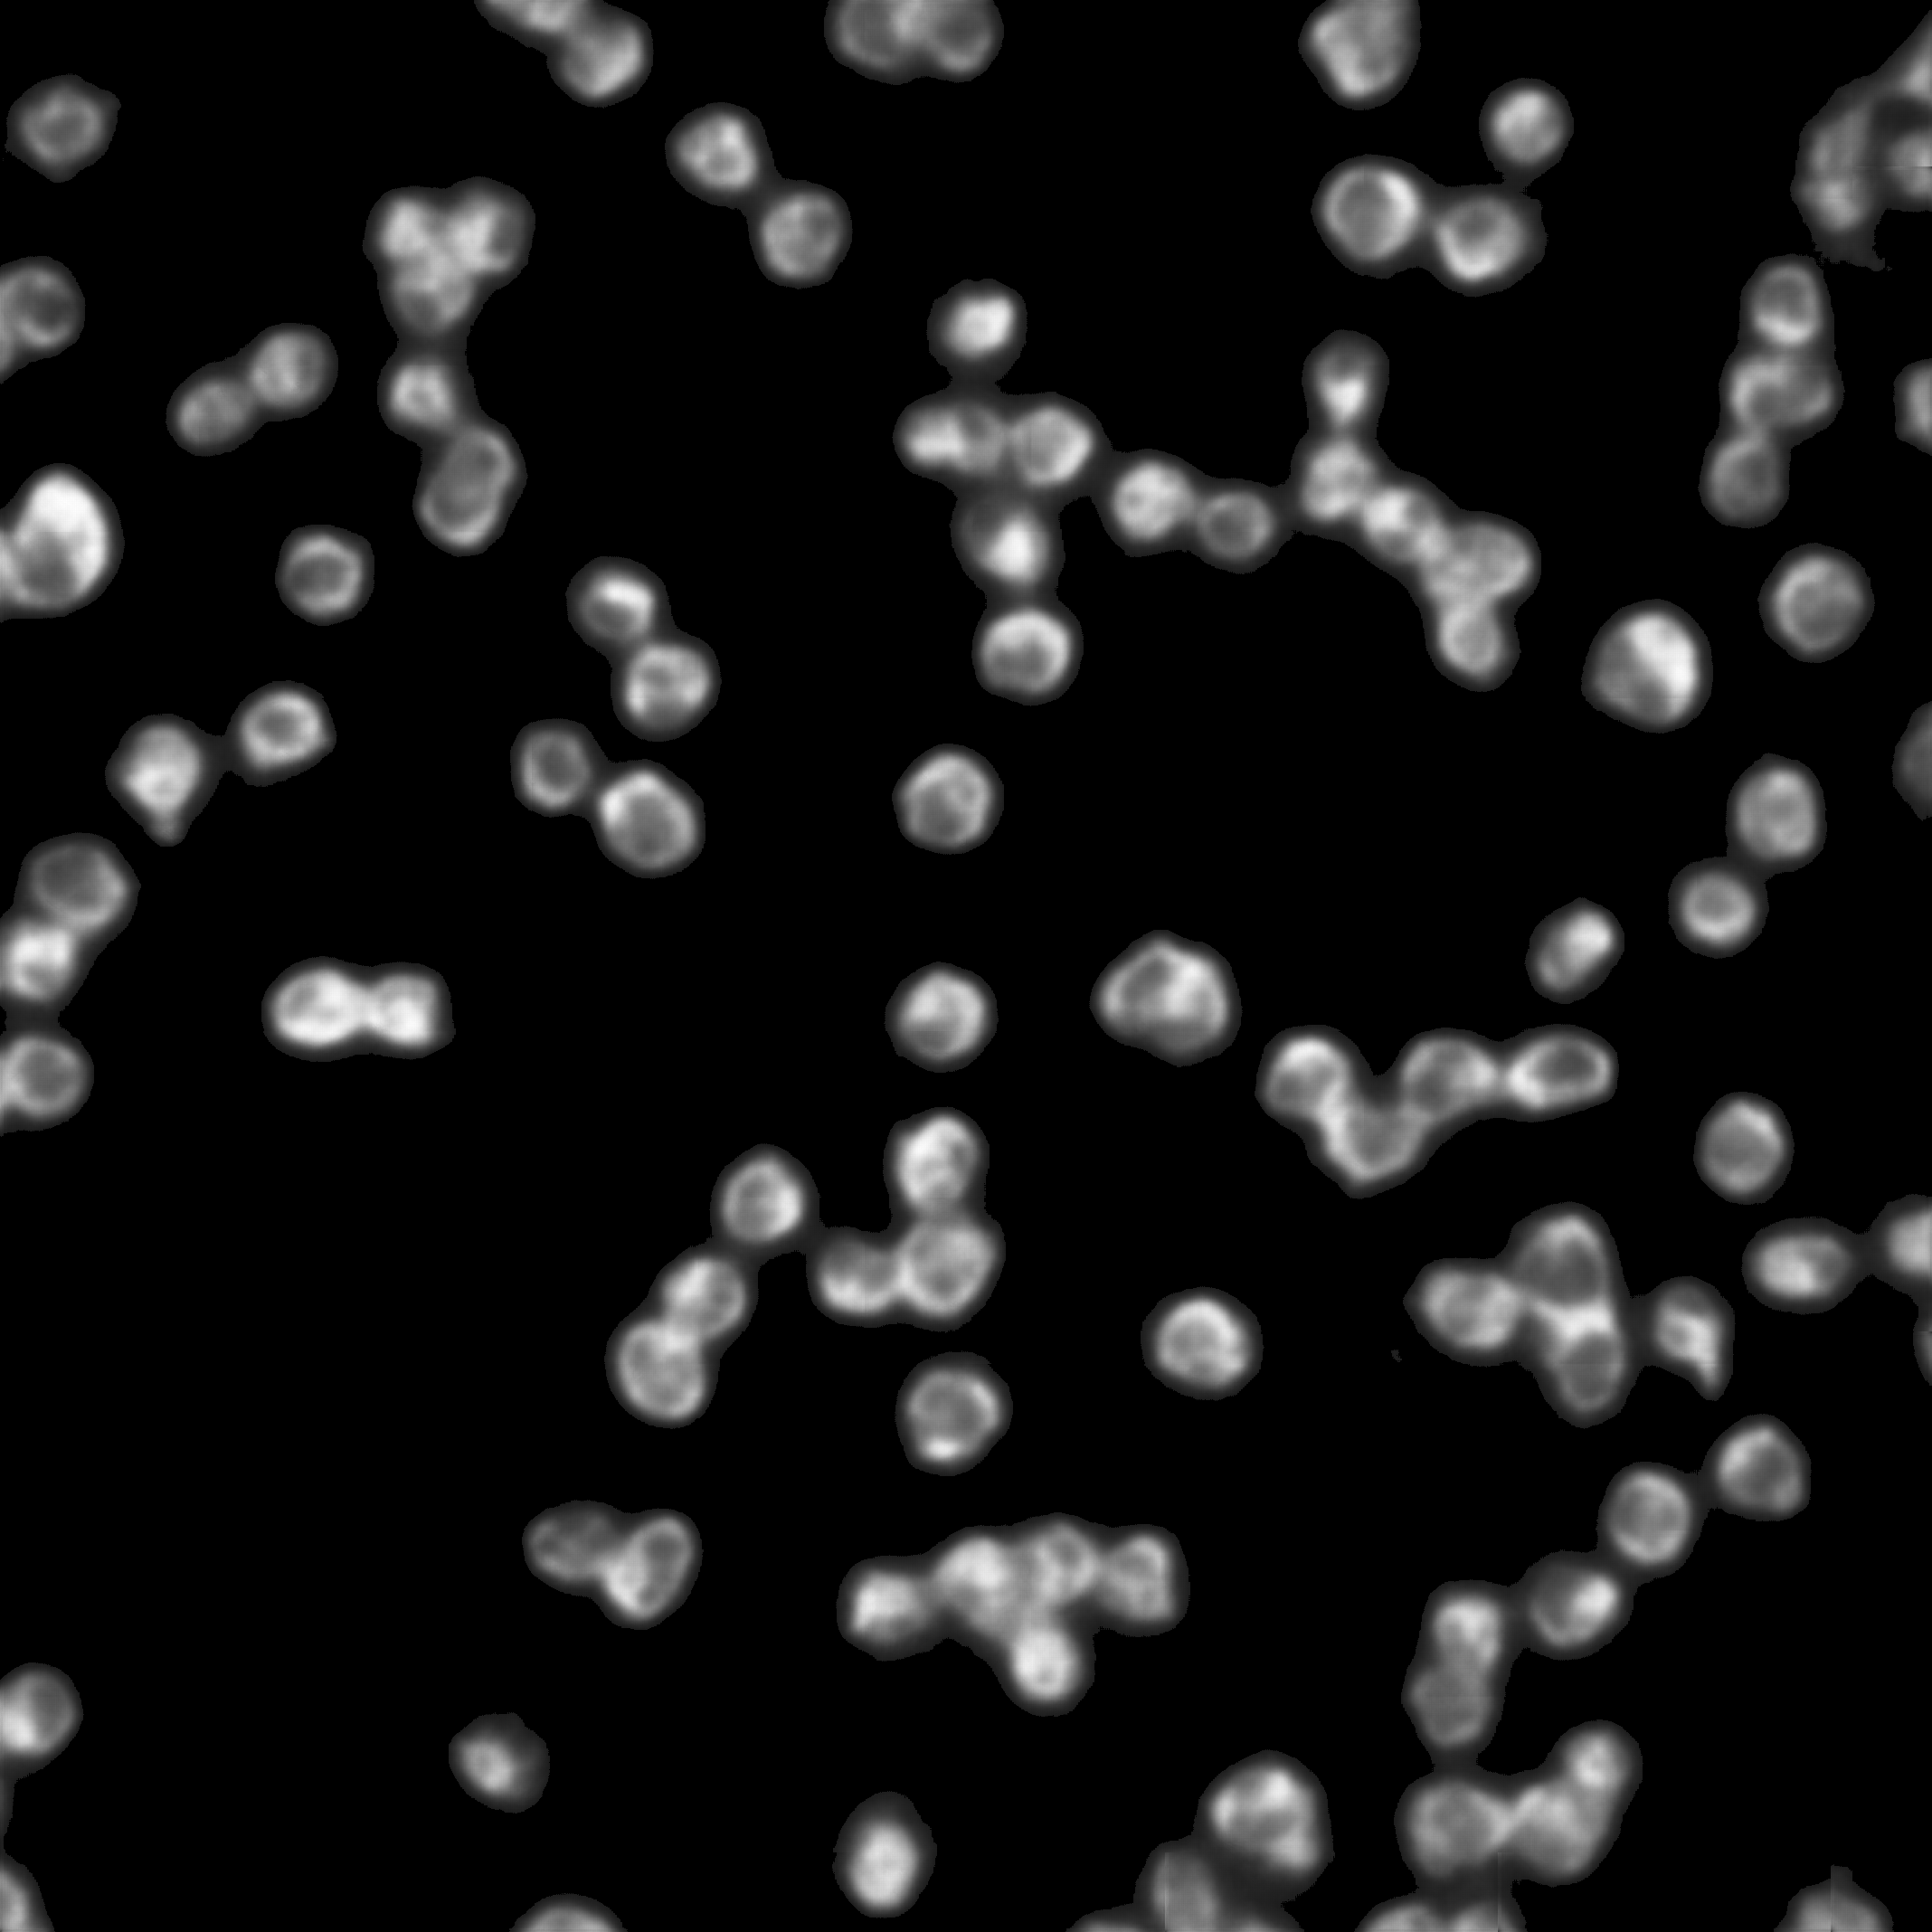
\includegraphics{bilder/ER/segmentation/pp_3.png} &
            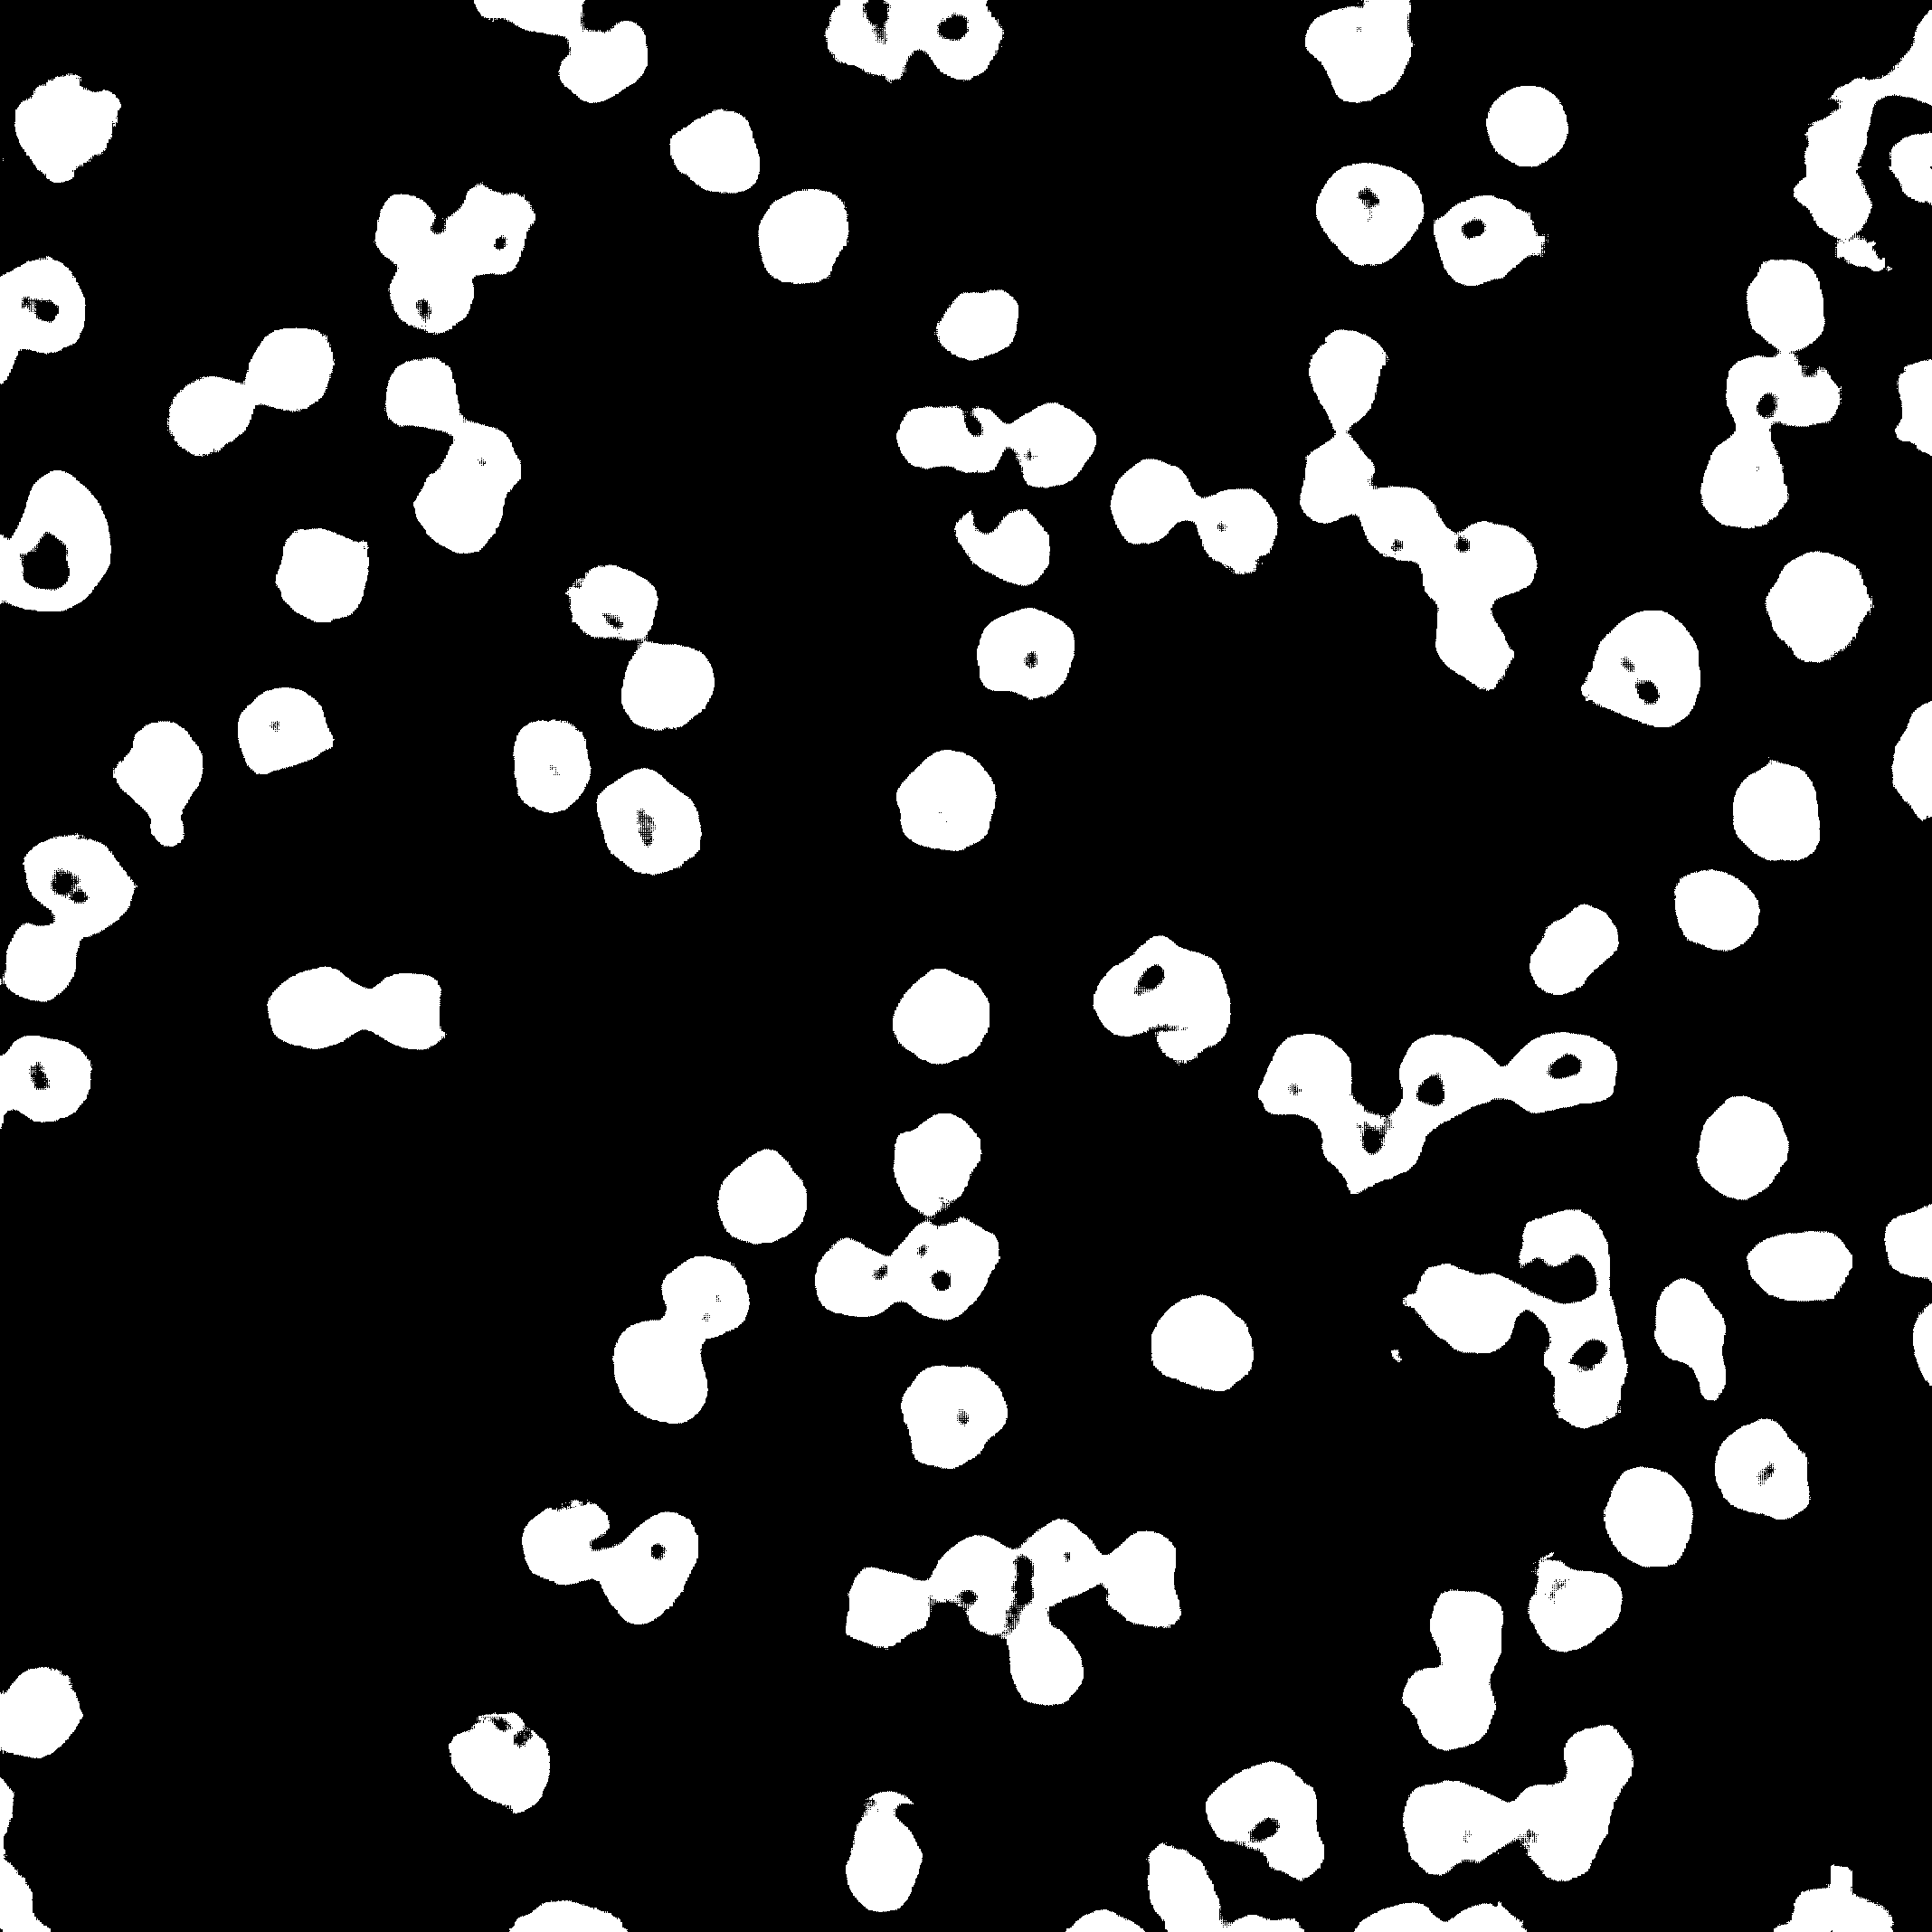
\includegraphics{bilder/ER/segmentation/pp_4.png} &
            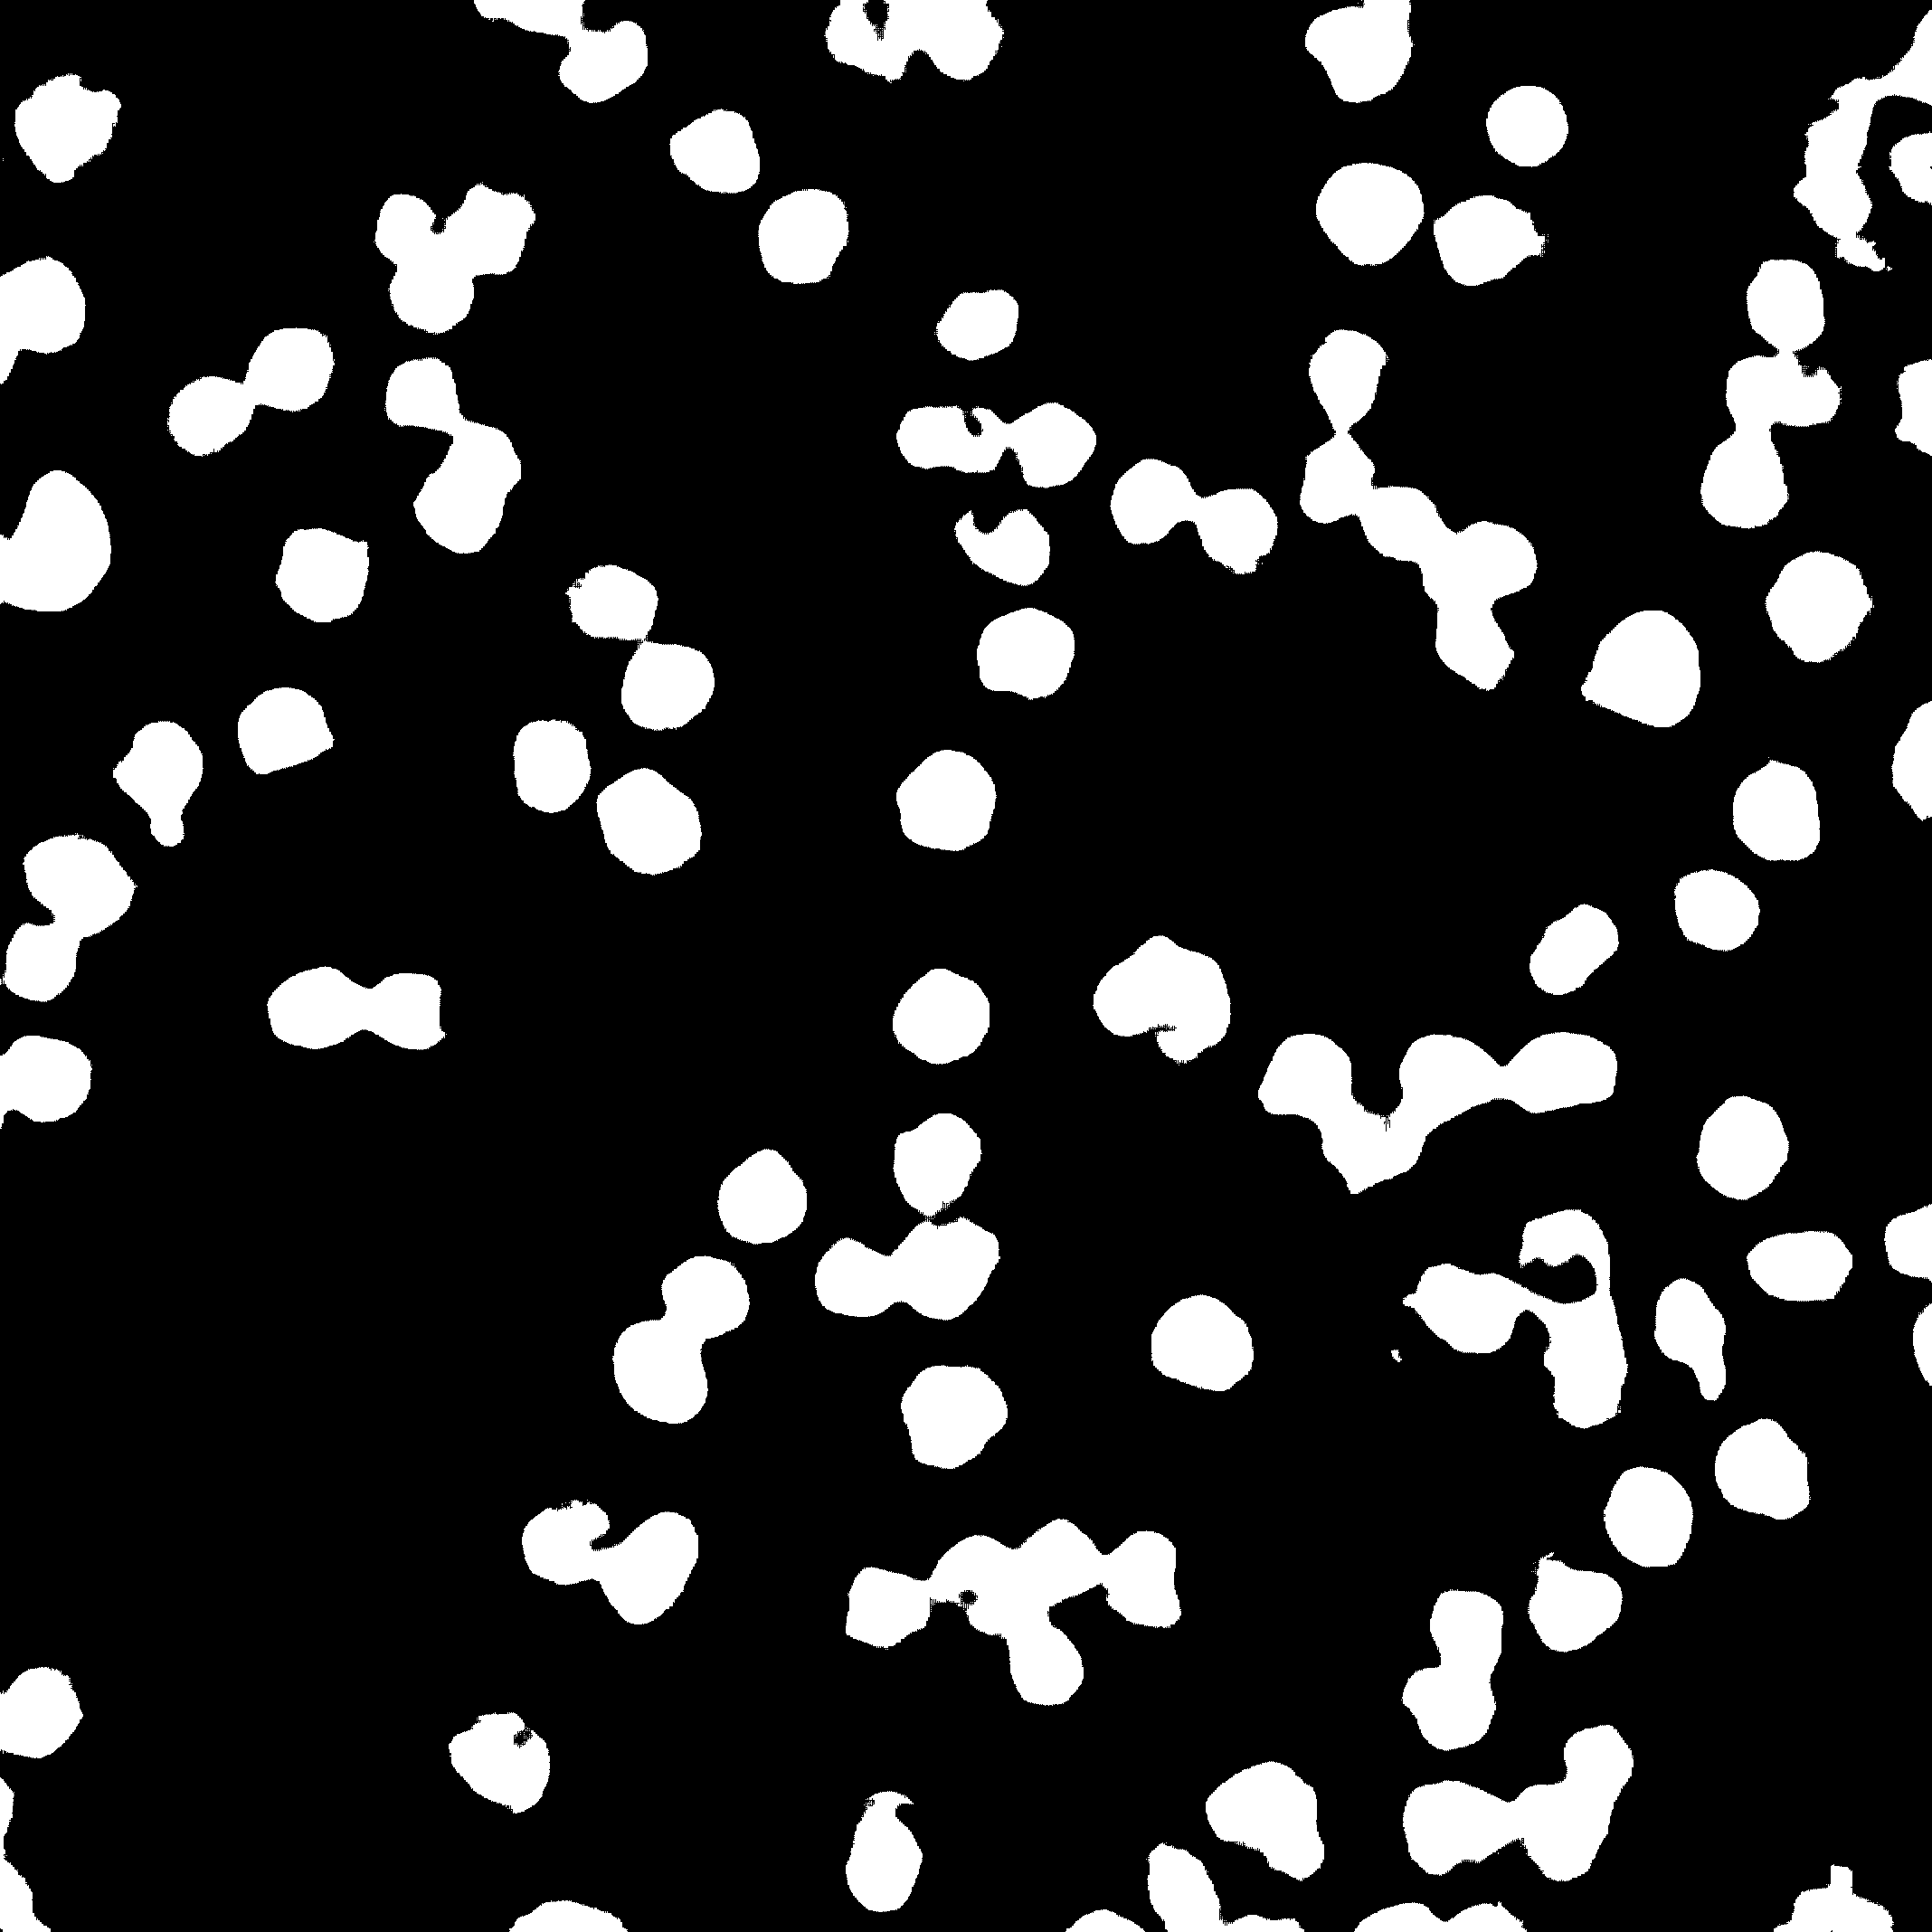
\includegraphics{bilder/ER/segmentation/pp_5.png} &
            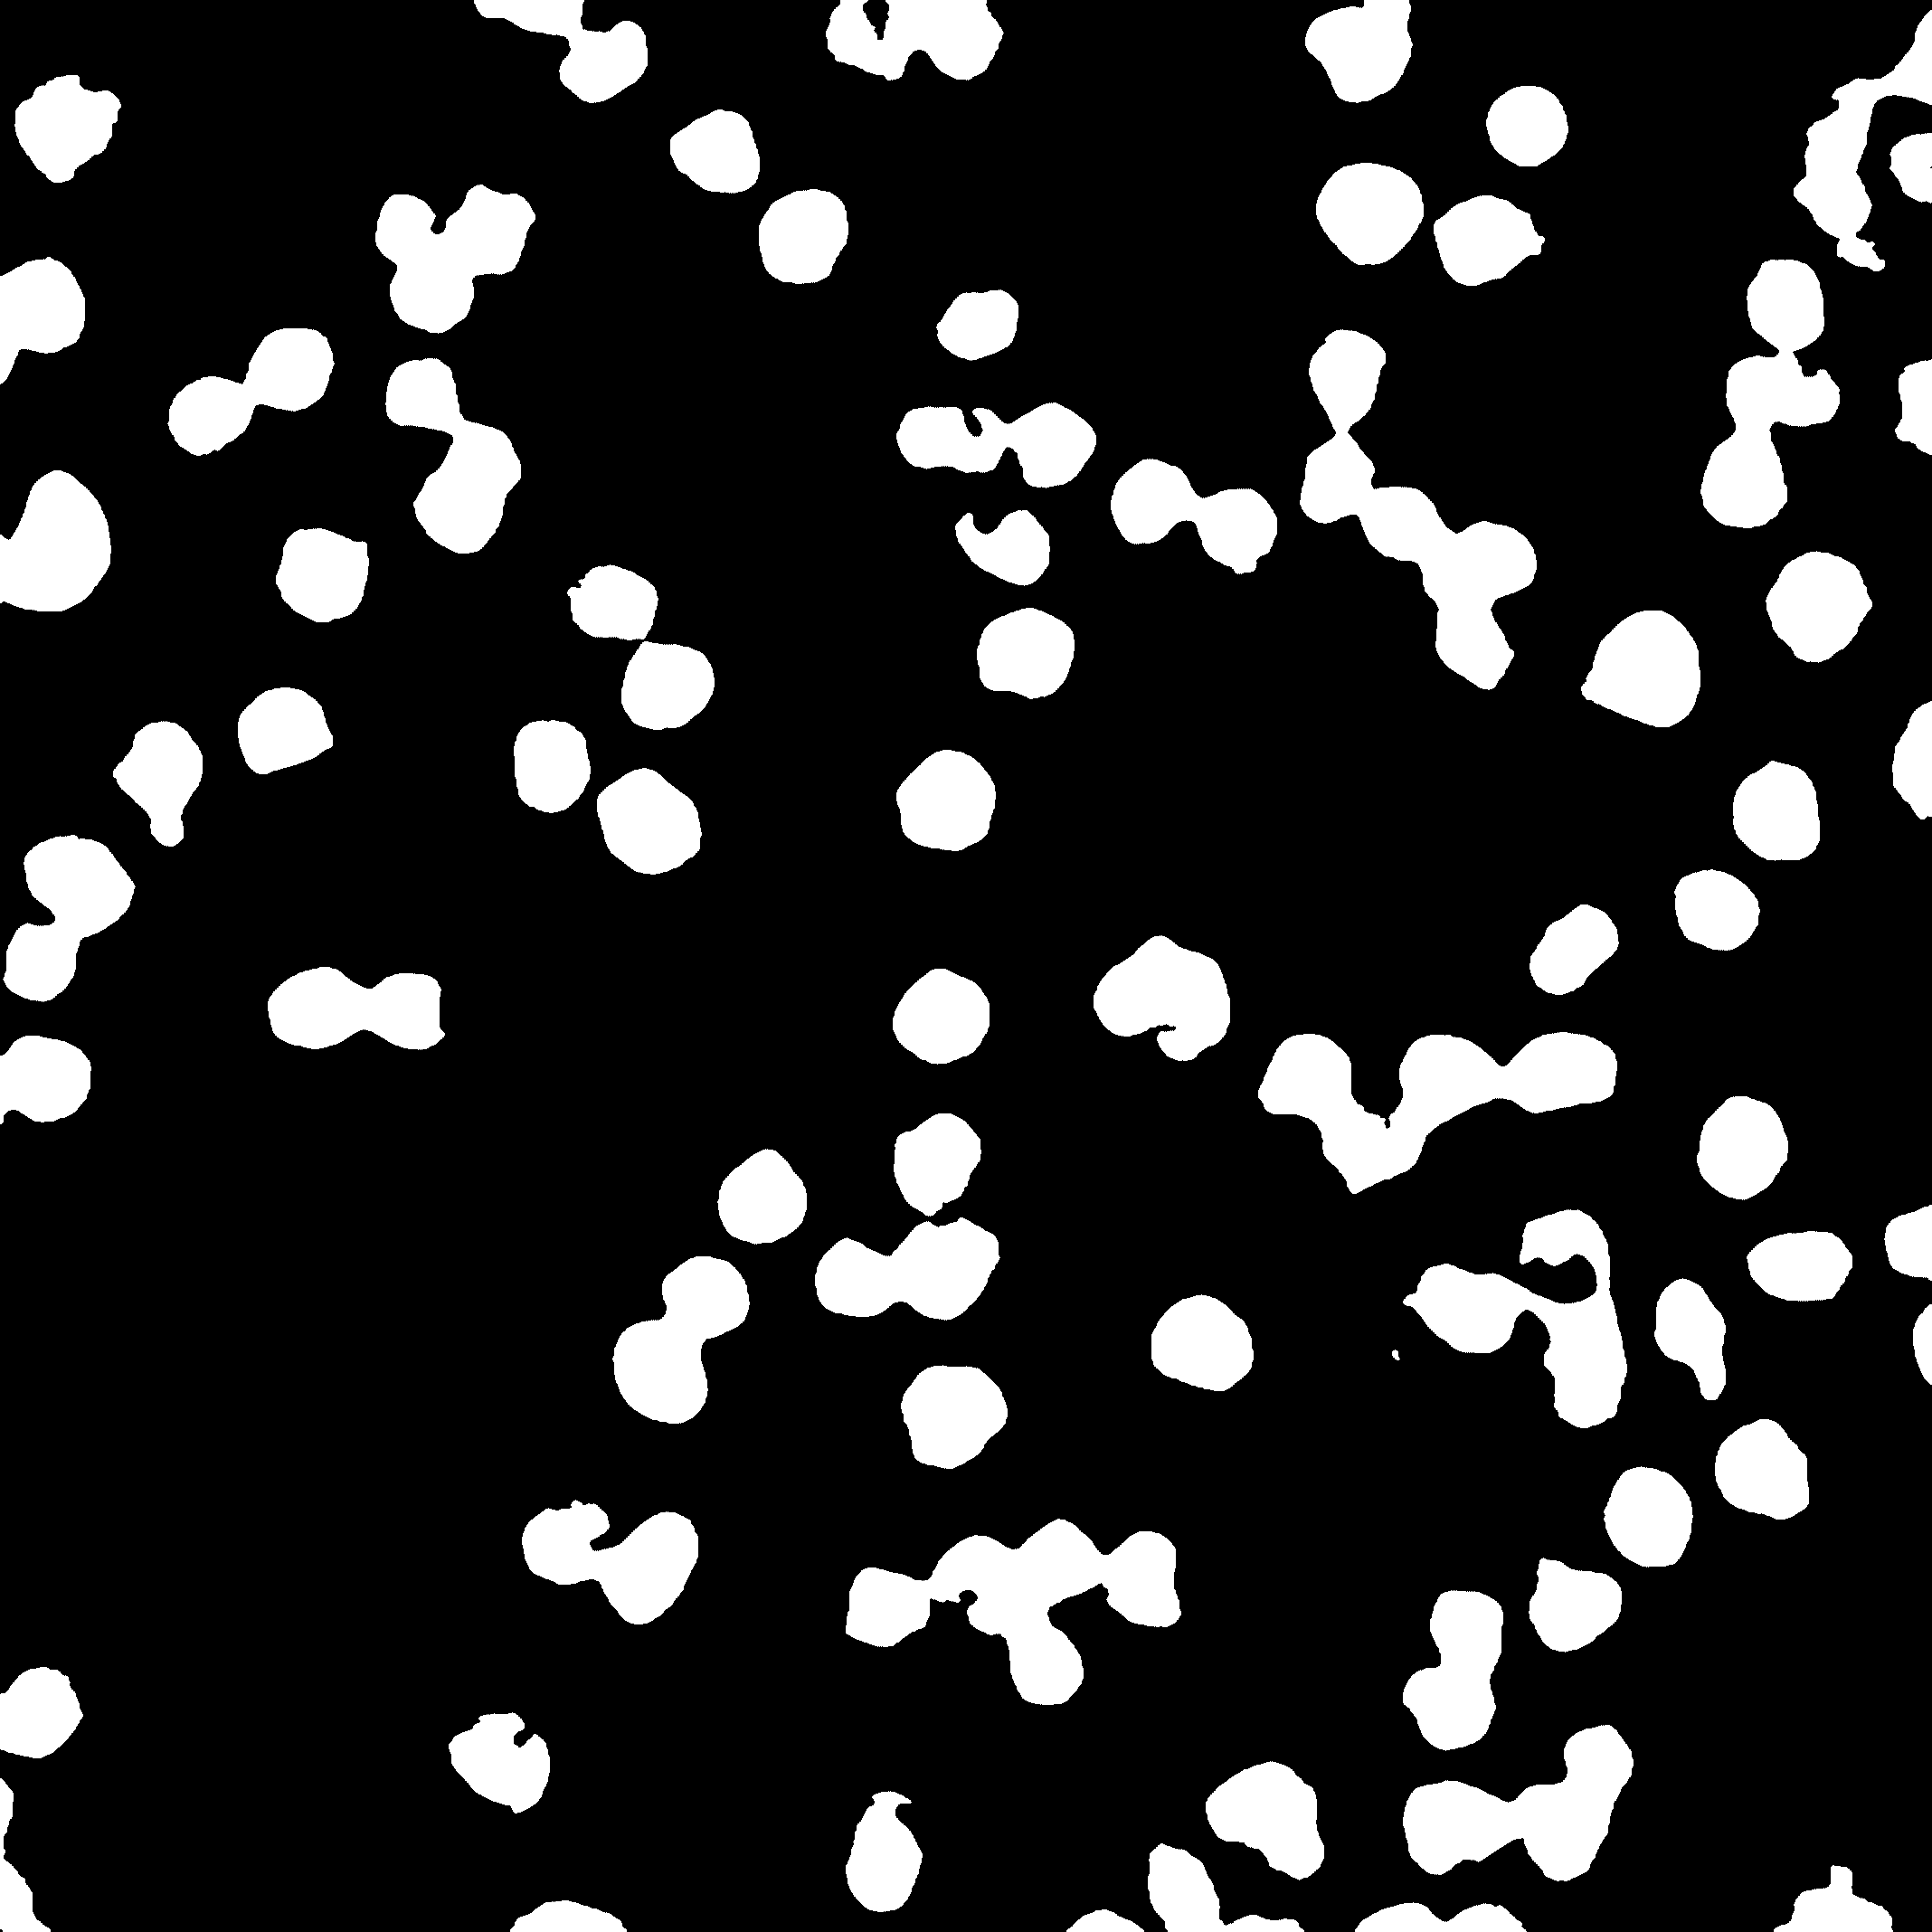
\includegraphics{bilder/ER/segmentation/pp_6.png} &
            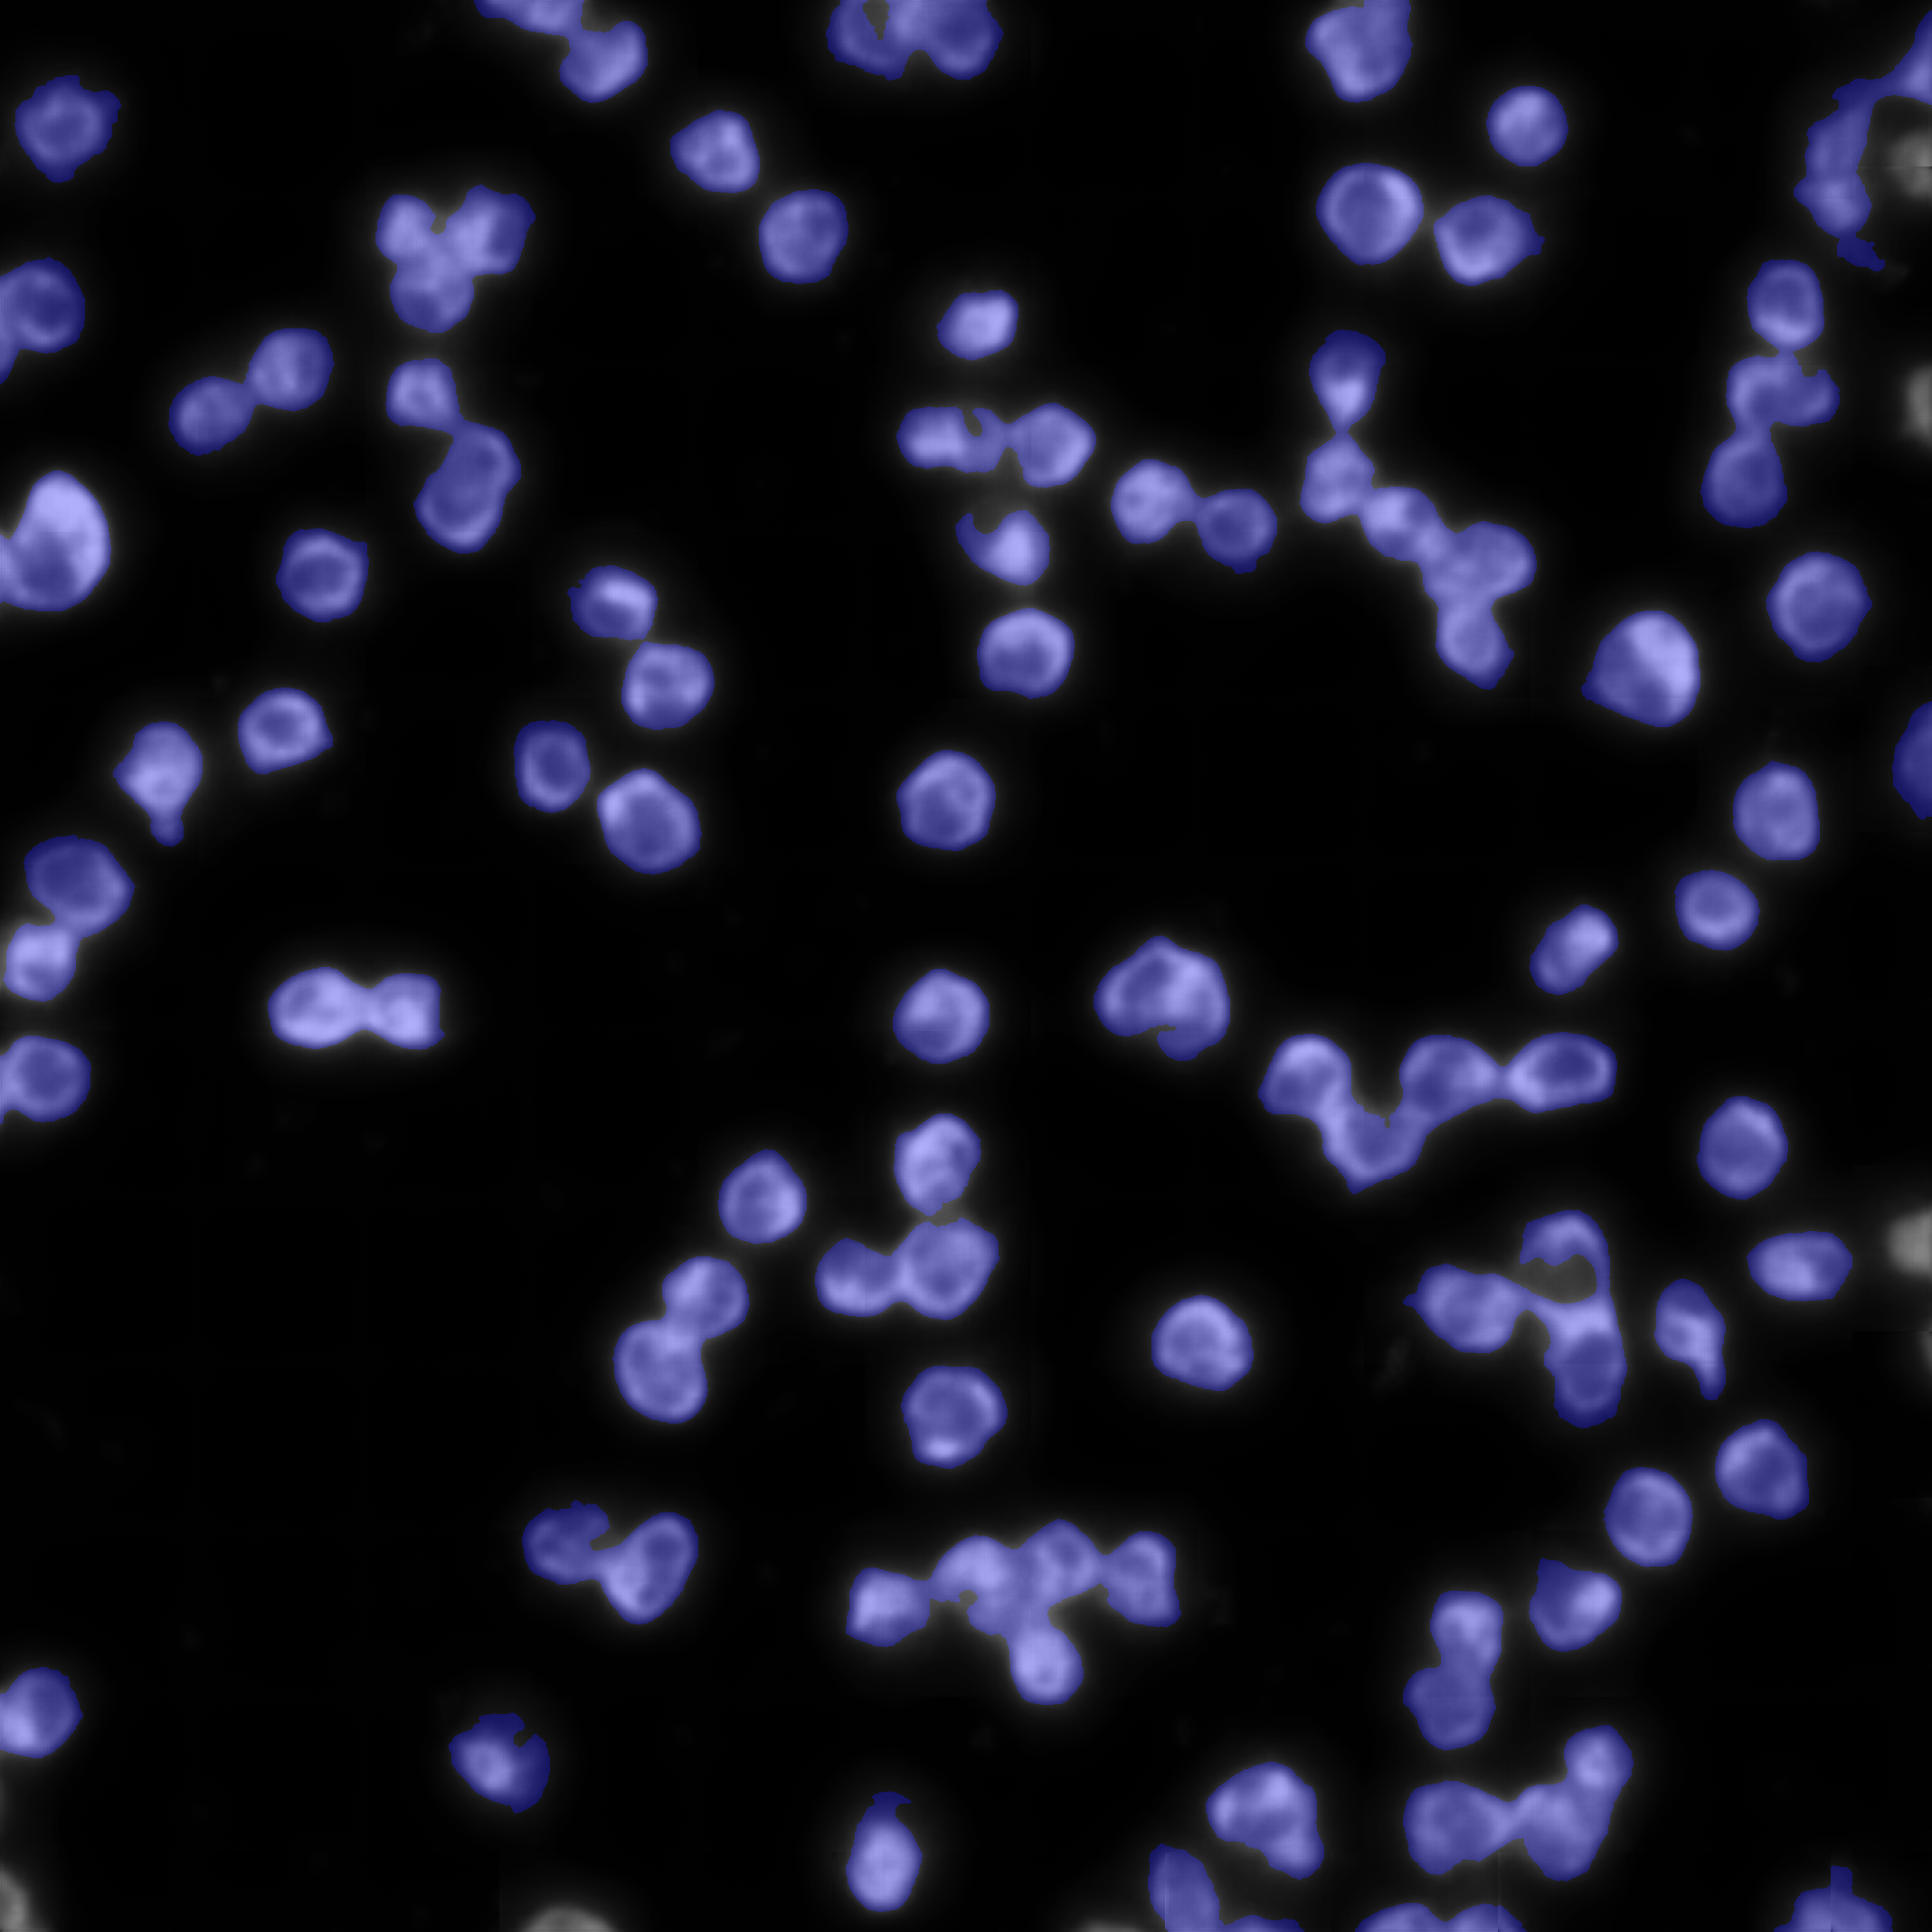
\includegraphics{bilder/ER/segmentation/pp_7.png} 
        \end{tabularx}
    \caption{ER prediction}
    \label{fig:er-prediction}
\end{figure}


\subsection{Golgi}
